%%%%%%%%%%%%%%%%%%%%%%%%%%%%%%%%%%%%%%%%%%%%%%%%%%%%%%%%%%%%%%%%%%%%%%
% Template for a UBC-compliant dissertation
% At the minimum, you will need to change the information found
% after the "Document meta-data"
%
%!TEX TS-program = pdflatex
%!TEX encoding = UTF-8 Unicode

%% The ubcdiss class provides several options:
%%   gpscopy (aka fogscopy)
%%       set parameters to exactly how GPS specifies
%%         * single-sided
%%         * page-numbering starts from title page
%%         * the lists of figures and tables have each entry prefixed
%%           with 'Figure' or 'Table'
%%       This can be tested by `\ifgpscopy ... \else ... \fi'
%%   10pt, 11pt, 12pt
%%       set default font size
%%   oneside, twoside
%%       whether to format for single-sided or double-sided printing
%%   balanced
%%       when double-sided, ensure page content is centred
%%       rather than slightly offset (the default)
%%   singlespacing, onehalfspacing, doublespacing
%%       set default inter-line text spacing; the ubcdiss class
%%       provides \textspacing to revert to this configured spacing
%%   draft
%%       disable more intensive processing, such as including
%%       graphics, etc.
%%

% For submission to GPS
\documentclass[gpscopy,onehalfspacing,11pt]{ubcdiss}

% For your own copies (looks nicer)
% \documentclass[balanced,twoside,11pt]{ubcdiss}

%%%%%%%%%%%%%%%%%%%%%%%%%%%%%%%%%%%%%%%%%%%%%%%%%%%%%%%%%%%%%%%%%%%%%%
%%%%%%%%%%%%%%%%%%%%%%%%%%%%%%%%%%%%%%%%%%%%%%%%%%%%%%%%%%%%%%%%%%%%%%
%%
%% FONTS:
%% 
%% The defaults below configures Times Roman for the serif font,
%% Helvetica for the sans serif font, and Courier for the
%% typewriter-style font.  Configuring fonts can be time
%% consuming; we recommend skipping to END FONTS!
%% 
%% If you're feeling brave, have lots of time, and wish to use one
%% your platform's native fonts, see the commented out bits below for
%% XeTeX/XeLaTeX.  This is not for the faint at heart. 
%% (And shouldn't you be writing? :-)
%%

%% NFSS font specification (New Font Selection Scheme)
\usepackage{times,mathptmx,courier}
\usepackage[scaled=.92]{helvet}

%% Math or theory people may want to include the handy AMS macros
%\usepackage{amssymb}
%\usepackage{amsmath}
%\usepackage{amsfonts}

%% The pifont package provides access to the elements in the dingbat font.   
%% Use \ding{##} for a particular dingbat (see p7 of psnfss2e.pdf)
%%   Useful:
%%     51,52 different forms of a checkmark
%%     54,55,56 different forms of a cross (saltyre)
%%     172-181 are 1-10 in open circle (serif)
%%     182-191 are 1-10 black circle (serif)
%%     192-201 are 1-10 in open circle (sans serif)
%%     202-211 are 1-10 in black circle (sans serif)
%% \begin{dinglist}{##}\item... or dingautolist (which auto-increments)
%% to create a bullet list with the provided character.
\usepackage{pifont}

%%%%%%%%%%%%%%%%%%%%%%%%%%%%%%%%%%%%%%%%%%%%%%%%%%%%%%%%%%%%%%%%%%%%%%
%% Configure fonts for XeTeX / XeLaTeX using the fontspec package.
%% Be sure to check out the fontspec documentation.
%\usepackage{fontspec,xltxtra,xunicode}	% required
%\defaultfontfeatures{Mapping=tex-text}	% recommended
%% Minion Pro and Myriad Pro are shipped with some versions of
%% Adobe Reader.  Adobe representatives have commented that these
%% fonts can be used outside of Adobe Reader.
%\setromanfont[Numbers=OldStyle]{Minion Pro}
%\setsansfont[Numbers=OldStyle,Scale=MatchLowercase]{Myriad Pro}
%\setmonofont[Scale=MatchLowercase]{Andale Mono}

%% Other alternatives:
%\setromanfont[Mapping=tex-text]{Adobe Caslon}
%\setsansfont[Scale=MatchLowercase]{Gill Sans}
%\setsansfont[Scale=MatchLowercase,Mapping=tex-text]{Futura}
%\setmonofont[Scale=MatchLowercase]{Andale Mono}
%\newfontfamily{\SYM}[Scale=0.9]{Zapf Dingbats}
%% END FONTS
%%%%%%%%%%%%%%%%%%%%%%%%%%%%%%%%%%%%%%%%%%%%%%%%%%%%%%%%%%%%%%%%%%%%%%
%%%%%%%%%%%%%%%%%%%%%%%%%%%%%%%%%%%%%%%%%%%%%%%%%%%%%%%%%%%%%%%%%%%%%%



%%%%%%%%%%%%%%%%%%%%%%%%%%%%%%%%%%%%%%%%%%%%%%%%%%%%%%%%%%%%%%%%%%%%%%
%%%%%%%%%%%%%%%%%%%%%%%%%%%%%%%%%%%%%%%%%%%%%%%%%%%%%%%%%%%%%%%%%%%%%%
%%
%% Recommended packages
%%
\usepackage{checkend}	% better error messages on left-open environments
\usepackage{graphicx}	% for incorporating external images

%% booktabs: provides some special commands for typesetting tables as used
%% in excellent journals.  Ignore the examples in the Lamport book!
\usepackage{booktabs}

%% listings: useful support for including source code listings, with
%% optional special keyword formatting.  The \lstset{} causes
%% the text to be typeset in a smaller sans serif font, with
%% proportional spacing.
\usepackage{listings}
\lstset{basicstyle=\sffamily\scriptsize,showstringspaces=false,fontadjust}

%% The acronym package provides support for defining acronyms, providing
%% their expansion when first used, and building glossaries.  See the
%% example in glossary.tex and the example usage throughout the example
%% document.
%% NOTE: to use \MakeTextLowercase in the \acsfont command below,
%%   we *must* use the `nohyperlinks' option -- it causes errors with
%%   hyperref otherwise.  See Section 5.2 in the ``LaTeX 2e for Class
%%   and Package Writers Guide'' (clsguide.pdf) for details.
\usepackage[printonlyused,nohyperlinks]{acronym}
%% The ubcdiss.cls loads the `textcase' package which provides commands
%% for upper-casing and lower-casing text.  The following causes
%% the acronym package to typeset acronyms in small-caps
%% as recommended by Bringhurst.
\renewcommand{\acsfont}[1]{{\scshape \MakeTextLowercase{#1}}}

%% color: add support for expressing colour models.  Grey can be used
%% to great effect to emphasize other parts of a graphic or text.
%% For an excellent set of examples, see Tufte's "Visual Display of
%% Quantitative Information" or "Envisioning Information".
\usepackage{color}
\definecolor{greytext}{gray}{0.5}

%% comment: provides a new {comment} environment: all text inside the
%% environment is ignored.
%%   \begin{comment} ignored text ... \end{comment}
\usepackage{comment}

%% The natbib package provides more sophisticated citing commands
%% such as \citeauthor{} to provide the author names of a work,
%% \citet{} to produce an author-and-reference citation,
%% \citep{} to produce a parenthetical citation.
%% We use \citeeg{} to provide examples
\usepackage[numbers,sort&compress]{natbib}
\newcommand{\citeeg}[1]{\citep[e.g.,][]{#1}}

%% The titlesec package provides commands to vary how chapter and
%% section titles are typeset.  The following uses more compact
%% spacings above and below the title.  The titleformat that follow
%% ensure chapter/section titles are set in singlespace.
\usepackage[compact]{titlesec}
\titleformat*{\section}{\singlespacing\raggedright\bfseries\Large}
\titleformat*{\subsection}{\singlespacing\raggedright\bfseries\large}
\titleformat*{\subsubsection}{\singlespacing\raggedright\bfseries}
\titleformat*{\paragraph}{\singlespacing\raggedright\itshape}

%% The caption package provides support for varying how table and
%% figure captions are typeset.
\usepackage[format=hang,indention=-1cm,labelfont={bf},margin=1em]{caption}

%% url: for typesetting URLs and smart(er) hyphenation.
%% \url{http://...} 
\usepackage{url}
\urlstyle{sf}	% typeset urls in sans-serif

%% math
\usepackage{amsthm}

%%%%%%%%%%%%%%%%%%%%%%%%%%%%%%%%%%%%%%%%%%%%%%%%%%%%%%%%%%%%%%%%%%%%%%
%%%%%%%%%%%%%%%%%%%%%%%%%%%%%%%%%%%%%%%%%%%%%%%%%%%%%%%%%%%%%%%%%%%%%%
%%
%% Possibly useful packages: you may need to explicitly install
%% these from CTAN if they aren't part of your distribution;
%% teTeX seems to ship with a smaller base than MikTeX and MacTeX.
%%
%\usepackage{pdfpages}	% insert pages from other PDF files
%\usepackage{longtable}	% provide tables spanning multiple pages
%\usepackage{chngpage}	% support changing the page widths on demand
%\usepackage{tabularx}	% an enhanced tabular environment

%% enumitem: support pausing and resuming enumerate environments.
%\usepackage{enumitem}

%% rotating: provides two environments, sidewaystable and sidewaysfigure,
%% for typesetting tables and figures in landscape mode.  
%\usepackage{rotating}

%% subfig: provides for including subfigures within a figure,
%% and includes being able to separately reference the subfigures.
%\usepackage{subfig}

%% ragged2e: provides several new new commands \Centering, \RaggedLeft,
%% \RaggedRight and \justifying and new environments Center, FlushLeft,
%% FlushRight and justify, which set ragged text and are easily
%% configurable to allow hyphenation.
%\usepackage{ragged2e}

%% The ulem package provides a \sout{} for striking out text and
%% \xout for crossing out text.  The normalem and normalbf are
%% necessary as the package messes with the emphasis and bold fonts
%% otherwise.
%\usepackage[normalem,normalbf]{ulem}    % for \sout

%%%%%%%%%%%%%%%%%%%%%%%%%%%%%%%%%%%%%%%%%%%%%%%%%%%%%%%%%%%%%%%%%%%%%%
%% HYPERREF:
%% The hyperref package provides for embedding hyperlinks into your
%% document.  By default the table of contents, references, citations,
%% and footnotes are hyperlinked.
%%
%% Hyperref provides a very handy command for doing cross-references:
%% \autoref{}.  This is similar to \ref{} and \pageref{} except that
%% it automagically puts in the *type* of reference.  For example,
%% referencing a figure's label will put the text `Figure 3.4'.
%% And the text will be hyperlinked to the appropriate place in the
%% document.
%%
%% Generally hyperref should appear after most other packages

%% The `pagebackref' causes the references in the bibliography to have
%% back-references to the citing page; `backref' puts the citing section
%% number.  See further below for other examples of using hyperref.
%% 2009/12/09: now use `linktocpage' (Jacek Kisynski): GPS now prefers
%%   that the ToC, LoF, LoT place the hyperlink on the page number,
%%   rather than the entry text.
\ifgpscopy
  % GPS requires that weblinks should be dark blue, which looks a bit
  % odd in printed form.
  % https://www.grad.ubc.ca/current-students/dissertation-thesis-preparation/fonts-print
  \usepackage[bookmarks,bookmarksnumbered,%
     pagebackref,linktocpage,%
     colorlinks=true,%
     linkcolor=black,%
     urlcolor=blue,%
     citecolor=black%
     ]{hyperref}
\else
  %% The following puts hyperlinks in very faint grey boxes (in pdf only).
  \usepackage[bookmarks,bookmarksnumbered,%
    pagebackref,linktocpage,%
    allbordercolors={0.8 0.8 0.8},%
    ]{hyperref}
\fi
%% The following change how the the back-references text is typeset in a
%% bibliography when `backref' or `pagebackref' are used
%%
%% Change \nocitations if you'd like some text shown where there
%% are no citations found (e.g., pulled in with \nocite{xxx})
\newcommand{\nocitations}{\relax}
%%\newcommand{\nocitations}{No citations}
%%
%\renewcommand*{\backref}[1]{}% necessary for backref < 1.33
\renewcommand*{\backrefsep}{,~}%
\renewcommand*{\backreftwosep}{,~}% ', and~'
\renewcommand*{\backreflastsep}{,~}% ' and~'
\renewcommand*{\backrefalt}[4]{%
\textcolor{greytext}{\ifcase #1%
\nocitations%
\or
\(\rightarrow\) page #2%
\else
\(\rightarrow\) pages #2%
\fi}}


%% The following uses most defaults, which causes hyperlinks to be
%% surrounded by colourful boxes; the colours are only visible in
%% PDFs and don't show up when printed:
%\usepackage[bookmarks,bookmarksnumbered]{hyperref}

%% The following disables the colourful boxes around hyperlinks.
%\usepackage[bookmarks,bookmarksnumbered,pdfborder={0 0 0}]{hyperref}

%% The following disables all hyperlinking, but still enabled use of
%% \autoref{}
%\usepackage[draft]{hyperref}

%% The following commands causes chapter and section references to
%% uppercase the part name.
\renewcommand{\chapterautorefname}{Chapter}
\renewcommand{\sectionautorefname}{Section}
\renewcommand{\subsectionautorefname}{Section}
\renewcommand{\subsubsectionautorefname}{Section}
\newcommand{\definitionautorefname}{Definition}
\newcommand{\propositionautorefname}{Proposition}
\newcommand{\assumptionautorefname}{Assumption}
\newcommand{\corollaryautorefname}{Corollary}
\newcommand{\exampleautorefname}{Example}
\newcommand{\algorithmautorefname}{Algorithm}

%% New Theorems
\newtheorem{assumption}{Assumption}
\newtheorem{proposition}{Proposition}
\newtheorem{definition}{Definition}
\newtheorem{corollary}{Corollary}
\newtheorem{theorem}{Theorem}
\newtheorem{lemma}{Lemma}
\newtheorem{example}{Example}

%% Algorithm
\usepackage[ruled,vlined,linesnumbered,inoutnumbered,algochapter]{algorithm2e} 


%% If you have long page numbers (e.g., roman numbers in the 
%% preliminary pages for page 28 = xxviii), you might need to
%% uncomment the following and tweak the \@pnumwidth length
%% (default: 1.55em).  See the tocloft documentation at
%% http://www.ctan.org/tex-archive/macros/latex/contrib/tocloft/
% \makeatletter
% \renewcommand{\@pnumwidth}{3em}
% \makeatother

%%%%%%%%%%%%%%%%%%%%%%%%%%%%%%%%%%%%%%%%%%%%%%%%%%%%%%%%%%%%%%%%%%%%%%
%%%%%%%%%%%%%%%%%%%%%%%%%%%%%%%%%%%%%%%%%%%%%%%%%%%%%%%%%%%%%%%%%%%%%%
%%
%% Some special settings that controls how text is typeset
%%
% \raggedbottom		% pages don't have to line up nicely on the last line
% \sloppy		% be a bit more relaxed in inter-word spacing
% \clubpenalty=10000	% try harder to avoid orphans
% \widowpenalty=10000	% try harder to avoid widows
% \tolerance=1000

%% And include some of our own useful macros
\RequirePackage{amssymb}
\RequirePackage{mathtools}

\RequirePackage{amssymb}
\RequirePackage{mathtools}

%%%%%%%%%%%%%%%%%%%%
% DeclareMathOperator  is awesome! But it doesn't have a
% "ReDeclare" option. Here's one.
%%%%%%%%%%%%%%%%%%%%
\makeatletter
\newcommand\RedeclareMathOperator{%
  \@ifstar{\def\rmo@s{m}\rmo@redeclare}{\def\rmo@s{o}\rmo@redeclare}%
}
% this is taken from \renew@command
\newcommand\rmo@redeclare[2]{%
  \begingroup \escapechar\m@ne\xdef\@gtempa{{\string#1}}\endgroup
  \expandafter\@ifundefined\@gtempa
     {\@latex@error{\noexpand#1undefined}\@ehc}%
     \relax
  \expandafter\rmo@declmathop\rmo@s{#1}{#2}}
% This is just \@declmathop without \@ifdefinable
\newcommand\rmo@declmathop[3]{%
  \DeclareRobustCommand{#2}{\qopname\newmcodes@#1{#3}}%
}
\@onlypreamble\RedeclareMathOperator
\makeatother

%%%%%%%%%%%%%%%%%%%
% BibTeX macro.  Taken from /usr/share/texmf/doc/bibtex/base/btxdoc.tex.
%%%%%%%%%%%%%%%%%%%
\def\BibTeX{{\rm B\kern-.05em{\sc i\kern-.025em b}\kern-.08em
    T\kern-.1667em\lower.7ex\hbox{E}\kern-.125emX}}
\def\tild{\raisebox{-0.5ex}{\~{}}}

%%%%%%%%%%%%%%%%%%%%%%%%%%%%%%%%
% Minimize, maximize, subject to
%%%%%%%%%%%%%%%%%%%%%%%%%%%%%%%%
\def\minim{\mathop{\hbox{\rm minimize}}}
\def\maxim{\mathop{\hbox{\rm maximize}}}
\def\minimize#1{\displaystyle\minim_{#1}\enspace}
\def\maximize#1{\displaystyle\maxim_{#1}\enspace}
\def\st{\enspace\mathop{\hbox{\rm subject to}}\enspace}
\def\find{\mathop{\hbox{\rm Find}}\enspace}
\def\sut{\enspace\mathop{\hbox{\rm such that}}\enspace}
\def\tand{\enspace\mathop{\hbox{\rm and}}\enspace}
%%%%%%%%%%%%%%%%%%%%%%%%%%%%%%%%
% Max/Min Problems
%%%%%%%%%%%%%%%%%%%%%%%%%%%%%%%%
\makeatletter
\def\uncprob#1#2#3{\fbox
  {\begin{tabular*}{0.84\textwidth}
      {@{}l@{\extracolsep{\fill}}l@{\extracolsep{9pt}}l@{\extracolsep{\fill}}l@{}}
      #1 & $\minimize{#2}$ & $#3$ & $ $
    \end{tabular*}}}
\def\problem#1#2#3#4{\fbox
  {\begin{tabular*}{0.84\textwidth}
      {@{}l@{\extracolsep{\fill}}l@{\extracolsep{6pt}}l@{\extracolsep{\fill}}l@{}}
      #1 & $\minimize{#2}$ & $#3$ & $ $ \\[5pt]
         & $\st          $ & $#4$ & $ $
    \end{tabular*}}}
\def\problemnb#1#2#3#4{
  {\begin{tabular*}{0.84\textwidth}
      {@{}l@{\extracolsep{\fill}}l@{\extracolsep{6pt}}l@{\extracolsep{\fill}}l@{}}
      #1 & $\minimize{#2}$ & $#3$ & $ $ \\[5pt]
         & $\st          $ & $#4$ & $ $
    \end{tabular*}}}
\def\probwide#1#2#3#4{\fbox
  {\begin{tabular*}{.98\textwidth}
      {@{}l@{\extracolsep{\fill}}l@{\extracolsep{6pt}}l@{\extracolsep{\fill}}l@{}}
      #1 & $\minimize{#2}$ & $#3$ & $ $ \\[5pt]
         & $\st          $ & $#4$ & $ $
    \end{tabular*}}}
\def\probnarrow#1#2#3#4{\fbox
  {\begin{tabular*}{0.7\paperwidth}
      {@{}l@{\extracolsep{\fill}}c@{\extracolsep{6pt}}l@{\extracolsep{\fill}}l@{}}
      #1 & $\minimize{#2}$ & $#3$ & $ $ \\[5pt]
         & $\st          $ & $#4$ & $ $
    \end{tabular*}}}
\makeatother

\DeclarePairedDelimiterX{\ip}[2]{\langle}{\rangle}{#1, #2}
%\def\ip#1#2{\langle #1,#2\rangle}
\def\clink#1{\mkern2mu\overline{\mkern-2mu c\mkern2mu}\mkern-2mu\k(#1)}
\def\ul#1{\underline{#1}}
\newcommand{\Real}{\Re}\renewcommand{\Re}{\mathbb{R}} % swap \Real & \Re
\newcommand{\Na}{\mathbb{N}}
\newcommand{\Symm}{\mathbb{S}}
\newcommand{\Complex}{\mathbb{C}}
\def\m{\phantom-}
\newcommand{\pmat}[1]{\begin{pmatrix}#1\end{pmatrix}}
\newcommand{\pmatr}[1]{\begin{pmatrix*}[r]#1\end{pmatrix*}}
\newcommand{\bmat}[1]{\begin{bmatrix}#1\end{bmatrix}}
\newcommand{\bmatr}[1]{\begin{bmatrix*}[r]#1\end{bmatrix*}}
\def\defd{\mathrel{\mathop:}=} % As per Higham's ``Accuracy & Stability...''

%%%%%%%%%%%%%%%%%%%%%
% Norm-like functions
%%%%%%%%%%%%%%%%%%%%%
\def\abs#1{|#1|}
\def\norm#1{\|#1\|}
\def\onenorm#1{\|#1\|_1}
\def\twonorm#1{\|#1\|_2}
\def\infnorm#1{\norm{#1}_\infty}

%%%%%%%%%%%%%%%%%%%%%
% Convex analysis
%%%%%%%%%%%%%%%%%%%%%
\newcommand{\lev}[2]{\mathop{lev}({#1}\mid#2)}
\newcommand{\indicator}[2]{\delta_{#2}{#1}}
\newcommand{\Ball}{\mathbb{B}}
% \DeclareMathOperator{\argmin}{arg\,min}
% \DeclareMathOperator{\argmax}{arg\,max}
\newcommand{\argmin}[1]{\underset{#1}{\textrm{arg}\,{\min}}\enskip}
\newcommand{\argmax}[1]{\underset{#1}{\textrm{arg}\,{\max}}\enskip}
\newcommand{\argsup}[1]{\underset{#1}{\textrm{arg}\,{\sup}}\enskip}
\DeclareMathOperator{\bnd}{bnd}
\DeclareMathOperator{\cl}{cl}
\DeclareMathOperator{\cond}{cond}
\DeclareMathOperator{\conv}{conv}
\DeclareMathOperator{\cone}{cone}
\DeclareMathOperator{\diag}{diag}
\DeclareMathOperator{\Diag}{Diag}
\DeclareMathOperator{\Dim}{dim}
\DeclareMathOperator{\dist}{dist}
\DeclareMathOperator{\dom}{dom}
\DeclareMathOperator{\epi}{epi}
\DeclareMathOperator{\Null}{null}
\DeclareMathOperator{\proj}{proj}
\DeclareMathOperator{\prox}{prox}
\DeclareMathOperator{\range}{range}
\DeclareMathOperator{\sgn}{sgn}
\DeclareMathOperator{\rank}{rank}
\DeclareMathOperator{\card}{card}
\DeclareMathOperator{\oracle}{oracle}
\DeclareMathOperator{\rec}{rec}
\DeclareMathOperator{\ri}{ri}
\DeclareMathOperator{\sign}{sign}
\DeclareMathOperator{\Span}{span}
\DeclareMathOperator{\trace}{tr}
\DeclareMathOperator{\Id}{Id}
\DeclareMathOperator{\re}{Re}
\DeclareMathOperator{\orthog}{orthog}
\DeclareMathOperator{\diam}{diam}
\RedeclareMathOperator{\vec}{vec}
\def\blackslug{\hbox{\hskip 1pt \vrule width 4pt height 6pt depth 1.5pt
  \hskip 1pt}}
\newcommand\chull{\mathop{\hbox{\rm co}}}
\newcommand\infc{\mathop\square}
\newcommand{\eReal}{\overline\Real}
\def\drop{^{\null}}
\def\float{fl}
\def\grad#1{\nabla_{#1}}
\def\Hess#1{\nabla^2_{#1}}
\def\one{\mathbf{1}}
\def\half{{\textstyle{\frac{1}{2}}}}
\def\third{{\textstyle{\frac{1}{3}}}}
\def\fourth{{\textstyle{\frac{1}{4}}}}
\def\inv{^{-1}}
\def\invsq{^{-2}}
\def\limk{\lim_{k\to\infty}}
\def\mystrut{\vrule height10.5pt depth5.5pt width0pt}
\def\spose#1{\hbox to 0pt{#1\hss}}
\def\text #1{\hbox{\quad#1\quad}}
\def\textt#1{\hbox{\qquad#1\qquad}}
\def\invT{^{-T}\!}
\def\T{^T\!}
\newcommand{\adj}{^*\!}
\def\pT{^{+T}}
\def\xint{{x_{\rm int}}}

%%%%%%%%%%%%%%%%%%%%%%%%%%%%%%
%  Fixed-size glue, only for math mode
%%%%%%%%%%%%%%%%%%%%%%%%%%%%%%
\def\pthinsp{\mskip  2   mu}    %           thin space
\def\pmedsp {\mskip  2.75mu}    %         medium space
\def\pthiksp{\mskip  3.5 mu}    %          thick space
\def\nthinsp{\mskip -2   mu}
\def\nmedsp {\mskip -2.75mu}
\def\nthiksp{\mskip -3.5 mu}

%%%%%%%%%%%%%%%%%%%%%%%%%%%%%%
%  Specially lowered subscripts (see \sub above)
%%%%%%%%%%%%%%%%%%%%%%%%%%%%%%
\def\Asubk{A\sub{\nthinsp k}}
\def\Bsubk{B\sub{\nthinsp k}}
\def\Fsubk{F\sub{\nmedsp k}}
\def\Gsubk{G\sub{\nthinsp k}}
\def\Hsubk{H\sub{\nthinsp k}}
\def\HsubB{H\sub{\nthinsp  \scriptscriptstyle{B}}}
\def\HsubS{H\sub{\nthinsp  \scriptscriptstyle{S}}}
\def\HsubBS{H\sub{\nthinsp \scriptscriptstyle{BS}}}
\def\Hz{H\sub{\nthinsp \scriptscriptstyle{Z}}}
\def\Jsubk{J\sub{\nmedsp k}}
\def\Psubk{P\sub{\nthiksp k}}
\def\Qsubk{Q\sub{\nthinsp k}}
\def\Vsubk{V\sub{\nmedsp k}}
\def\Vsubone{V\sub{\nmedsp 1}}
\def\Vsubtwo{V\sub{\nmedsp 2}}
\def\Ysubk{Y\sub{\nmedsp k}}
\def\Wsubk{W\sub{\nthiksp k}}
\def\Zsubk{Z\sub{\nthinsp k}}
\def\Zsubi{Z\sub{\nthinsp i}}

%%%%%%%%%%%%%%%%%%%%%%%%%%%%%%
%  Subscripts
%%%%%%%%%%%%%%%%%%%%%%%%%%%%%%
\def\submax{_{\max}}
\def\submin{_{\min}}
\def\subminus{_{\scriptscriptstyle -}}
\def\subplus {_{\scriptscriptstyle +}}

\def\A{_{\scriptscriptstyle A}}
\def\B{_{\scriptscriptstyle B}}
\def\C{_{\scriptscriptstyle C}}
\def\D{_{\scriptscriptstyle D}}
\def\E{_{\scriptscriptstyle E}}
\def\F{_{\scriptscriptstyle F}}
\def\G{_{\scriptscriptstyle G}}
\def\H{_{\scriptscriptstyle H}}
\def\I{_{\scriptscriptstyle I}}
\def\J{_{\scriptscriptstyle J}}
\def\K{_{\scriptscriptstyle K}}
\def\L{_{\scriptscriptstyle L}}
\def\M{_{\scriptscriptstyle M}}
\def\N{_{\scriptscriptstyle N}}
\def\O{_{\scriptscriptstyle O}}
\def\Q{_{\scriptscriptstyle Q}}
\def\R{_{\scriptscriptstyle R}}
\def\U{_{\scriptscriptstyle U}}
\def\V{_{\scriptscriptstyle V}}
\def\W{_{\scriptscriptstyle W}}
\def\Y{_{\scriptscriptstyle Y}}
\def\Z{_{\scriptscriptstyle Z}}
\def\k{^{(k)}}
\def\kp#1{^{(k+#1)}}
\def\km#1{^{(k-#1)}}
\def\j{^{(j)}}
\def\jp#1{^{(j+#1)}}
\def\jm#1{^{(j-#1)}}
\def\subb{\B}
\def\subc{\C}
\def\subf{\F}
\def\subh{\H}
\def\subk{\K}
\def\subm{\M}
\def\subn{\N}
\def\subp{\P}
\def\subs{_{\scriptscriptstyle S}}
\def\subt{_{\scriptscriptstyle T}}
\def\subr{\R}
\def\subz{\Z}

%%%%%%%%%%%%%%%%%%%%%%%%%%%%%%%%%%%%%
%  bars, hats, tildes  (\skew4 is the default)
%%%%%%%%%%%%%%%%%%%%%%%%%%%%%%%%%%%%%
\def\alphabar{\bar \alpha}
\def\alphahat{\skew3\hat \alpha}
\def\alphatilde{\skew3\tilde \alpha}
\def\betabar{\skew{2.8}\bar\beta}
\def\betahat{\skew{2.8}\hat\beta}
\def\betatilde{\skew{2.8}\tilde\beta}
\def\deltabar{\bar\delta}
\def\deltilde{\skew5\tilde \delta}
\def\deltatilde{\deltilde}
\def\etabar{\bar\eta}
\def\gammabar{\bar\gamma}
\def\lambar{\bar\lambda}
\def\lamhat{\skew{2.8}\hat \lambda}
\def\lambdahat{\lamhat}
\def\lambdatilde{\tilde{\lambda}}
\def\lambdabar{\bar \lambda}
\def\mubar{\skew3\bar \mu}
\def\muhat{\skew3\hat \mu}
\def\mutilde{\skew3\tilde\mu}
\def\nubar{\skew3\bar\nu}
\def\nuhat{\skew3\hat\nu}
\def\nutilde{\skew3\tilde\nu}
\def\omegabar{\bar\omega}
\def\omegahat{\skew3\hat\omega}
\def\omegatilde{\tilde\omega}
\def\phibar{\bar\phi}
\def\pibar{\bar\pi}
\def\pihat{\skew1\widehat \pi}
\def\sigmaB{\mkern 3mu\overline {\mkern-3mu\sigma\mkern 1mu}\mkern-1mu}
\def\sigmab{\mkern-2mu\underline{\mkern 2mu\sigma\mkern-3mu}\mkern 3mu}
\def\sigmabar{\bar\sigma}
\def\rhobar{\bar\rho}
\def\rhohat{\widehat\rho}
\def\taubar{\bar\tau}
\def\tautilde{\tilde\tau}
\def\tauhat{\hat\tau}
\def\thetabar{\bar\theta}
\def\xibar{\skew4\bar\xi}

\def\abar{\skew3\bar a}
\def\ahat{\skew2\widehat a}
\def\atilde{\skew2\widetilde a}
\def\Abar{\skew7\bar A}
\def\Ahat{\widehat A}
\def\Atilde{\widetilde A}
\def\bbar{\skew3\bar b}
\def\bhat{\skew2\widehat b}
\def\btilde{\skew2\widetilde b}
\def\Bbar{\bar B}
\def\Bhat{\widehat B}
\def\cbar{\skew3\bar c}
\def\chat{\skew3\widehat c}
\def\ctilde{\widetilde c}
\def\Cbar{\bar C}
\def\Chat{\widehat C}
\def\Ctilde{\widetilde C}
\def\dbar{\bar d}
\def\dhat{\widehat d}
\def\dtilde{\widetilde d}
\def\Dbar{\bar D}
\def\Dhat{\widehat D}
\def\Dtilde{\widetilde D}
\def\ehat{\skew3\widehat e}
\def\ebar{\bar e}
\def\Ebar{\bar E}
\def\Ehat{\widehat E}
\def\Etilde{\widetilde E}
\def\fbar{\bar f}
\def\fhat{\widehat f}
\def\ftilde{\widetilde f}
\def\Fbar{\bar F}
\def\Fhat{\widehat F}
\def\Ftilde{\widetilde F}
\def\gbar{\skew{4.3}\bar g}
\def\ghat{\skew{3}\widehat g}
\def\gtilde{\skew{4.5}\widetilde g}
\def\Gbar{\bar G}
\def\Ghat{\widehat G}
\def\hbar{\skew{4.2}\bar h}
\def\hhat{\skew2\widehat h}
\def\htilde{\skew3\widetilde h}
\def\Hbar{\skew5\bar H}
\def\Hhat{\widehat H}
\def\Htilde{\widetilde H}
\def\Ibar{\skew5\bar I}
\def\Itilde{\widetilde I}
\def\Jbar{\skew6\bar J}
\def\Jhat{\widehat J}
\def\Jtilde{\widetilde J}
\def\kbar{\skew{4.4}\bar k}
\def\Khat{\widehat K}
\def\Kbar{\skew{4.4}\bar K}
\def\Ktilde{\widetilde K}
\def\ellbar{\bar \ell}
\def\lhat{\skew2\widehat l}
\def\lbar{\skew2\bar l}
\def\Lbar{\skew{4.3}\bar L}
\def\Lhat{\widehat L}
\def\Ltilde{\widetilde L}
\def\mbar{\skew2\bar m}
\def\mhat{\widehat m}
\def\Mbar{\skew{4.4}\bar M}
\def\Mhat{\widehat M}
\def\Mtilde{\widetilde M}
\def\Nbar{\skew{4.4}\bar N}
\def\Ntilde{\widetilde N}
\def\nbar{\skew2\bar n}
\def\pbar{\skew2\bar p}
\def\phat{\skew2\widehat p}
\def\ptilde{\skew2\widetilde p}
\def\Pbar{\skew5\bar P}
\def\Phat{\widehat P}
\def\Ptilde{\skew5\widetilde P}
\def\qbar{\bar q}
\def\qhat{\skew2\widehat q}
\def\qtilde{\widetilde q}
\def\Qbar{\bar Q}
\def\Qhat{\widehat Q}
\def\Qtilde{\widetilde Q}
\def\rbar{\skew3\bar r}
\def\rhat{\skew3\widehat r}
\def\rtilde{\skew3\widetilde r}
\def\Rbar{\skew5\bar R}
\def\Rhat{\widehat R}
\def\Rtilde{\widetilde R}
\def\sbar{\bar s}
\def\shat{\widehat s}
\def\stilde{\widetilde s}
\def\Shat{\widehat S}
\def\Sbar{\skew2\bar S}
\def\tbar{\bar t}
\def\ttilde{\widetilde t}
\def\that{\widehat t}
\def\Tbar{\bar T}
\def\That{\widehat T}
\def\Ttilde{\widetilde T}
\def\ubar{\skew3\bar u}
\def\uhat{\skew3\widehat u}
\def\utilde{\skew3\widetilde u}
\def\Ubar{\skew2\bar U}
\def\Uhat{\widehat U}
\def\Utilde{\widetilde U}
\def\vbar{\skew3\bar v}
\def\vhat{\skew3\widehat v}
\def\vtilde{\skew3\widetilde v}
\def\Vbar{\skew2\bar V}
\def\Vhat{\widehat V}
\def\Vtilde{\widetilde V}
\def\wbar{\skew3\bar w}
\def\what{\skew3\widehat w}
\def\wtilde{\skew3\widetilde w}
\def\Wbar{\skew3\bar W}
\def\What{\widehat W}
\def\Wtilde{\widetilde W}
\def\xbar{\bar{x}}
\def\xhat{\skew{2.8}\widehat x}
\def\xtilde{\skew3\widetilde x}
\def\Xhat{\widehat X}
\def\ybar{\skew3\bar y}
\def\yhat{\skew2\widehat y}
\def\ytilde{\skew3\widetilde y}
\def\Ybar{\skew2\bar Y}
\def\Yhat{\widehat Y}
\def\zbar{\skew{2.8}\bar z}
\def\zhat{\skew{2.8}\widehat z}
\def\ztilde{\skew{2.8}\widetilde z}
\def\Zbar{\skew5\bar Z}
\def\Zhat{\widehat Z}
\def\Ztilde{\widetilde Z}

%%%%%%%%%%%%%%%%%%%%%%%%%%%%%%%%%%%%%
%  Stars
%%%%%%%%%%%%%%%%%%%%%%%%%%%%%%%%%%%%%
\def\lamstar{\lambda^*}
\def\lamstark{\lambda^*\k}
\def\lambarstark{\lambar^*\k}
\def\pistar{\pi^*}
\def\pistark{\pi^*_k}
\def\rhostar{\rho^*}
\def\mustar{\mu^*}
\def\taustar{\tau^*}
\def\cstar{c^*}
\def\dstar{d^*}
\def\fstar{f_*}
\def\gstar{g^*}
\def\Jstar{J^*}
\def\pstar{p^*}
\def\rstar{r^*}
\def\rstark{r^*\k}
\def\vstar{v^*}
\def\vstark{v^*\k}
\def\wstar{w^*}
\def\wstark{w^*\k}
\def\xstar{x_*}
\def\xstarhatk{\hat x^*\k}
\def\xstark{x^*\k}
\def\xstarzero{x^*_0}
\def\xstarkm1{x^*\km1}
\def\ystar{y^*}
\def\ystarhatk{\hat y^*\k}
\def\ystark{y^*\k}
\def\ystarkm1{y^*\km1}
\def\zstar{z^*}
\def\zstark{z^*\k}

%%%%%%%%%%%%%%%%%%%%%%%%%%%%%%%%%%%%%
%  Math italic fonts
%%%%%%%%%%%%%%%%%%%%%%%%%%%%%%%%%%%%%
\def\mit{\mathit}
\def\Deltait{{\mit \Delta}}
\def\Gammait{{\mit \Gamma}}
\def\Lambdait{{\mit \Lambda}}
\def\Sigmait{{\mit \Sigma}}
\def\Lambarit{\skew5\bar{\mit \Lambda}}
\def\Omegait{{\mit \Omega}}
\def\Omegaitbar{\skew5\bar{\mit \Omega}}
\def\Thetait{{\mit \Theta}}
\def\Piitbar{\skew5\bar{\mit \Pi}}
\def\Piit{{\mit \Pi}}
\def\Phiit{{\mit \Phi}}

%%%%%%%%%%%%%%%%%%%%%%%%%%%%%%%%%%%%%
%  Math calligraphy fonts
%%%%%%%%%%%%%%%%%%%%%%%%%%%%%%%%%%%%%
\newcommand{\Ascr}{\mathcal{A}}
\newcommand{\Bscr}{\mathcal{B}}
\newcommand{\Cscr}{\mathcal{C}}
\newcommand{\Dscr}{\mathcal{D}}
\newcommand{\Escr}{\mathcal{E}}
\newcommand{\Fscr}{\mathcal{F}}
\newcommand{\Gscr}{\mathcal{G}}
\newcommand{\Hscr}{\mathcal{H}}
\newcommand{\Iscr}{\mathcal{I}}
\newcommand{\Jscr}{\mathcal{J}}
\newcommand{\Kscr}{\mathcal{K}}
\newcommand{\Lscr}{\mathcal{L}}
\newcommand{\Mscr}{\mathcal{M}}
\newcommand{\Nscr}{\mathcal{N}}
\newcommand{\Oscr}{\mathcal{O}}
\newcommand{\Pscr}{\mathcal{P}}
\newcommand{\Qscr}{\mathcal{Q}}
\newcommand{\Rscr}{\mathcal{R}}
\newcommand{\Sscr}{\mathcal{S}}
\newcommand{\Tscr}{\mathcal{T}}
\newcommand{\Uscr}{\mathcal{U}}
\newcommand{\Vscr}{\mathcal{V}}
\newcommand{\Wscr}{\mathcal{W}}
\newcommand{\Xscr}{\mathcal{X}}
\newcommand{\Yscr}{\mathcal{Y}}
\newcommand{\Zscr}{\mathcal{Z}}

%%%%%%%%%%%%%%%%%%%%%%%%%%%%%%%%%%%%%
%  Mathbb
%%%%%%%%%%%%%%%%%%%%%%%%%%%%%%%%%%%%%
\newcommand{\mA}{\mathbb{A}}
\newcommand{\mB}{\mathbb{B}}
\newcommand{\mC}{\mathbb{C}}
\newcommand{\mD}{\mathbb{D}}
\newcommand{\mE}{\mathbb{E}}
\newcommand{\mF}{\mathbb{F}}
\newcommand{\mG}{\mathbb{G}}
\newcommand{\mH}{\mathbb{H}}
\newcommand{\mI}{\mathbb{I}}
\newcommand{\mJ}{\mathbb{J}}
\newcommand{\mK}{\mathbb{K}}
\newcommand{\mL}{\mathbb{L}}
\newcommand{\mM}{\mathbb{M}}
\newcommand{\mN}{\mathbb{N}}
\newcommand{\mO}{\mathbb{O}}
\newcommand{\mP}{\mathbb{P}}
\newcommand{\mQ}{\mathbb{Q}}
\newcommand{\mR}{\mathbb{R}}
\newcommand{\mS}{\mathbb{S}}
\newcommand{\mT}{\mathbb{T}}
\newcommand{\mU}{\mathbb{U}}
\newcommand{\mV}{\mathbb{V}}
\newcommand{\mW}{\mathbb{W}}
\newcommand{\mX}{\mathbb{X}}
\newcommand{\mY}{\mathbb{Y}}
\newcommand{\mZ}{\mathbb{Z}}

%%%%%%%%%%%%%%%%%%%%%%%%%%%%%%%%%%%%%
%  Delta quantities
%%%%%%%%%%%%%%%%%%%%%%%%%%%%%%%%%%%%%
\def\dd{\Deltait d}
\def\dx{\Deltait x}
\def\dy{\Deltait y}
\def\dz{\Deltait z}

%%%%%%%%%%%%%%%%%%%%%%%%%%%%%%%%%%%%%
% Computer packages
%%%%%%%%%%%%%%%%%%%%%%%%%%%%%%%%%%%%%
\def\Matlab{\textsc{Matlab}}

%%%%%%%%%%%%%%%%%%%%%%%%%%%%%%%%%%%%%
% Abbreviations
%%%%%%%%%%%%%%%%%%%%%%%%%%%%%%%%%%%%%
\def\Sec{\S}
\def\seq#1{\ensuremath{\{#1\}}}
\newcommand{\e}[1]{e\raisebox{.2ex}{\tiny$#1$}} % scientific not. (e)
\newcommand{\ozgur}{{\"O}zg{\"u}r Y{\i}lmaz}  % Ozgur Yilmaz's name!

%%%%%%%%%%%%%%%%%%%%%%%%%%%%%%%%%%%%%%
% Big Oh, little Oh
%%%%%%%%%%%%%%%%%%%%%%%%%%%%%%%%%%%%%%
\def\BigOh{\Oscr}

%%%%%%%%%%%%%%%%%%%%%%%%%%%%%%%%%%%%%%
% Useful macros for atomic opt
%%%%%%%%%%%%%%%%%%%%%%%%%%%%%%%%%%%%%%
\newcommand{\polar}{^\circ}
\newcommand{\convA}{\widehat\Ascr}
\newcommand{\Face}[1]{\Fscr_{\scriptscriptstyle #1}}
\newcommand{\FaceA}{\Fscr_{\!\!\scriptscriptstyle\Ascr}}
\newcommand{\FaceAp}{\Fscr_{\!\!\scriptscriptstyle\Ascr\polar}}
\newcommand{\FaceC}{\Fscr_{\!\!\scriptscriptstyle\Cscr}}
\newcommand{\FaceCp}{\Fscr_{\!\!\scriptscriptstyle\Cscr\polar}}
\newcommand{\gauge}{\gamma}
\newcommand{\As}{_{\scriptscriptstyle\Ascr}}
\newcommand{\coAs}{_{\scriptscriptstyle\convA}}
\newcommand{\Asp}{_{\scriptscriptstyle\Ascr^\circ}}
\newcommand{\Cs}{_{\scriptscriptstyle\Cscr}}
\newcommand{\Csp}{_{\scriptscriptstyle\Cscr^\circ}}
\newcommand{\Ds}{_{\scriptscriptstyle\Dscr}}
\newcommand{\Ks}{_{\scriptscriptstyle\Kscr}}
\newcommand{\Ls}{_{\scriptscriptstyle\Lscr}}
\DeclareMathOperator{\logit}{logit}
\DeclareMathOperator{\suppa}{\Sscr\As}
\DeclareMathOperator{\supp}{\hbox{\rm\textbf{supp}}}
\newcommand{\Probi}{(P$_i$)}
\newcommand{\Drobi}{(D$_i$)}
\newcommand{\opa}[1]{\|#1\|\As}
\newcommand{\gap}{\mbox{gap}}

% original macros
\newcommand{\NA}{\textsc{n/a}}	% for "not applicable"
\newcommand{\eg}{e.g.,\ }	% proper form of examples (\eg a, b, c)
\newcommand{\ie}{i.e.,\ }	% proper form for that is (\ie a, b, c)
\newcommand{\etal}{\emph{et al}}

% Some useful macros for typesetting terms.
\newcommand{\file}[1]{\texttt{#1}}
\newcommand{\class}[1]{\texttt{#1}}
\newcommand{\latexpackage}[1]{\href{http://www.ctan.org/macros/latex/contrib/#1}{\texttt{#1}}}
\newcommand{\latexmiscpackage}[1]{\href{http://www.ctan.org/macros/latex/contrib/misc/#1.sty}{\texttt{#1}}}
\newcommand{\env}[1]{\texttt{#1}}

% Define a command \doi{} to typeset a digital object identifier (DOI).
% Note: if the following definition raise an error, then you likely
% have an ancient version of url.sty.  Either find a more recent version
% (3.1 or later work fine) and simply copy it into this directory,  or
% comment out the following two lines and uncomment the third.
\DeclareUrlCommand\DOI{}
\newcommand{\doi}[1]{\href{http://dx.doi.org/#1}{\DOI{doi:#1}}}
%\newcommand{\doi}[1]{\href{http://dx.doi.org/#1}{doi:#1}}

% Useful macro to reference an online document with a hyperlink
% as well with the URL explicitly listed in a footnote
% #1: the URL
% #2: the anchoring text
\newcommand{\webref}[2]{\href{#1}{#2}\footnote{\url{#1}}}

% epigraph is a nice environment for typesetting quotations
\makeatletter
\newenvironment{epigraph}{%
	\begin{flushright}
	\begin{minipage}{\columnwidth-0.75in}
	\begin{flushright}
	\@ifundefined{singlespacing}{}{\singlespacing}%
    }{
	\end{flushright}
	\end{minipage}
	\end{flushright}}
\makeatother

% \FIXME{} is a useful macro for noting things needing to be changed.
% The following definition will also output a warning to the console
\newcommand{\FIXME}[1]{\typeout{**FIXME** #1}\textbf{[FIXME: #1]}}

% local macros
\newcommand{\Aso}{_{\!\scriptscriptstyle\Ascr_1}}
\newcommand{\Ast}{_{\!\scriptscriptstyle\Ascr_2}}
\newcommand{\Asi}{_{\!\scriptscriptstyle\Ascr_i}}
\def\xstaro{x^*_1}
\def\xstart{x^*_2}
\def\xstari{x^*_i}
\newcommand{\maxconv}{\!\mathop{\diamond}}
\newcommand{\Asop}{_{\!\scriptscriptstyle\Ascr_1^\circ}}
\newcommand{\subAsum}{_{\scriptscriptstyle\Ascr_1+\Ascr_2}}
\newcommand{\xagg}{x\subs^\natural}
\newcommand{\na}{^{\natural}}
\newcommand{\nao}{_1^{\natural}}
\newcommand{\nat}{_2^{\natural}}
\newcommand{\nai}{_i^{\natural}}
\newcommand{\naj}{_j^{\natural}}
\newcommand{\nak}{_k^{\natural}}
\newcommand{\nag}{_{\scriptscriptstyle S}^{\natural}}
\newcommand{\irange}[2]{#1\mathord{:}#2}
\newcommand{\Ass}{_{\scriptscriptstyle\Ascr_s}}
\newcommand{\MAs}{_{\scriptscriptstyle{M\Ascr}}}
\DeclareMathOperator{\SO}{SO}
\DeclareMathOperator{\uniform}{\mathcal{U}}
\newcommand{\Asum}{_{\scriptscriptstyle\Ascr_1 + \scriptscriptstyle\Ascr_2}}
\DeclareMathOperator{\normal}{\texttt{normal}}
\newcommand{\titlelink}[1]{\texorpdfstring{#1}{}}
\DeclareMathOperator{\opt}{opt}
\newcommand{\bL}{\boldsymbol{L}}
\newcommand{\bbeta}{\boldsymbol{\beta}}
\newcommand{\bx}{\mathbf{x}}
\newcommand{\wt}[1]{\widetilde{#1}}
\newcommand{\init}{\mathrm{init}}
\DeclarePairedDelimiter\ceil{\lceil}{\rceil}
\DeclarePairedDelimiter\floor{\lfloor}{\rfloor}
\newcommand{\corr}{\mathrm{corr}}
\newcommand{\svsyn}{\textrm{VerFedSV}_{\textrm{s}}}
\newcommand{\svasyn}{\textrm{VerFedSV}_{\textrm{a}}}
\newcommand{\svshap}{\textrm{SHAP}}
\def\t{^{(t)}}
\def\tp#1{^{(t+#1)}}
\def\tm#1{^{(t-#1)}}


%%%%%%%%%%%%%%%%%%%%%%%%%%%%%%%%%%%%%%%%%%%%%%%%%%%%%%%%%%%%%%%%%%%%%%
%%%%%%%%%%%%%%%%%%%%%%%%%%%%%%%%%%%%%%%%%%%%%%%%%%%%%%%%%%%%%%%%%%%%%%
%%
%% Document meta-data: be sure to also change the \hypersetup information
%%

\title{Duality in Structured and Federated Optimization: Theory and Applications}
%\subtitle{If you want a subtitle}

\author{Zhenan Fan}
\previousdegree{B. Sc, University of Toronto, 2017}
\previousdegree{M. Sc, The University of British Columbia, 2019}

% What is this dissertation for?
\degreetitle{Doctor of Philosophy}

\institution{The University of British Columbia}
\campus{Vancouver}

\faculty{The Faculty of Graduate and Postdoctoral Studies}
\department{Computer Science}
\submissionmonth{TBD}
\submissionyear{2022}

% details of your examining committee
\examiningcommittee{Michael P. Friedlander, Computer Science}{Supervisor}
\examiningcommittee{Bruce Shepherd, Computer Science}%
    {Supervisory Committee Member}
\examiningcommittee{Yaniv Plan, Mathematics}{Supervisory Committee Member}
\examiningcommittee{TBD, TBD}{University Examiner}
\examiningcommittee{TBD, TBD}{University Examiner}
\examiningcommittee{TBD, TBD}{External Examiner}


%% hyperref package provides support for embedding meta-data in .PDF
%% files
\hypersetup{
  pdftitle={Duality in structured and federated optimization: theory and applications  (DRAFT: \today)},
  pdfauthor={Zhenan Fan},
  pdfkeywords={Structured Optimization, Duality}
}

%%%%%%%%%%%%%%%%%%%%%%%%%%%%%%%%%%%%%%%%%%%%%%%%%%%%%%%%%%%%%%%%%%%%%%
%%%%%%%%%%%%%%%%%%%%%%%%%%%%%%%%%%%%%%%%%%%%%%%%%%%%%%%%%%%%%%%%%%%%%%
%% 
%% The document content
%%

%% LaTeX's \includeonly commands causes any uses of \include{} to only
%% include files that are in the list.  This is helpful to produce
%% subsets of your thesis (e.g., for committee members who want to see
%% the dissertation chapter by chapter).  It also saves time by 
%% avoiding reprocessing the entire file.
%\includeonly{intro,conclusions}
%\includeonly{discussion}

\begin{document}
%%%%%%%%%%%%%%%%%%%%%%%%%%%%%%%%%%%%%%%%%%%%%%%%%%
%% From Thesis Components: Tradtional Thesis
%% <http://www.grad.ubc.ca/current-students/dissertation-thesis-preparation/order-components>

% Preliminary Pages (numbered in lower case Roman numerals)
%    1. Title page (mandatory)
\maketitle

%    2. Committee page (mandatory): lists supervisory committee and,
%    if applicable, the examining committee
\makecommitteepage

%    3. Abstract (mandatory - maximum 350 words)
%% The following is a directive for TeXShop to indicate the main file
%%!TEX root = diss.tex

\chapter{Abstract}

The duality approach refers to a class of optimization techniques tackling the ``dual" problem that arises from the original problem. Numerous notable improvements in strengthening the duality approach have been accomplished in the last two decades due to its superior performance in tackling many large-scale optimization problems. In this thesis, we investigate and extend the duality approach to two classes of optimization problems: structured optimization, whose solution exhibit a specific structure, and federated learning, which aims to learn a model from decentralized data sources collaboratively. Specifically, in the first part of this thesis, we characterize the dual correspondence in structured optimization. We further show that this dual correspondence allows us to develop efficient algorithms and design new models for structured optimization. In the second part of this thesis, we tackle the federated optimization problem from a dual perspective and propose a dual approach. We demonstrate theoretically and empirically that our approach enjoys better convergence performance than those primal-based approaches under specific scenarios. Besides, we also explore some application scenarios for structured optimization in federated learning. In the third part of this thesis, we study the problem of evaluating clients' contributions in federated learning. We propose fair and efficient contribution valuation metrics for both horizontal and vertical federated learning, where structured optimization plays a crucial role in our design. 









\cleardoublepage

%    4. Lay Summary (Effective May 2017, mandatory - maximum 150 words)
%% The following is a directive for TeXShop to indicate the main file
%%!TEX root = diss.tex

%% https://www.grad.ubc.ca/current-students/dissertation-thesis-preparation/preliminary-pages
%% 
%% LAY SUMMARY Effective May 2017, all theses and dissertations must
%% include a lay summary.  The lay or public summary explains the key
%% goals and contributions of the research/scholarly work in terms that
%% can be understood by the general public. It must not exceed 150
%% words in length.

\chapter{Lay Summary}

Mathematical optimization is fundamental to several data-driven applications. With the growth of big data and hardware technologies, there is a growing demand for developing efficient and scalable optimization algorithms. This dissertation investigates two challenging optimization problems originating from signal processing and machine learning. Our study provides a thorough analysis of these optimization problems and leads to the design of optimization algorithms with better computational efficiency.

\cleardoublepage

%    5. Preface
%% The following is a directive for TeXShop to indicate the main file
%%!TEX root = diss.tex

\chapter{Preface}

The primary body of this dissertation is based on a number of collaborative works that either have been published or are currently in the process of being reviewed. The development of all the results herein are based on the active collaboration between myself and my supervisor, Professor Michael P. Friedlander.

\begin{itemize}
    \item The material presented in \autoref{ch:Dual-Struc-Opt} is the result of additional collaboration with Dr. Halyun Jeong and Dr. Yifan Sun while they were postdocs at UBC. This work has been published in Foundations and Trends in Optimization, 2020; see \citet{fan2019alignment}. The main theoretical results of this work are developed by Yifan Sun and me, and the extension to the sum of sets is developed by me. Halyun Jeong provided many examples and useful suggestions. Michael P. Friedlander provided overall supervision, technical guidance, writing assistance and financial support. 
    \item The material presented in \autoref{ch:App-Sig-Demix} is the result of additional collaboration with Dr. Halyun Jeong and Dr. Babhru Joshi while they were postdocs at UBC. This work has been published in IEEE Transactions on Signal Processing, 2022; see \citet{fan2020polar}. The methodology, theoretical results, and numerical experiments are developed by me. Halyun Jeong and Babhru Joshi provided useful suggestions, improved the presentation of the work, and helped checking the proofs. Michael P. Friedlander provided overall supervision, technical guidance, writing assistance and financial support.
    \item The material presented in \autoref{ch:App-Primal-Retrieval} is the result of additional collaboration with Dr. Huang Fang while he was a PhD at UBC. This work has been submitted and made publicly available in preprint form; see \citet{fan2021safe}. The main theoretical results of this work are developed by Huang Fang and me, the case study on nuclear-norm regularized problem is developed by Huang Fang, and the numerical experiments are conducted by me. Michael P. Friedlander provided overall supervision, technical guidance, writing assistance and financial support.
    \item The material presented in \autoref{ch:App-AtomicOpt} is the documentation of a open-source package developed by myself and Michael P. Friedlander. The package is publicly available at \url{https://github.com/MPF-Optimization-Laboratory/AtomicOpt.jl}. 
    \item The material presented in \autoref{ch:Dual-Fed-Opt} is the result of additional collaboration with Dr. Huang Fang while he was a PhD at UBC. This work has been submitted and made publicly available in preprint form; see \citet{fan2022dual}. The methodology, theoretical results, and numerical experiments are developed by Huang Fang and me. Michael P. Friedlander provided overall supervision, technical guidance, writing assistance and financial support.
    \item The material presented in \autoref{ch:Val-HFL} is the result of additional collaboration with Dr. Huang Fang, Dr. Zirui Zhou, Professor Jian Pei, Dr. Changxin Liu, and Dr. Yong Zhang while I was doing an internship at Huawei Technology Canada. This work has been published in IEEE International Conference on Data Engineering, 2022; see \citet{fan2022improving}. The methodology, theoretical results, and numerical experiments are developed by me. Huang Fang and Zirui Zhou improved the presentation of the work, and helped checking the proofs. Changxin Liu and Yong Zhang participated in some discussions and provided some useful suggestions. Jian Pei and Michael P. Friedlander provided overall supervision, technical guidance and writing assistance. 
    \item The material presented in \autoref{ch:Val-VFL} is the result of additional collaboration with Dr. Huang Fang, Dr. Zirui Zhou, Professor Jian Pei, and Dr. Yong Zhang while I was doing an internship at Huawei Technology Canada. This work has been submitted and made publicly available in preprint form; see \citet{fan2022fair}. The methodology, theoretical results, and numerical experiments are developed by me. Huang Fang and Zirui Zhou improved the presentation of the work, and helped checking the proofs. Yong Zhang participated in some discussions and provided some useful suggestions. Jian Pei and Michael P. Friedlander provided overall supervision, technical guidance and writing assistance. 
\end{itemize}




 







\cleardoublepage

%    6. Table of contents (mandatory - list all items in the preliminary pages
%    starting with the abstract, followed by chapter headings and
%    subheadings, bibliographies and appendices)
\tableofcontents
\cleardoublepage	% required by tocloft package

%    7. List of tables (mandatory if thesis has tables)
\listoftables
\cleardoublepage	% required by tocloft package

%    8. List of figures (mandatory if thesis has figures)
\listoffigures
\cleardoublepage	% required by tocloft package


\textspacing		% begin one-half or double spacing

%   12. Acknowledgements (optional)
%% The following is a directive for TeXShop to indicate the main file
%%!TEX root = diss.tex

\chapter{Acknowledgments}

\begin{epigraph}
    \emph{Rome was not built in a day.} ---~J. Heywood  (1546)
\end{epigraph}

TBD


%   13. Dedication (optional)

% Body of Thesis (not all sections may apply)
\mainmatter

\acresetall	% reset all acronyms used so far

%    1. Introduction
%% The following is a directive for TeXShop to indicate the main file
%%!TEX root = diss.tex
\chapter{Background and roadmap}
\label{ch:Introduction}

Optimization~\citep{bert:1999} refers to finding the minimum or maximum of a function given a set of constraints, which stays at the core of many fields, such as machine learning~\citep{sra2012optimization,Bubeck15}, data mining~\citep{shi2011optimization}, and signal processing~\citep{mattingley2010real,palomar2010convex}, to mention just a few. With big data and hardware technology development, optimization approaches are gaining increasing attention because of their broad applicability and attractive theoretical properties. In the meantime, in the fields such as computer vision~\citep{krizhevsky2012imagenet} and natural language processing~\citep{wolf2020transformers}, models might contain millions of variables, resulting in optimization problems with enormous dimensions. Because of this, computational efficiency is a significant problem that must be appropriately addressed, which necessitates the development of efficient and scalable optimization algorithms. 

In recent years, many significant breakthroughs have been made for computational efficiency regarding a class of optimization techniques known as the duality approach~\citep{combettes2011proximal,shalev2013stochastic,jaggi2014communication}. The main idea of the duality approach is to transform the original problem into a ``dual" problem that has the same optimal value as the original problem under certain conditions and whose solution characterizes the optimality of the original problem. More importantly, it has been recognized that working on the dual of an optimization problem may significantly simplify its solution or enjoy a better convergence rate~\citep{komodakis2015playing}. 

\citet{rockafellar1970convex} developed a perturbation framework for studying the duality approach, which uses tools in convex analysis and the theory of conjugate function. This thesis investigates and extends the duality approach to two classes of optimization problems: structured optimization~\citep{bach2012optimization,chandrasekaran2012convex}, whose solution adopts some specific structural requirements, and federated learning~\citep{wang2021field}, which aims to learn models from decentralized data resources collaboratively. We also explore some exciting application scenarios of structured optimization in federated learning. 

For the rest of this chapter, \autoref{sec:1-1} introduces some basic notations and definitions that will be used in this thesis. We then review the duality perturbation framework in \autoref{sec:1-2}. Finally, in \autoref{sec:1-3} and \autoref{sec:1-4}, respectively, we introduce the backgrounds for structured optimization and federated learning, as well as the roadmap for the thesis. 

  

\section{Basic definitions and notations} \label{sec:1-1}

Unless otherwise specified, we use capital letters $A, B, \dots$ to denote matrices or linear operators, lowercase letters $a, b, \dots$ to denote vectors, calligraphic letters $\Ascr, \Bscr, \dots$ to denote sets, and Greek letters $\alpha, \beta, \dots$ to denote scalars.

We work with $n$-vectors in $\Real^n$ and $p$-by-$n$ matrices in $\Real^{p\times
n}$. The restriction to real-valued vectors and matrices considerably simplifies
our development, though many of the ideas set forth in this thesis extend to
more general functional spaces, as described by \citet{zalinescu2002convex} and
\citet{bauschke2011convex}.

Let $e_i$ denote the $i$th canonical unit vector, i.e., the vector of all zeros
except a single 1 in the $i$th position. The dot product of two $n$-vectors $x$
and $z$ is $\ip x z = \sum_{j} x_j z_j$. The dot product of two $p$-by-$n$
matrices $X$ and $Z$ is the trace inner product $\ip X Z = \trace(X\T Z) =
\sum_{ij}X_{ij}Z_{ij}$.

A vector norm $\|x\|$ always refers to the 2-norm, i.e., $\|x\| = \sqrt{\ip{x}{x}}$ unless otherwise specified. Matrix norms always refer to the Schatten norm, e.g., if $(s_1, s_2,\ldots)$ are
the singular values of $X$, then
\[
  \|X\|_1 = \sum_i s_i,
  \quad \|X\|_2=\Big(\sum_i s_i^2\Big)^{1/2},
  \text{and} \|X\|_\infty=\max_i s_i.
\]

The adjoint $M^*$ of any linear map $M$ is the unique
linear map that satisfies the relationship $\ip{Mx}{z}=\ip{x}{M^*z}$ for all $x$ and $z$. Thus, for
the linear map $M:\Real^n\to\Real^m$, the product of the adjoint and an
$m$-vector $y$ is $M^*y = \sum_{i=1}^m y_i (Me_i)$. For the linear map
$M:\Real^{p\times n}\to\Real^m$, the forward and adjoint maps take the form
\begin{equation} \label{eq:mat-map}
  M X = \begin{bmatrix}
    \ip{M_1}{X} \\ \vdots \\ \ip{M_m}{X}
  \end{bmatrix}  
  \quad\mbox{and}\quad
  M^*y = \sum_{i=1}^m y_i M_i,
\end{equation}
where each $M_i$ is a $p$-by-$n$ matrix. The notation $X\succeq0$
indicates that $X$ is symmetric positive definite.

A set $\Cscr$ is convex if
\[
    \forall (x, y, \lambda) \in \Cscr\times\Cscr\times[0,1], 
    \enspace \lambda x + (1-\lambda)y \in \Cscr. 
\]
A real-valued function $g:\Re^n\to\Re$ is convex if
\[
    \forall (x, y, \lambda) \in \Re^n\times\Re^n\times[0,1], 
    \enspace g\left(\lambda x + (1-\lambda)y\right) \leq \lambda g(x) + (1-\lambda)g(y). 
\]
Given a convex function $g:\Re^n\to\Re$ and a vector $x\in\Re^n$, the subdifferential of $g$ at $x$ is defined as 
\[\partial g(x) = \{z\in\Re^n \mid g(y) + \ip{z}{x - y} \leq g(x) ~\forall y \in \Re^n\}.\]
For any convex set $\Cscr$, its polar set is given by 
\begin{equation} \label{eq-polar-set}
    \Cscr\polar=\{z | \ip x z \le 1 \mbox{\ for all\ } x\in\Cscr \}.
\end{equation}
The indicator to $\Cscr$ is the
function
\[
  \delta\Cs(x) = \begin{cases}
    0 & \mbox{if $x\in\Cscr$;}
\\ +\infty & \mbox{otherwise}.
  \end{cases}
\]
The normal cone to $\Cscr$ at $x\in\Cscr$ is defined as
\[\Nscr\Cs(x) = \{d \mid \ip{d}{u - x} \leq 0 \mbox{ for all } u \in \Cscr\}.\]
The Euclidean projection onto $\Cscr$ is denoted
\[\proj\Cs(x) = \argmin{u \in \Cscr} \ \|x - u\|_2,\]
which defines the distance of a point to the set $\Cscr$, denoted by
\[\dist\Cs(x) = \|x - \proj\Cs(x)\|_2.\]

For any set $\Ascr$, its convex hull contains all
weighted averages of the elements of the set, denoted
\[
  \conv \Ascr =
  \left\{\sum_{i=1}^m \alpha_i x_i ~\bigg\vert~ x_i\in\Ascr,\ \alpha_i\ge0,\ \sum_{i=1}^m\alpha_i=1 \right\},
\]
for some some positive integer $m$. The conic extension of $\Ascr$ is defined by 
\[
  \cone\Ascr = \{\alpha d ~|~ d\in\Ascr,\ \alpha\ge0\}.
\]
The closure, boundary and relative interior, respectively,
of $\Ascr$ denoted $\cl\Ascr$, $\bnd\Ascr$ and $\ri\Ascr$. 
The gauge function with respect to $\Ascr$ is defined as the Minkowski functional to the closed convex hull of $\Ascr$, i.e.,
\begin{equation} \label{eq:gauge1}
    \gauge\As(x) = \inf\left\{\mu > 0 ~|~ x \in \mu\cl\conv(\Ascr\cup\{0\})\right\}.
\end{equation}
The support function with respect to $\Ascr$ is defined as 
\begin{equation} \label{eq:support}
    \sigma\As(z) = \sup\{\ip{a}{z} ~|~ a\in\Ascr\cup\{0\}\}.
\end{equation}
The descent cone of the set $\Ascr$ at point $x$ is defined as 
\[\Dscr(\Ascr, x) = \cone\{d\in \Re^n ~|~ \gauge\As(x + d) \leq \gauge\As(x)\}\]

Let $\Nscr(0,I)$ denote the standard Gaussian distribution. For a compact set $\Sscr$, $\uniform(\Sscr)$ denotes the uniform ditribution over $\Sscr$. For a convex cone $\Dscr$, let $\delta(\Dscr) \coloneqq \mE_{g\sim\Nscr(0,I)} \|\proj_{\Dscr}(g)\|_2^2 $ denote the statistical dimension of the cone $\Dscr$.

Consider a real-valued differentiable function $f:\Real^n\to\Real$. The function $f$ is $\alpha$-strongly convex for some $\alpha>0$ if $f$ satisfies
\[f(y) \geq f(x) + \ip{\nabla f(x)}{y-x} + \frac{\alpha}{2}\|x-y\|^2 \enspace \forall x, y \in \Re^n.\]
The function $f$ is $\beta$-smooth for some $\beta>0$ if $f$ satisfies
\[f(y) \leq f(x) + \ip{\nabla f(x)}{y-x} + \frac{\beta}{2}\|x-y\|^2 \enspace \forall x, y \in \Re^n.\]
The function $f$ is $\vartheta$-Lipschitz for some $\vartheta>0$ if $f$ satisfies
\[|f(x) - f(y)| \leq \vartheta\|x-y\| \enspace \forall x, y \in \Re^n.\]
The domain is denoted
$\dom f = \{x~|~f(x)<+\infty\}$, and the convex conjugate is denoted
\[
  f^*(z) = \sup_{x\in\Re^n}\{\ip x z - f(x) \}.
\] 

For any positive integer $N$, we use $[N]$ to denote the set $\{1, \dots, N\}$. 


\section{Duality in convex optimization} \label{sec:1-2}

Modern treatment of duality in convex optimization is based on an interpretation of multipliers as giving sensitivity information relative to perturbations in the problem data. The perturbation framework pioneered by \citet{rockafellar1970convex} plays an essential role in the duality theory. Here we briefly summarize this framework. 

Consider a general convex optimization problem
\begin{equation} \label{prob:general_cvx}
    \minimize{x \in \Re^n} f(x),
\end{equation}
where $f:\Re^n \to \Re$ is a closed convex function. The perturbation framework depends on an arbitrary convex perturbation function $F: \Re^n \times \Re^m \to \Re$ such that 
\begin{equation} \label{eq:value_fn_property}
    F(x, 0) = f(x) \enspace \forall x \in \Re^n.
\end{equation}
Then we define the corresponding value function $v_F : \Re^m \to \Re$ by
\begin{equation}
    v_F(u) = \inf_{x \in \Re^n} F(x, u).
\end{equation}
This set-up immediately yields the primal-dual pair
\begin{align}
    v_F(0) &= \inf_{x \in \Re^n} F(x, 0) \equiv f(x), \label{prob:general_primal}\\
    v_F^{**}(0) &= \sup_{y \in \Re^m} g(y) \coloneqq -F^*(0, y). \label{prob:general_dual}
\end{align}
By property~\eqref{eq:value_fn_property} of the perturbation function $F$, we can see that problem~\eqref{prob:general_primal} is equivalent to the general convex optimization problem~\eqref{prob:general_cvx}. The problem~\eqref{prob:general_dual} is known as the \emph{dual} problem of~\eqref{prob:general_cvx} corresponding to the perturbation function $F$. 
The following theorem, developed by~\citet{rockafellar1998variational}, describes the relationship between the primal-dual pair:~\eqref{prob:general_primal} and~\eqref{prob:general_dual}. A simple geometric illustration is shown in~\autoref{fig:duality}.

\begin{figure}[t] 
    \begin{subfigure}{.48\textwidth}
      \centering
      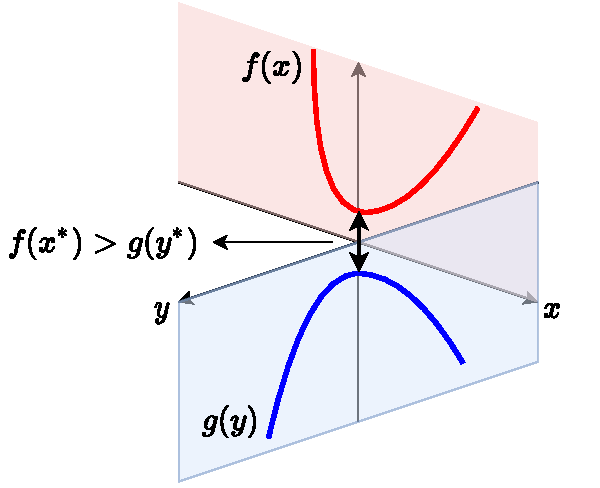
\includegraphics[width=\linewidth]{./figures/weak_dual.pdf}
      \captionsetup{justification=centering}
      \caption{Weak duality.}
    \end{subfigure}
    \hfill
    \begin{subfigure}{.48\textwidth}
      \centering
      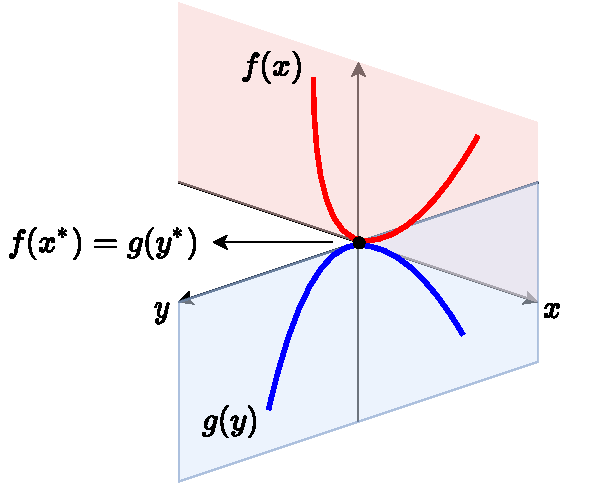
\includegraphics[width=\linewidth]{./figures/strong_dual.pdf}
      \captionsetup{justification=centering}
      \caption{Strong duality.}
    \end{subfigure}
    \captionsetup{justification=centering}
    \caption{Geometric illustration of weak and strong duality.}
    \label{fig:duality}
\end{figure}

\begin{theorem}[Duality theory~\protect{\citep[Theorem~11.39]{rockafellar1998variational}}] Consider the primal-dual pair:~\eqref{prob:general_primal} and~\eqref{prob:general_dual}, where $F: \Re^n \times \Re^m \to \Re$ is a proper, closed and convex function. The following properties hold. 
    \begin{itemize}
        \item \textbf{Weak duality}. The inequality $v_F(0) \geq v_F^{**}(0)$ always holds. 
        \item \textbf{Strong duality}. If $0 \in \ri\dom v_F \cup \ri\dom v_F^{**}$, then $v_F(0) = v_F^{**}(0)$. 
        \item \textbf{Optimal solutions.} If the strong duality holds with finite optimal values, then the following characterizations of the optimal solutions to the primal-dual pair are equivalent
            \begin{align}
                (x^*, 0) &\in \partial F^*(0,y^*); \\
                (0, y^*) &\in \partial F(x^*,0); \\
                v_F(0) = F^*(x^*, 0) &= -F^*(0,y^*) = v_F^{**}(0).
            \end{align}
    \end{itemize}
\end{theorem}

The perturbation function $F$ plays an important role in Fenchel-Rockafellar duality theory. Different choices of the perturbation function will lead to different dual problems. In the rest of this section, we will interpret three widely used primal-dual pairs: Lagrangian dual, Fenchel-Rockafellar dual and gauge dual, under this perturbation framework.  


\subsection{Lagrangian duality}
Consider the general constrained convex optimization problem:
\begin{equation} \label{prob:general_constrained} 
    \minimize{x \in \Re^n} f(x) \st c_i(x) \leq 0 \enspace \forall i = 1, \dots, m,
\end{equation}
where $f:\Re^n\to\Re$ and $c_i:\Re^n\to\Re$ for all $i\in[m]$ are convex functions. In this case, the perturbation function is defined as 
\begin{equation}
    F(x, u) = f(x) + \sum_{i = 1}^m \delta_{\leq 0}(c_i(x) + u_i).
\end{equation}
Then we can derive the corresponding conjugate function as 
\begin{align*}
    -F^*(0, y) &= -\sup_{x\in\Re^n, u\in\Re^m} \ip{0}{x} + \ip{y}{u} - F(x,u)
             \\&= -\sup_{x\in\Re^n, w\in\Re_+^m} \sum_{i=1}^m \ip{y_i}{- c_i(x) - w_i} - f(x)
             \\&= 
             \begin{cases}
                 \inf_{x\in\Re^n} f(x) + \sum_{i=1}^m \ip{y_i}{c_i(x)} & \text{if} y \in\Re_+^m \\
                 -\infty & \text{otherwise}.
             \end{cases}
\end{align*}
Therefore, the Lagrangian dual to problem~\eqref{prob:general_constrained} is given by
\begin{equation} \label{prob:general_constrained_dual}
    \maximize{y\in\Re_+^m} \minimize{x \in \Re^n} f(x) + \sum_{i=1}^m \ip{y_i}{c_i(x)}.
\end{equation}
The following theorem, summarized by \citet{boyd:2004}, characterizes the duality correspondence for the Lagrangian primal-dual pair. 

\begin{theorem}[Lagrangian duality theory~\protect{\citep[Section~5.3]{boyd:2004}}] 
    Let $p^*$ and $d^*$ denote respectively the optimal values for the Lagrangian primal-dual pair:~\eqref{prob:general_constrained} and~\eqref{prob:general_constrained_dual}. 
    \item \textbf{Weak duality}. $p^* \geq d^*$. 
    \item \textbf{Strong duality}. 
    If there exist an interior-point feasible point $\hat x$ for the primal problem~\eqref{prob:general_constrained}, i.e. $c_i(\hat x) < 0$ for $i = 1,\dots,m$, then $p^* = d^*$. Furthermore, let $x^*$ and $y^*$ denote respectively the optimal solutions to the primal-dual pair:~\eqref{prob:general_constrained} and~\eqref{prob:general_constrained_dual}, then 
    \[y_i^*c_i(x^*) = 0 \enspace \forall i = 1,\dots,m.\]
\end{theorem}


\subsection{Fenchel-Rockafellar duality}
Consider the following optimization problem 
\begin{equation} \label{prob:general_fenchel} 
    \minimize{x \in \Re^n} f(x) + g(Mx),
\end{equation}
where $f:\Re^n\to\Re$ and $g:\Re^m\to\Re$ are closed convex functions, and $M:\Re^n\to\Re^m$ is a linear operator. In this case, the perturbation function is defined as 
\begin{equation}
    F(x, u) = f(x) + g(Mx + u).
\end{equation}
Then we can derive the corresponding conjugate function as
\begin{align*}
    -F^*(0, y) &= -\sup_{x\in\Re^n, u\in\Re^m} \ip{0}{x} + \ip{y}{u} - f(x) - g(Mx + u)
             \\&= -\sup_{x\in\Re^n} \left\{\sup_{u\in\Re^m} \ip{y}{Mx + u} - g(Mx + u)\right\} - f(x) - \ip{y}{Mx}
             \\&= - g^*(y) - \sup_{x\in\Re^n}\ip{-M^*y}{x} - f(x) 
             \\&= - g^*(y) - f(-M^*y).
\end{align*}
Therefore, the Fenchel-Rockafellar dual to problem~\eqref{prob:general_fenchel} is given by
\begin{equation} \label{prob:general_fenchel_dual}
    \maximize{y\in\Re^m} - g^*(y) - f(-M^*y).
\end{equation}
The following theorem, developed by \citet{rockafellar1970convex}, characterizes the duality correspondence for the Fenchel-Rockafellar primal-dual pair. 

\begin{theorem}[Fenchel-Rockafellar duality theory~\protect{\citep[Corollary 31.2.1]{rockafellar1970convex}}] 
    Let $p^*$ and $d^*$ denote respectively the optimal values for the Fenchel-Rockafellar primal-dual pair:~\eqref{prob:general_fenchel} and~\eqref{prob:general_fenchel_dual}. 
    \item \textbf{Weak duality}. $p^* \geq d^*$. 
    \item \textbf{Strong duality}. 
    If $0\in\int(\dom g - M\dom f)$, then $p^* = d^*$. Furthermore, let $x^*$ and $y^*$ denote respectively the optimal solutions to the primal-dual pair:~\eqref{prob:general_fenchel} and~\eqref{prob:general_fenchel_dual}, then the following relationships hold
    \begin{align*}
          y^* &\in \partial g(Mx^*) \cap (M^*)^{-1}\partial f(x^*) \tand
        \\x^* &\in \partial f^*(-M^*y^*)\cap M^{-1}\partial g^*(y^*).
    \end{align*}
\end{theorem}




\subsection{Gauge duality}
Consider the following gauge optimization problem 
\begin{equation} \label{prob:general_gauge} 
    \minimize{x \in \Re^n} \gauge\Cs(x) \st Mx = b,
\end{equation}
where $\Cscr\subseteq\Re^n$ is a convex set and $\gauge\Cs$ is the corresponding gauge function, $M:\Re^n\to\Re^m$ is a linear operator, and $b\in\Re^m$ is a vector. By setting 
$\lambda \coloneqq 1/\gauge\Cs(x)$ and $w \coloneqq \lambda x$, problem~\eqref{prob:general_gauge} can be expressed as 
\begin{equation} \label{prob:general_gauge2} 
    \inf_{\lambda > 0, w \in \Re^n} \frac{1}{\lambda} \st w \in \Cscr \tand Mw = \lambda b.
\end{equation}
Note that minimizing $1/\lambda$ is equivalent to minimizing $-\lambda$ for $\lambda \geq 0$. In this case, the perturbation function is defined as 
\begin{equation}
    F(\lambda, w, u) = -\lambda + \delta\Cs(w) + \delta_{\{0\}}(\lambda b - Mw + u) + \delta_{\geq 0}(\lambda). 
\end{equation}
Then we can derive the corresponding conjugate function as
\begin{align*}
    -F^*(0, y) &= -\sup_{\lambda\in\Re, w\in\Re^n, u\in\Re^m} \ip{y}{u} + \lambda - \delta\Cs(w) - \delta_{\{0\}}(\lambda b - Mw + u) - \delta_{\geq 0}(\lambda)
    \\&= -\sup_{\lambda\in\Re, w\in\Re^n} \lambda - \delta\Cs(w) - \delta_{\geq 0}(\lambda) - \ip{\lambda b - Mw}{y}
    \\&= -\sup_{\lambda\geq 0} \delta\Cs^*(M^*y) + \lambda ( 1 - \ip{b}{y} )
    \\&= 
        \begin{cases}
            -\delta\Cs^*(M^*y) & \text{if} \ip{b}{y} \geq 1 \\
            -\infty & \text{otherwise}.
        \end{cases}
\end{align*}
Therefore, the gauge dual to problem~\eqref{prob:general_gauge} is given by
\begin{equation} \label{prob:general_gauge_dual}
    \maximize{y\in\Re^m} -\delta\Cs^*(M^*y) \st \ip{b}{y} \geq 1.
\end{equation}
The following theorem, developed by \citet{friedlander2014gauge}, characterizes the duality correspondence for the gauge primal-dual pair. 

\begin{theorem}[Gauge duality theory~\protect{\citep[Theorem~5.1 and Corollary~5.2]{friedlander2014gauge}}] 
    Let $p^*$ and $d^*$ denote respectively the optimal values for the gauge primal-dual pair:~\eqref{prob:general_gauge} and~\eqref{prob:general_gauge_dual}. 
    \item \textbf{Weak duality}. If both primal problem~\eqref{prob:general_gauge} and dual problem~\eqref{prob:general_gauge_dual} are feasible, then $p^* d^* \geq 1$. 
    \item \textbf{Strong duality}. If either primal problem~\eqref{prob:general_gauge} or dual problem~\eqref{prob:general_gauge_dual} is strictly feasible and the other is feasible, then $p^* d^* = 1$. Furthermore, let $x^*$ and $y^*$ denote respectively the optimal solutions to the primal-dual pair:~\eqref{prob:general_gauge} and~\eqref{prob:general_gauge_dual}, then 
    \[\ip{x^*}{M^*y^*} = \gauge\Cs(x^*)\delta\Cs^*(M^*y^*).\]
    
\end{theorem}

\section{Structured optimization} \label{sec:1-3}

Convex optimization provides a valuable computational framework that renders many problems tractable because of the range of powerful algorithms that can be brought to the task. The key is that a specific mathematical structure, i.e., the convexity of the functions and sets defining the problem—opens an enormous range of theoretical and algorithmic tools that lend themselves astonishingly well to computation. However, there are limits to the scalability of general-purpose algorithms for convex optimization. As has been recognized in the optimization and related communities for at least the past decade, significant efficiencies can be gained by acknowledging the latent structure in the solution itself, coupled with the overarching structure provided by convexity.

Structured optimization proceeds by using a prescribed set of atoms to assemble an optimal solution. The atomic decomposition of a vector $x\in\Re^n$ with respect to an atomic set
$\Ascr\subset\Re^n$ is given by the weighted superposition
\begin{equation} \label{eq:atomic-decomp}
  x = \sum_{a\in\Ascr} c_a a, \quad c_a\ge0 \quad \forall a\in\Ascr.
\end{equation}
Each coefficient $c_a$ in the atomic decomposition measures the contribution of
the corresponding atom $a$ toward the representation of $x$. Intuitively, an
atomic decomposition reveals structural information implicit in a vector, with
large coefficients in the decomposition indicating the more essential
structures.

Within the context of an optimization problem, the atomic decomposition reveals
structural elements most essential in the minimization process.
In the simplest case, the atoms $\Ascr$ may be formed from the collection of
signed canonical unit vectors $\{\pm e_1,\ldots,\pm e_n\}$, which leads to the
atomic decomposition
\[
  x = \sum_{j=1}^n c_j a_j,
  \quad
  c_j: = |x_j|,
  \quad
  a_j:= (\sgn x_j)\cdot e_j.
\]
Trivially, the essential atoms thus correspond to the variables $x_j$ in
the vector $x=(x_1,\ldots,x_n)$ with nonzero magnitude.

This generic model for atomic decompositions was promoted by~\citet{cds98} in the context of sparse signal decomposition, and more recently, by~\citet{chandrasekaran2012convex}, who were concerned with obtaining sparse solutions to linear inverse problems. 

In this thesis, we want to answer the question of determining which of the atoms in the atomic set $\Ascr$ are essential to the atomic decomposition of $x$, and conversely, which atoms can be safely ignored. In \autoref{ch:Dual-Struc-Opt}, we study the atomic decomposition framework from a dual perspective. Polarity, which extends the familiar notion of orthogonality from linear sets to general convex sets, plays a special role in a simple and geometric form of convex duality. This duality correspondence yields a general notion of alignment that leads to an intuitive and complete description of how atoms participate in the final decomposition of the solution. The resulting dual perspective leads to variations of existing algorithms effective for large-scale problems. We illustrate these ideas with many examples, including applications in matrix completion and morphological component analysis. We further show that this dual alignment property allows us to design new structured optimization models for real-world applications and develop efficient and scalable algorithms for structured optimization problems. We briefly introduce the roadmap below. 

In \autoref{ch:App-Sig-Demix}, we study the structured signal demixing problem which seeks to separate a superposition of multiple signals into its constituent structural components. We propose a two-stage approach that first decompresses and subsequently deconvolves the noisy and undersampled observations of the superposition. Probabilistic error bounds are given on the accuracy with which this process approximates the individual signals. The theory of polar convolution of convex sets developed by~\citet{friedlander2019polarconvolution}, and the dual alignment property developed in \autoref{ch:Dual-Struc-Opt} play central roles in the analysis and solution process. If the measurements are random and the noise is bounded, this approach stably recovers low-complexity and mutually incoherent signals, with high probability and with optimal sample complexity. Numerical experiments on both real and synthetic data confirm the theory and the efficiency of the approach.

In \autoref{ch:App-Primal-Retrieval}, we study the structured data-fitting problem, which is prevalent in machine learning and data mining. In practice, people solve the corresponding structured convex relaxations. When tackling high-dimensional structured optimization problems, dual-based algorithms are usually preferred over primal-based algorithms as dual variables usually live in a much lower-dimensional space than primal variables. One common issue of dual-based algorithms is that they still need to translate dual variables to primal variables at some point. How to retrieve a near-optimal primal variable efficiently with a provable guarantee is thus crucial for the success of dual approaches. We present a simple and computationally cheap strategy for retrieving a primal variable from any feasible dual variable, which is based on the dual alignment property developed in \autoref{ch:Dual-Struc-Opt}. Theoretically, we show that our proposed strategy is capable of obtaining a near-optimal primal variable given a dual-based algorithm converging to the optimal dual solution. Numerical experiments on real-world datasets support our analysis.

In \autoref{ch:App-AtomicOpt}, we introduce our open-source package \texttt{AtomicOpt.jl} for solving a class of structured optimization problems, which is written in the Julia programming language~\citep{bezanson2017julia}. Our design depends on the level-set method~\citep{aravkin2016levelset}, a dual version of the conditional-gradient method~\cite{jaggi2013revisiting,frank1956algorithm,dunn1978conditional}, and the primal-retrieval strategy developed in~\autoref{ch:App-Primal-Retrieval}. The worst-case computational complexity of our algorithm is sublinear in the required accuracy. All the numerical experiments conducted in~\autoref{ch:Dual-Struc-Opt},~\autoref{ch:App-Sig-Demix} and~\autoref{ch:App-Primal-Retrieval} are reproducible via this package. 



 

\section{Federated learning} \label{sec:1-4}

With the development of artificial intelligence, people recognize that many powerful machine learning models are driven by large decentralized datasets, e.g., AlphaGo~\citep{silver2016mastering} and AlexNet~\citep{krizhevsky2012imagenet}. In many industry-scale applications, training data is distributed in the form of silos, that is, training data is obtained and maintained by many data owners instead of being centralized at the place of a single owner or a data center. Because of industrial competition, privacy concerns, legal restrictions, and many other possible reasons, integrating or centralizing data from different sources faces enormous resistance and is often even infeasible~\citep{li2020review}. Federated learning, originally proposed by~\citet{federated2016}, is promising for training machine learning models on distributed data sources. It facilitates collaboration among a group of data owners (aka.~``clients'') and, at the same time, preserves their privacy. The central idea of federated learning is to periodically aggregate local models from clients to produce a more general and capable global model.

Federated learning can be further be classified into two main categories: horizontal federated learning and vertical federated learning~\cite{yang2019federated}. Horizontal federated learning refers to the scenarios where various clients' data sets share the same feature space but have separate sample IDs, and vertical federated learning refers to the scenarios where data sets owned by different clients share the identical sample IDs but have distinctive features. A simple characterization is shown in \autoref{fig:hfl_and_vfl}. 

\begin{figure}[t] 
    \begin{subfigure}{.48\textwidth}
      \centering
      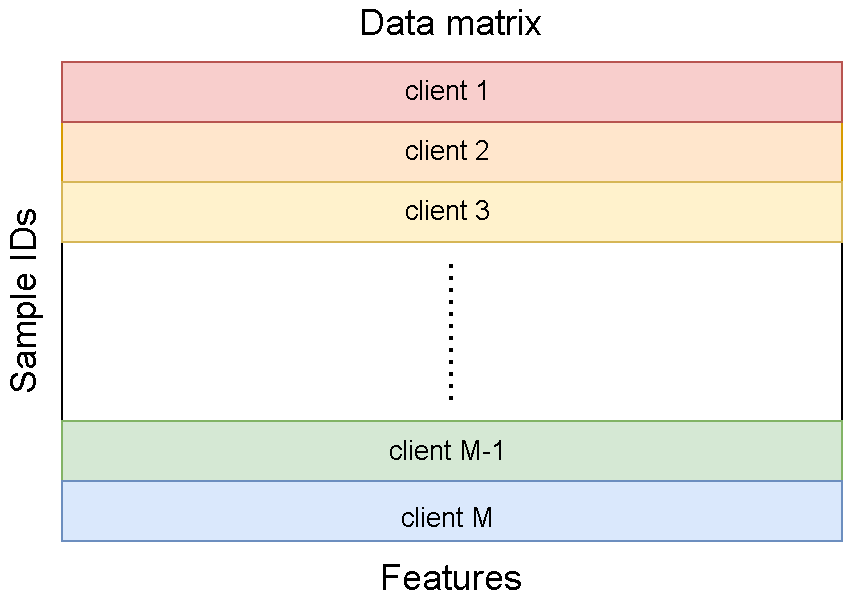
\includegraphics[width=\linewidth]{./figures/hfl_illustration.pdf}
      \captionsetup{justification=centering}
      \caption{Horizontal federated learning.}
      \label{fig:hfl}
    \end{subfigure}
    \hfill
    \begin{subfigure}{.48\textwidth}
      \centering
      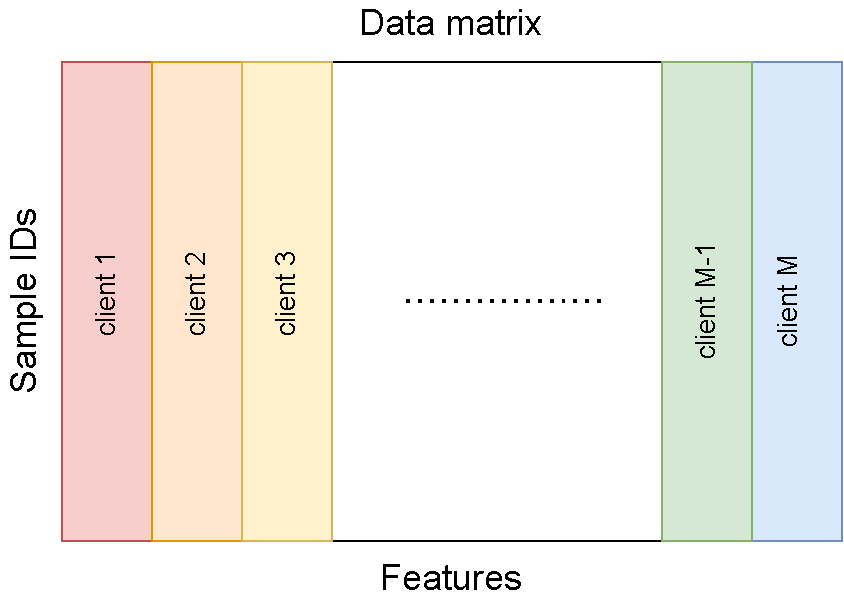
\includegraphics[width=\linewidth]{./figures/vfl_illustration.pdf}
      \captionsetup{justification=centering}
      \caption{Vertical federated learning.}
      \label{fig:vfl}
    \end{subfigure}
    \captionsetup{justification=centering}
    \caption{Characterization of horizontal and vertical federated learning.}
    \label{fig:hfl_and_vfl}
\end{figure}

This thesis shows that duality can be utilized to develop efficient and scalable algorithms for the optimization problem arising from federated learning. Besides, we show that structured optimization techniques can play an essential role in designing fair contribution valuation rules in federated learning. We briefly introduce the roadmap below. 

\subsection{Federated optimization} \label{sec:1-4-1}

A federated learning system is often composed of two components: clients and a central server at the physical level. The learning process in federated learning can be formulated as a distributed optimization problem, also known as federated optimization. As characterized and formalized by~\citet{wang2021field},~\citet{li2020federated} and~\citet{li2019convergence}, several essential characteristics distinguish FO from standard machine learning and distributed optimization. 

\begin{assumption}[Governing assumptions for federated optimization] \label{assum:govern}
The following assumptions hold for federated optimization. 
  \begin{itemize}
    \item \textbf{Slow Communication.}  Communication between clients and a central server is assumed to be the main bottleneck and dominates any computational work done at each of the clients. 
    \item \textbf{Data Privacy.} Clients want to keep their local data private, i.e., their data can not be accessed by any other client nor by the central server.
    \item \textbf{Data heterogeneity.} The training data are not independent and identically distributed (i.i.d.). In other words, a client’s local data cannot be regarded as samples drawn from single overall distribution.
    \item \textbf{Partial Participation.} Unlike traditional distributed learning systems, an FL system does not have control over individual client devices, and clients may have limited availability for connection. 
\end{itemize}
\end{assumption}

In \autoref{ch:Dual-Fed-Opt}, we study the federated optimization problem from a dual perspective. We propose a new algorithm termed federated dual coordinate descent (FedDCD), which is based on a type of coordinate descent method developed by \citet{necoara2017random}.  Additionally, we
enhance the FedDCD method with inexact gradient oracles and Nesterov's acceleration. We demonstrate
theoretically that our proposed approach achieves better convergence rates than the state-of-the-art
primal federated optimization algorithms under certain situations. Numerical experiments on real-world
datasets support our analysis.

\subsection{Contribution valuation in federated learning} \label{sec:1-4-2}

The effectiveness of federated learning depends on the active participation of motivated clients. Another important question in federated learning is how to ensure the clients’ long-term engagement, and how to motivate more clients' participation. One possible practical solution is to recompense the participated clients according to their contribution. 

Shapley value~\cite{shapley201617} is a classical measure originates from cooperative game theory to fairly assess contributions by participants in a coalition. 
The Shapley value of a participant is defined as the expectation of the marginal contribution of the participant over all possible subsets of the other participants. Shapley value is the unique measure that satisfies the four fundamental requirements of fairness proposed by Shapley~\cite{shapley201617}: balance, symmetry, zero element and additivity, which we formally define bellow. 

\begin{definition} \label{def:shapley}
    Supporse there are $M$ clients and there is a black-box utility function $U:2^{[M]} \to \Re$ such that for any subset of clients $S \subseteq [M]$, the function $U(S)$ returns a utility score of the model collaboratively trained by the clients in $S$, such as the performance of the model. Let $v: [M] \to \mathbb{R}$ be the evaluation metric associated with the utility function $U$. The metric $v$ is called \emph{Shapley-fair} with respect to $U$ if it satisfies the following for fundamental requirements
    \begin{enumerate}
        \item \textbf{Symmetry.} For any two clients $i, j \in [M]$, if for any subset of clients $S \subseteq [M] \setminus \{i,j\}$, $U(S \cup \{i\}) = U(S \cup \{j\})$, then $v(i) = v(j)$. 
        \item \textbf{Zero element.} For any client $i \in [N]$, if for any subset of clients $S \subseteq [M] \setminus \{i\}$, $U(S \cup \{i\}) = U(S)$, then $v(i) = 0$.
        \item \textbf{Additivity.} If the utility function $U$ can be expressed as the sum of separate utility functions, namely $U = U_1 + U_2$ for some $U_1, U_2 : 2^I \to \mathbb{R}$, then for any client $i \in [M]$, $v(i) = v_1(i) + v_2(i)$, where $v_i$ and $v_2$ are the evaluation metrics associated with the utility functions $U_1$ and $U_2$, respectively. 
        \item \textbf{Balance.}  $U([M]) = \sum_{i \in [M]} v(i)$.
    \end{enumerate}
\end{definition}

Under the federated learning setting, a utility function is usually defined as the model performance on a data set. The symmetry requires that the same contributions to the performance should receive the same evaluation, which implies that clients with same local data sets should receive same evaluation. The zero element requires that no contribution, no value is recognized. The additivity requires that if there are multiple tasks and thus multiple test data sets, then the contributions of any client with respect to the test data sets can be expressed as the sum of the contributions with respect to those different tasks and test data sets. Note that, although balance is a necessary condition in many economic contests because it ensures payment is fully distributed to all clients, it is irrelevant in the context of federated learning because we are only concerned about the relative contributions of clients. It is shown~\cite{dubey1975uniqueness,ghorbani2019data} that if the data valuation metric $v$ satisfies symmetry, zero element, and additivity, then $v$ must have the form
\begin{equation} \label{eq:shapley}
    v(i) = c \sum\limits_{S \subseteq I \setminus\{i\}} \frac{1}{\binom{N-1}{|S|}} \left[U(S\cup\{i\}) - U(S)\right],
\end{equation}
for some positive constant $c$.  

Although Shapley value has many desirable properties, evaluating Shapley value in federated learning requires exhaustive retraining and evaluating the model on every subset of clients. The costs of communication and time may be prohibitive in practice~\cite{song2019profit}. To tackle this challenge, some variations inspired by Shapley value were developed. Federated Shapley value (FedSV), recently proposed by \citet{wang2020principled}, is a measure for valuating contribution under the framework of horizontal federated learning. The key idea is to compute the Shapley values for clients in each round of training and then report the summation over all the rounds as the final results. This design cleverly avoids model retraining. However, there are still factors of potential unfairness in the design of FedSV because two data owners with the same local data may not receive the same evaluation. 

In \autoref{ch:Val-HFL}, we propose a new measure called completed federated Shapley value (ComFedSV) for contribution valuation in horizontal federated learning, which improves the fairness of FedSV. The design depends on completing a matrix consisting of all the possible contributions by different subsets of the data owners. It is shown under mild conditions that this matrix is approximately low-rank by leveraging concepts and tools from structured optimization. Both theoretical analysis and empirical evaluation verify that the proposed measure does improve fairness in many circumstances.

In \autoref{ch:Val-VFL}, we extend the idea of FedSV to vertical federated learning. We propose a contribution valuation metric called vertical federated Shapley value (VerFedSV), which utilizes tools from structured optimization. We show that VerFedSV not only satisfies many desirable properties for fairness but is also efficient to compute, and can be adapted to both synchronous and asynchronous vertical federated learning algorithms. Both theoretical analysis and extensive experimental results verify the fairness, efficiency, and adaptability of VerFedSV.






%    2. Duality in structured optimization
%% The following is a directive for TeXShop to indicate the main file
%%!TEX root = diss.tex
\chapter{Duality in structured optimization}
\label{ch:Dual-Struc-Opt}

\section{Background}
As we introduced in \autoref{sec:struc-opt}, structured optimization uses a prescribed set of atoms to assemble a solution that fits a model to data. Our purpose with this chapter is to describe the rich convex geometry and the duality that
underlies atomic decomposition. The path we follow builds on the duality
inherent in convex cones: every convex cone is paired uniquely with another cone that is polar to it. The extreme rays of each cone in this pair are in some sense \emph{aligned}. Brought into the context of atomic decomposition, this
notion of alignment through the polar operation provides a theoretical framework
that can be harnessed to identify the atoms that participate in a decomposition. This
approach facilitates certain algorithmic design patterns that promote
computational efficiency, as we demonstrate with concrete examples. Similar
computational economies accrue within reduced-space active-set methods for
optimization problems with inequality constraints, such as implemented by the
MINOS software package \citep{murtsaun:1983}.

Early work in structured optimization focused on problem formulations meant to
produce sparse solution vectors, i.e., a solution with relatively few non-zero
elements. Compressed sensing \cite{cds98,chendonosaun:2001,crt06a} and model
selection \cite{tibshirani1996regression,tibshirani1997lasso} , with their many applications
in signal processing and statistics, helped to establish sparse optimization as
an important class of problems with a range of specialized algorithms.
Generalizations that accommodated different notions of sparsity soon followed,
including matrix problems with low-rank solutions (sparsity in the vector of
singular values), fused index pairs (sparsity in terms of the norms of subgroups of variables), and sparsity in specialized dictionaries, such as mass
spectrographs of simple molecules used to represent structures of
more complicated molecules \cite[Section~6.3.1]{vandenberghe:2010}.

Nonsmooth regularization functions that promote sparsity, such as the 1-norm for
sparse vectors, or the nuclear norm for low-rank matrices, are key features of
these formulations. Gauge functions, which significantly generalize the notion
of a norm, were recognized as flexible regularization functions that promote a
broad range of sparse structures. By defining a set of atoms from which to build
a solution, an almost arbitrary set of solution structures can be considered.
The gauge function to this set can be incorporated into a convex optimization
problem in order to obtain a solution with the desired structure. The convex
analysis of gauges and support functions, which are their dual counterparts, is
rich in geometry and rife with opportunity for efficient algorithm
implementations for high-dimensional problems. Our purpose with this monograph
is to expose the basic elements of this theory and its many connections to
sparse and structured optimization. To make it accessible researchers who are
not specialists in convex analysis, we chose a largely self-contained treatment
and make a few modest assumptions that greatly simplify the derivations.

\subsection{Applications and prior work}

One of the main implications of our approach is its usefulness in using dual
optimization methods for discovering atomic decompositions. With the tools of
polar alignment, a dual optimization method can be interpreted as solving for an
aligning dual vector $z$ that exposes the support of a primal solution $x$. If
the number of exposed atoms is small, a solution $x$ of the primal problem can
be obtained from a reduced problem defined over the exposed support, but without
the nonsmooth atomic regularization. The resulting reduced problem is often
computationally much cheaper~\citep{freund2017extended} and better
conditioned~\citep{negahban2012restricted}. Alternatively, two-metric methods can
be designed to act differently on a primal iterate's suspected
support~\citep{gafni1984two}. In many applications, such as feature selection,
knowing the optimal support may itself be sufficient.  As we illustrate through
various examples, there are several important cases where the dual aligning
vector $z$ can be computed directly.

\paragraph{Machine learning}

The regularized optimization problems described in \autoref{sec:manifestations}
frequently appear in applications of machine learning for the purpose of model
complexity reduction. The most popular tools are the vector 1-norm in feature
selection~\cite{tibshirani1996regression}, its group-norm
variant~\cite{jacob2009group}, and the nuclear norm in matrix completion
\cite{recht2010guaranteed}. 
Many other sparsity-promoting regularizers, however,
appear in practice \cite{zeng2014ordered}. Although unconstrained formulations
are most popular, particularly when the proximal operator is computationally
convenient~\cite{parikh2013proximal}, the gauge-constrained formulation is
frequently used and solved via the conditional gradient method
\cite{frank1956algorithm,dunn1978conditional,jaggi2013revisiting}. Popular dual
methods, which iterate over a dual variable $z^{(k)}$ but maintain the
corresponding primal variable $x^{(k)}$ only implicitly, include bundle methods
\cite{lemarechal1981bundle} and dual averaging
\citep{xiao2010dual,duchi2012dual}.

\paragraph{Linear conic optimization}

Conic programs are a cornerstone of convex optimization. The nonnegative cone,
the second-order cone and the semidefinite cone respectively, give rise to
linear, second-order, and semidefinite programs. These problem classes capture
an enormous range of important models, and can be solved efficiently by a
variety of algorithms, including interior methods
\cite{karmarkar1984new,nen94,rene:2001}. Conic programs and their associated
solvers are key ingredients for general purpose optimization software packages
such as YALMIP~\citep{lofberg2004yalmip} and CVX~\cite{grant2008cvx}. The
alignment conditions for these specific cones have been exploited in dual
methods, such as in the spectral bundle method for large-scale semidefinite
programming \cite{helmberg2000spectral}. \autoref{example-conic-opt} demonstrates
this alignment principle in the context of conic optimization.

\paragraph{Gauge optimization} 

The class of gauge optimization problems, as defined by Freund's 1987 seminal
work~\citep{freund1987dual}, can be simply stated: find the element of a convex
set that is minimal with respect to a gauge function. These conceptually simple
problems appear in a remarkable array of applications, and include parts of
sparse optimization and all of conic
optimization~\cite[Example~1.3]{friedlander2014gauge}. This class of
optimization problems admits a duality relationship different from classical
Lagrange duality, and is founded on the polar inequality.
In this context, the polar inequality provides an analogue to weak duality,
well-known in Lagrange duality, which guarantees that any
feasible primal value provides an upper bound for any feasible dual
value. In the gauge optimization context, a primal-dual pair $(x,z)$ is optimal
if and only if the polar inequality holds as an equation, which under
\autoref{def:alignment} implies that $x$ and $z$ are
aligned. 
The connection between polar alignment and optimality is
discussed further in \autoref{sec:gauge-optimization}.

\paragraph{Two-stage methods}
In sparse optimization, two-stage methods first identify the primal variable
support, and then solve the problem over a reduced support
\cite{ko1994iterative,cristofari2017two}. If the support is sparse enough, the
second problem may be computationally much cheaper, either because it allows for
faster Newton-like methods, or because of better conditioning
\cite{negahban2012restricted}. The atomic alignment principles we describe in
\autoref{sec:convexanalysis-atomic} give a general recipe for extracting primal
variable support from a computed dual variable, which at optimality is aligned
with the primal variable; see \autoref{sec:manifestations}. 

\paragraph{Method interpretability}
The connection between sparsity and alignment points to a likely ``aligning
behavior" in many of the most effective methods for sparse
optimization~\cite{hare2004identifying}. Indeed, we show in \autoref{sec:methods}
that this is true for a range of methods, including proximal gradient,
conditional gradient, and cutting plane methods. Surprisingly, we also find
hints of aligning behavior in seemingly unrelated methods, such as augmented
Lagrangian and bundle methods. The alignment point of view thus offers greater
interpretability of commonly used methods in many modern optimization
applications.

\section{Atomic decomposition} \label{sec:atomic-decomposition}
Recall the atomic decomposition of a vector $x\in\Re^n$ with respect to an atomic set $\Ascr\subseteq\Re^n$; see \eqref{eq:atomic-decomp}. We are particularly interested in the question of determining which of the atoms
in $\Ascr$ are essential to the atomic decomposition of $x$, and conversely,
which atoms can be safely ignored. 

\subsection{Gauge functions reveal the atomic support}
The following equivalent expression of the gauge function 
\begin{equation}
    \label{eq:gauge2}
    \gauge\As(x)
    = \inf_{c_a}
      \left\{ \sum_{a\in\Ascr}c_a ~\bigg\vert~ x = \sum_{a\in\Ascr}c_aa,\ c_a \ge0\ \forall a\in\Ascr \right\},
\end{equation}
helps to define the answer to the question above; cf.~\autoref{prop-guage-equivalence}. This function returns the
minimal sum of weights over all valid atomic decompositions of $x$ with respect
to the set $\Ascr$. The value $\gauge\As(x)=\infty$ indicates that there doesn't
exist a valid atomic decomposition for $x$. (For example, an atomic set composed
of nonnegative vectors cannot decompose a vector~$x$ that contains negative entries.) 

In the framework outlined by \citet{chandrasekaran2012convex}, the gauge
function $\gauge\As$ defines the objective of a convex optimization problem
suitable for recovering a signal from a small number of partial observations. In
that context, the number of atoms needed to decompose the signal determines the
number of observations needed to reconstruct the signal.

The significant atoms---those that \emph{support} the
vector $x$---are those that contribute positively in forming the minimal sum. We
are thus led to the following definition.

\begin{definition}[Atomic support] \label{def:support} A subset of atoms
    $\suppa(x)\subset\Ascr$ is a \emph{support set} for $x$ with respect to
    $\Ascr$ if every atom $a\in\suppa(x)$ has a strictly positive coefficient
    $c_a$ in the atomic decomposition~\eqref{eq:atomic-decomp}. That is,
    \begin{equation}
      \label{eq:support}
      \gauge\As(x) = \sum_{\mathclap{a\in\suppa(x)}} c_a,
      \qquad x = \sum_{\mathclap{a\in\suppa(x)}} c_aa,
      \text{and} c_a > 0\enspace \forall a\in\suppa(x).
    \end{equation}
    The set $\supp\As(x)$ is defined as the set of all support
    sets. Thus, any set in $\supp\As(x)$ is a valid support set. 
  \end{definition}

\subsection{Polar inequality} \label{sec:approach}

How do we identify the support of a vector $x$ with respect to an arbitrary
atomic set $\Ascr$? The direct approach requires us to solve the minimum-weight
problem defined by the gauge~\eqref{eq:gauge2}, and determine a valid decomposition
from the positive elements of the computed solution. Thus, to identify all
possible atomic support sets, we need to compute all possible solutions
to~\eqref{eq:gauge2}. As we will demonstrate, however, a complete description of all
possible solution sets can be obtained using the concept of \emph{polar
alignment}, which we define in this section. Our approach is based on a certain
duality correspondence particular to gauge functions and to convex cones that
are implicit in their definition. We describe in \autoref{sec:convexanalysis} this correspondence and its relationship to atomic decompositions. Here we give only the basic elements needed to define the notion of alignment. The next proposition shows the close relationship between the gauge function and the support function. 

\begin{proposition}[Polar inequality] \label{prop:polar-inequality}
    For all pairs of vectors $(x,z)\in\dom\gauge\As\times\dom\sigma\As$,
    \begin{equation}
      \label{eq:polar-inequality}
      \ip x z \le \gauge\As(x)\cdot\sigma\As(z).
    \end{equation}
\end{proposition}

\begin{figure}[t] 
    \centering
    \includegraphics[page=10]{./figures/illustrations.pdf}
    \caption{%
    An illustration of the proof of the polar
    inequality given by \autoref{prop:polar-inequality}. The inner-product of the scaled vector $\hat x = x/\gauge\As(x)$ with $z$ always lies in the left halfspace defined by
    $\sigma\As(z)$, i.e., $\ip{\hat x}{z}\leq\sigma\As(z)$.
    }
    \label{fig:polar-inequality}
\end{figure}

\begin{proof}
    The proof for the polar inequality in
    \cite[Section~15]{rockafellar1970convex} relies on the polarity of cones.
    Here we provide an elementary proof that only depends on the provided
    definitions of gauge and support functions. First, consider the case
    $\gauge\As(x) > 0$. Let $\xhat=x/\gauge\As(x)$. Thus, $\xhat\in\convA$, and
    \[
      \ip{x}{z} = \gauge\As(x)\cdot\ip{\xhat}{z} \leq \gauge\As(x)\cdot\sigma\As(z),
    \]
    where the inequality follows from the maximality property of the support
  function; see \autoref{fig:polar-inequality}. Next, consider the case $\gauge\As(x)
  = 0$, and proceed by contradiction. Suppose $\ip{x}{z} > 0$. Because
  $\gauge\As(x) = 0$ implies $\lambda x \in \convA$ for all $\lambda > 0$, it
  follows from the positive homogeneity of $\sigma\As$ that $\sigma\As(z) =
  \infty$. This contradicts the assumption that $z \in \dom\sigma\As$. Thus, 
  \[
     \ip{x}{z} \leq 0 = \gauge\As(x)\cdot\sigma\As(z).
  \]
\end{proof}

\begin{example}[Norms] \label{ex:norms}
    When $\Ascr=\{x|\|x\|\le1\}$ is the unit level set to any norm,
  $\|\cdot\|:\Real^n\to\Real_+$, then
  \[
    \gauge\As(x) = \|x\|
    \text{and}
    \sigma\As(z) = \|z\|_d,
  \]
  where $\|\cdot\|_d$ is the dual norm. The polar inequality then reduces to the
  standard inequality between inner products and dual pairs of norms:
  \[
    \ip x z \le \|x\|\cdot \|z\|_d. 
  \]
\end{example}

\subsection{Alignment and support identification}

The polar inequality motivates the following generalized definition of aligned
pairs of vectors.
\begin{definition}[Alignment] \label{def:alignment} A pair
  $(x,z)\in\Real^n\times\Real^n$ is \emph{aligned} with respect to the atomic
  set $\Ascr$, i.e., $x$ and $z$ are $\Ascr$-aligned, if the polar
  inequality~\eqref{eq:polar-inequality} holds as an equation.
\end{definition}

This general notion of alignment follows from the special case where
$\Ascr=\{x|\norm{x}_2 \leq 1\}$ is the unit 2-norm ball. In this case, it follows
from \autoref{ex:norms} that the polar inequality reduces the Cauchy-Schwartz inequality
\begin{equation*}
  \label{eq:cauchy-inequality}
  \ip x z \le \norm{x}_2\cdot\norm{z}_2.
\end{equation*}
This inequality holds as an equation if and only if $x$ and $z$ are aligned in
the usual sense: there exists a nonnegative scalar $\alpha$ such that
$x=\alpha z$. The more general notion of alignment captures other important special
cases, including the H\"older inequality, which is a
special case of~\eqref{eq:polar-inequality} in which $\Ascr$ is the unit
$p$-norm ball, with $p\in[1,\infty]$.

A rich convex geometry underlies this general notion of alignment, and plays a
role in identifying the atoms important for the decomposition~\eqref{eq:atomic-decomp}.
Suppose that a vector $z$ is $\Ascr$-aligned with $x$. As we demonstrate
in \autoref{prop:support-identification}, all atoms $a\in\Ascr$ in the atomic support 
of $x$ must also be $\Ascr$-aligned with $z$, i.e.,
\begin{equation} \label{eq:exposed-atoms}
  \suppa(x)\subseteq\Escr\As(z):=\{a\in\Ascr\cup\{0\} | \ip a z = \sigma\As(z) \}.
\end{equation}
To see that $\Escr\As(z)$ indeed contains all the atoms that are $\Ascr$-aligned
with $z$, note that any atom $a\in\Escr\As(z)$ necessarily has unit gauge value,
i.e., $\gauge\As(a)=1$, which follows from 
\autoref{prop:polar-inequality}. Thus the condition $\ip a z = \sigma\As(z)$
implies that $a$ is $\Ascr$-aligned with $z$. \autoref{fig:essential-atoms}
presents a visualization of this concept. The atoms in $\Escr\As(z)$ are said to
be \emph{exposed} by the vector $z$. As we show in \autoref{sec:exposed-faces},
this set of atoms is contained in the face of $\convA$ exposed by the vector
$z$.

\begin{figure}[t]
    \centering
    \includegraphics[page=4]{./figures/illustrations}
    \caption{The set of atoms in the set $\Ascr$ generally (but not necessarily)
      defines the boundary of the convex hull $\convA$. The set of exposed atoms
      $\Escr\As(z)$ are contained within the supporting hyperplane $\{a|\ip{a}{z}
      =\sigma\As(z)\}$ normal to $z$. The atom $a_1$ is exposed by $z_1$ and all
      other directions that lie in the shaded cone; the atom $a_2$ is exposed by
      the unique direction along $z_2$; and the set of atoms
      $\{a_{3i}\}_{i=1}^3$ are exposed by the unique direction along $z_3$. }
    \label{fig:essential-atoms}
 \end{figure}


\subsection{Examples}

There are many varieties of atomic sets and recognizable convex
regularizers used to obtain sparse decompositions.
\citet{chandrasekaran2012convex} and
\citet{jaggi2013revisiting} both give extensive lists of atoms
and the norms that they induce, as well as their applications in practice.
Here we provide several simple examples that illustrate the variety of
ways in which vectors can be aligned.

\begin{example}[One norm] \label{example-one-norm} Let
    \[\Ascr = \{\pm e_1,\ldots,\pm e_n\}\] be the signed standard basis vectors.
    The gauge to this atomic set induces the 1-norm, which is the canonical
    example of a sparsifying convex penalty. The corresponding support function is
    the dual $\infty$-norm:
    \[
      \gauge\As(x) = \|x\|_1 \text{and} \sigma\As(z) = \|z\|_\infty.
    \]
    The polar inequality~\eqref{eq:polar-inequality} reduces to
    H\"older's inequality for these norms---i.e.,
    $\ip x z \le \|x\|_1\cdot\|z\|_\infty$. As is well known, this holds
    with equality---and thus $x$ and $z$ are $\Ascr$-aligned---if and only
    if
  \begin{equation*}
    x_i \neq 0
    \quad\Longrightarrow\quad
    \sgn(x_i) z_i = \max_j\,|z_j| \quad \forall i=1:n.
  \end{equation*}
  Alignment of the pair $(x,z)$ with respect to the atomic set $\Ascr$ is hence
  equivalent to the statement that $\suppa(x)\subseteq\Escr_\Ascr(z)$, where the
  atomic support for $x$ and the atoms exposed by $z$, respectively, are given the
  the sets
  \begin{align*}
    \suppa(x) &= \{\sgn(x_i)\cdot e_i | x_i \neq 0\},
  \\\Escr_\Ascr(z) &= \{\sgn(z_i)\cdot e_i | |z_i| =  \max_j\,|z_j| \}.
  \end{align*}
  
  The inclusion $\suppa(x)\subseteq\Escr_\Ascr(z)$ also characterizes an
  optimality condition. For example, consider the LASSO~\cite{tibshirani1997lasso}
  problem
  \begin{equation*}
    \minimize{x}\enspace \half\|Ax-b\|_2^2 \enspace\st\enspace\|x\|_1\le\tau,
  \end{equation*}
  where $\tau$ is a positive parameter. It's straightforward to verify that
  $x$ is optimal for this problem if and only if
  $\suppa(x)\subseteq\Escr_\Ascr(z)$ where $z:=A\T(b-Ax)$ is the negative gradient
  of the objective. \autoref{sec:manifestations} describes in detail the
  connection between optimality and alignment.
  \end{example}

  \begin{example}[Nuclear norm] \label{example-nuclear-norm}

    The nuclear norm, or Schatten 1-norm, of a matrix is the spectral analog to
    the vector 1-norm. The nuclear norm and its dual spectral norm can be obtained
    via the atomic set 
    \[
      \Ascr = \{uv^T | \|u\|_2=\|v\|_2 = 1\}
    \]
    of normalized $n$-by-$m$ rank-1 matrices. Let $X$ and $Z$ both be $m$-by-$n$
    matrices with singular values $c_1\ge\cdots\ge c_{m\wedge n}\ge0$ and
    $s_1\ge\cdots\ge s_{m\wedge n}\ge0$, where $m\wedge n:=\min\{m,\, n\}$. The
    corresponding gauge for $X$ is the nuclear norm
    \[
      \gauge\As(X) = \|X\|_1 := \sum_{i=1}^{m\wedge n}c_i,
    \]
    and the support function for $Z$ is the Schatten 2-norm
    \[
       \sigma\As(Z) = \|Z\|_\infty:=\max_{i=1:m\wedge n}s_i.
    \]
    The atomic description of these functions is consistent with the notion that
    the nuclear norm is a convex function that promotes low rank (e.g., sparsity
    with respect to rank-1 matrices) \cite{recht2010guaranteed}. The alignment
    condition $\ip X Z = \norm{X}_1\cdot \norm{Z}_\infty$ holds when $X$ and $Z$
    have a simultaneously ordered singular value decomposition (SVD). Suppose,
    then, that $X$ has rank $r$ and that the largest singular value of $Z$ has
    multiplicity~$d$. If the SVDs of $X$ and $Z$ are
    \[
      X = \sum_{i=1}^r c^{}_i u^{}_iv_i^T
      \text{and}
      Z = \sum_{i=1}^{\mathclap{m\wedge n}} s^{}_iu^{}_iv_i^T,
    \]
    then the atomic support of $X$ is
    \[
      \suppa(X)=\{u^{}_1v_1^T,\ldots,u^{}_rv_r^T\},
     \]
    and the set of atoms exposed by $Z$ is
    \[
      \Escr\As(Z)=\{u^{}_1v_1^T,\ldots,u^{}_dv_d^T\}.
    \]
    The inclusion~\eqref{eq:exposed-atoms}, which identifies the support as a subset of the
    exposed atoms, implies $d \geq r$. Thus, the singular vectors of $Z$
    corresponding to the $d$ singular values $s_1,\ldots,s_d$ contain the singular
    vectors of $X$. Note that this can also be proven as a consequence of von
    Neumann's trace inequality \cite{vonneumann:1937,lewis:1995}.
    \citet{friedlander2016low} use this property for the construction of
    space-efficient dual methods for low-rank semidefinite optimization.
  \end{example}

  \begin{example}[Linear subspaces] \label{example-linear-subspaces}

    Suppose that the set of atoms $\Ascr$ contains all the elements of a
    linear subspace $\Lscr$. In this case, the gauge $\gamma_\Lscr(x)$
    is finite only if $x$ is in $\Lscr$, and similarly, the support
    function $\sigma_\Lscr(z)$ is finite only if $z$ is in its
    orthogonal complement $\Lscr^\perp$. In particular, because $\Lscr$ and
    $\Lscr^\perp$ are cones,
    \[
      \gauge_\Lscr(x) = \delta_\Lscr(x)
      \text{and}
      \sigma_\Lscr(z) = \delta_{\Lscr^\perp}(z).
    \]
  The respective domains of the
    gauge and support functions are thus $\Lscr$ and $\Lscr^\perp$. It
    follows that, under the atomic set $\Lscr$, the vectors $x$ and $z$ are
    $\Lscr$-aligned if and only if $x\in\Lscr$ and $z\in\Lscr^\perp$. Thus, the aligned
    vectors are orthogonal.
  \end{example}
  

\section{Alignment with respect to general convex sets} \label{sec:convexanalysis}

The alignment principles we develop depend on basic notions of convex sets and
their supporting hyperplanes. Gauge and support functions are central because
they furnish a complete and convenient calculus for manipulating and
interpreting atomic sets. The following blanket assumption, which holds
throughout the paper, ensures a desirable symmetry between a set and its polar,
as explained in~\autoref{sec:polarity}. This assumption considerably simplifies our
analysis and fortunately holds for many of the most important and relevant
examples.
\begin{assumption}[Origin containment] \label{blanket-assumption} The set
  $\Cscr\subset\Re^n$ is closed convex and contains the origin.
\end{assumption}

\subsection{Polarity} \label{sec:polarity}

Our notion of alignment is based on the polarity of convex sets. Polarity is
most intuitive in the context of convex cones, which are convex sets closed
under positive scaling: the set $\Kscr$ is a convex cone if
$\alpha\Kscr\subset\Kscr$ for all positive $\alpha$ and $\Kscr + \Kscr \subset
\Kscr$. Its polar
\begin{equation} \label{eq-polar-cone}
  \Kscr\polar=\{z | \ip x z \le 0 \ \forall x\in\Kscr\}
\end{equation}
is also a convex cone, and its vectors make an oblique angle (i.e., a
nonpositive inner product) with every vector in $\Kscr$. The definition of the
polar operation for general convex set $\Cscr$ is similar, except that the 0
bound is replaced with a 1:
\begin{equation} \label{eq-polar-set}
  \Cscr\polar=\{z | \ip x z \le 1 \mbox{\ for all\ } x\in\Cscr \}.
\end{equation}

One way to connect the two polarity definitions~\eqref{eq-polar-cone}
and~\eqref{eq-polar-set} is by ``lifting'' the set $\Cscr$ and its polar
$\Cscr\polar$ and embedding them into slices of the $1$ and $-1$ level sets of the
opposing cones in $\Re^{n+1}$:
\[
  \Kscr\Cs \defd \cone(\Cscr\times\{1\})
  \text{and}
  \Kscr\Cs\polar \defd \cone(\Cscr\polar\times\{-1\}).
\]
Then for any nonzero $(n+1)$-vectors $\xbar\in\Kscr\Cs$ and $\zbar\in\Kscr\Cs\polar$,
there exist positive scalars $\alpha_x$ and $\alpha_z$, and vectors $x\in\Cscr$
and $z\in\Cscr\polar$, such that
\begin{equation} \label{eq:10} 
\begin{aligned}
  \ip\xbar\zbar
    &= \ip*{\alpha_x\pmat{x\\1}}{\,\alpha_z\pmat{\phantom-z\\-1}}
  \\&= (\alpha_x\,\alpha_z)\cdot(\ip x z - 1)
  \\&\le0,
\end{aligned}
\end{equation}
where the last inequality follows from the polar definition in
\eqref{eq-polar-set}. The last inequality in~\eqref{eq:10}  confirms that the
cones $\Kscr\Cs$ and $\Kscr\Cs\polar$ are polar to each other under
definition~\eqref{eq-polar-cone}.

The blanket \autoref{blanket-assumption}, which asserts $\Cscr$ is closed and
contains the origin, yields a special symmetry because then the polar
$\Cscr\polar$ also contains the origin and $\Cscr^{\circ\circ}=\Cscr$
\cite[Theorem~14.5]{rockafellar1970convex}. This is one of the reasons why we
define $\convA=\conv(\Ascr\cup\{0\})$ to include the origin.

The pair of polar sets $\Cscr$ and $\Cscr\polar$ can be said to generate the
corresponding gauge and support functions $\gauge\Cs$ and $\sigma\Cs$, as we
show below. Because the gauge and support functions are positively
homogeneous, the epigraphs for these functions
are convex cones. Moreover, it is straightforward to verify from the Minkowski
characterization of the gauge~\autoref{def:gauge}) and the definition of the polar that
the unit level sets for $\gauge\Cs$ and $\sigma\Cs$ are the sets that define
them:
\begin{equation} \label{eq:15}
  \Cscr=\{x|\gauge\Cs(x)\le1\}
  \text{and}
  \Cscr\polar = \{z|\sigma\Cs(z)\le1\}.
\end{equation}
It thus follows that
\begin{equation}\label{eq:26} 
  \epi\gauge\Cs = \cone(\Cscr\times\{1\})
  \text{and}
  \epi\sigma\Cs = \cone(\Cscr\polar\times\{1\}).
\end{equation}
\autoref{fig:gauge-epi} shows a visualization of the epigraph of the gauge to $\Cscr$.

\begin{figure}[t]
    \centering
    \includegraphics[page=7]{./figures/illustrations}
    \caption{The epigraph of the gauge $\gauge\Cs$ is the cone in
      $\Re^n\times\Real$ generated by the set $\Cscr\subset\Re^n$; see~\eqref{eq:26}.}
    \label{fig:gauge-epi}
  \end{figure}

The recession cone (also known as the asymptotic cone) of a set $\Cscr$ contains
the set of directions in which the set is unbounded:
\begin{equation} \label{eq-recession-cone}
  \rec \Cscr :=
  \{d | \mbox{$x+\lambda d \in \Cscr$ for every $\lambda\ge0$ and $x\in\Cscr$}\}.
\end{equation}
See~\autoref{fig-recession-example} for an illustration.
Vectors in the recession cone can also be thought of as ``horizon
points'' of $\Cscr$ \cite[p.~60]{rockafellar1970convex}. With respect
to the gauge and support functions to the set $\Cscr$, vectors
$u\in\rec\Cscr$ have the property that $\gauge\Cs(u) = 0$ and
$\sigma\Cs(u) = +\infty$; see \autoref{prop-support-properties}. We must
therefore be prepared to consider cases where these functions can take
on infinite values. Far from being a nuisance, this property is useful
in modelling important cases in optimization.

\begin{figure}[t]
  \centering
  \begin{tabular}{@{}c@{\hspace{.5in}}c@{}}
    \includegraphics[page=2]{./figures/illustrations}
    & \includegraphics[page=3]{./figures/illustrations}
      \end{tabular}
      \caption{The contours of the gauge function of $\Cscr$ (left)
        and of $\Cscr\polar$ (right). All vectors $x$ in the recession
        cone of $\Cscr$ have gauge value $\gauge\Cs(x)=0$. A vector
        $x_1$ can only be $\Cscr$-aligned with another vector $z_1$ if
        they are orthogonal to each and each is an extreme ray,
        respectively, of $\rec\Cscr$ and
        $\dom\gamma\Csp=(\rec\Cscr)\polar$. Each of the pairs $(x_1,z_1)$ and $(x_2,z_2)$ are
        $\Cscr$-aligned.}
  \label{fig-recession-example}
\end{figure}

The following proposition collects standard results regarding gauge
and support functions and establishes the polarity correspondence
between these two functions.  The proofs of these claims can be found in
standard texts, notably \citet{rockafellar1970convex} and
\citet{hiriart-urruty01}. Those proofs
typically rely on properties of conjugate functions. Because our
overall theoretical development doesn't require conjugacy, we provide
self-contained proofs that depend only on properties of closed convex
sets.

\begin{proposition}[Properties of gauges and support
  functions] \label{prop-support-properties} Let $\Cscr\subset\Real^n$ be a
  closed convex set that contains the origin, and $\Dscr\subset\Real^n$ be an
  arbitrary set. The following statements hold.
  \begin{itemize}
    \item[(a)] (Closure and convex hull) 
    $\gauge_{\scriptscriptstyle\Dscr} =
    \gauge_{\cl\conv\Dscr}$ and $\sigma_{\scriptscriptstyle\Dscr} =
    \sigma_{\cl\conv\Dscr}$.
    \item[(b)] (Polarity and conjugacy) \label{prop-support-properties-polarity}
      $\gauge\Csp = \sigma\Cs = \delta^*\Cs$.
    \item[(c)] (Linear transformation) \label{prop-linear-transform} For a
      linear map $M$ with adjoint $M^*$,
      \[
        \gauge_{\scriptscriptstyle M\inv\Cscr}(x) = \gauge_{\Cscr}(Mx)
          \text{and}
        \sigma_{\scriptscriptstyle M\Cscr}(z) = \sigma\Cs(M^* z),
      \]
      where we interpret the image of $\Cscr$ under a linear map $M$ and its
      inverse as the sets
      \begin{align*}
        M\Cscr     &=\{M x \mid x\in\Cscr\},
    \\  M\inv\Cscr &= \{x \mid Mx\in\Cscr\}.
      \end{align*}
    \item[(d)] (Scaling) \label{prop-scaling}
      $\alpha\gauge\Cs=\gauge_{\frac1\alpha\Cscr}$ and
      $\alpha\sigma\Cs=\sigma_{\alpha\Cscr}$ for all $\alpha>0$.
    \item[(e)] (Bijection) \label{prop-support-properties-bijection}
    $\Cscr = \{x\in\Re^n| \ip{x}{z} \leq \sigma\Cs(z) \mbox{\ for all\ } z \in\Re^n\}.$
    \item[(f)] (Domains) \label{prop-support-properties-domain}
      $\dom\gauge\Cs = \cone\Cscr$ \ and \
      $\dom\sigma\Cs=(\rec\Cscr)\polar$.
    \item[(g)] (Subdifferential) \label{prop-support-properties-subdiff}
      $\partial\sigma\Cs(z)
%      =\argmax\set{\ip x z|z\in\Cscr} = \Fscr\Cs(z)
       =\conv\{x\in\Cscr|\ip x z = \sigma\Cs(z)\}
       $.
    \item[(h)] (Recession cones) \label{prop-support-properties-recession}
      $\gauge\Cs(x)=0$ if and only if $x\in\rec\Cscr$.
    \item[(i)] (Duality correspondence) \label{prop-support-properties-correspondence}
    For all $x \in \Cscr$,
    \[
       x \in \partial\sigma\Cs(z)
       \text{if and only if}
       z \in \Nscr\Cs(x).
    \]
    \end{itemize}
\end{proposition}

\begin{proof}
  \begin{itemize}
  
  % Closure and convex hull
  \item[(a)] The stated property for the gauge function follows immediately from
  the Minkowski-functional description~(\autoref{def:gauge}). Now consider the support
  function.  Because $\Dscr \subseteq \cl\conv\Dscr$, it follows that
  $\sigma_{\Dscr}(z) \leq \sigma_{\cl\conv\Dscr}(z)$ for all $z$. Hence it's
  sufficient to prove that $\sigma_{\cl\conv\Dscr}(z) \leq \sigma_{\Dscr}(z)$ for
  all $z$. Fix any $d \in \cl\conv\Dscr$ and choose an arbitrary sequence
  $\{d_k\}_{n = 1}^\infty \subset \conv\Dscr$ such that $d_k \to d$. Each element
  of the sequence $\{d_k\}$ is a convex combination of points in $\Dscr$, and so
  it follows that $\ip{d_k}{z} \leq \sigma_{\Dscr}(z)$ for all $k$ and $z$. Since
  $d_k \to d$ and $\ip{d_k}{z} \leq \sigma_{\Dscr}(z)$ for all $n$, it follows
  that $\ip{d}{z} \leq \sigma_{\Dscr}(z)$. But $d$ is arbitrary, and so we can
  conclude that $\sigma_{\cl\conv\Dscr}(z) \leq \sigma_{\Dscr}(z)$.
    
  \item[(b)] First, we show $\gauge\Csp = \sigma\Cs$. The gauge to $\Cscr\polar$
     can be expressed as
    \[\gauge\Csp(x) = \inf\{\lambda>0 | \lambda\inv x \in
      \Cscr^{\circ}\}.\] Thus, from the definition of the polar
    set~(\autoref{def:polar_set}),
    \begin{align*}
      \gauge\Csp(x) &= \inf\{\lambda>0 | \ip{\lambda\inv x}{y} \leq 1, \ \forall y \in \Cscr\}
      \\&= \bigl[\sup\{\mu>0 | \ip{\mu x}{y} \leq 1,\ \forall y \in \Cscr\}\bigr]\inv
      \\&= \bigl[\sup\{\mu>0 | \ip{x}{y} \leq \mu\inv,\ \forall y \in \Cscr\}\bigr]\inv
      \\&= \sup_{y \in \Cscr}\, \ip x y
      \\&= \sigma\Cs(x).
  \end{align*} 
  
  Next, we show $\sigma\Cs = \delta^*\Cs$. By the definition of conjugate
  function,
  \begin{align*}
    \delta^*\Cs(x)  &= \sup_{z \in \Re^n} \{\ip{x}{z} - \delta\Cs(z)\}
                  \\&= \sup_{z \in \Cscr}\, \ip{x}{z}
                  \\&= \sigma\Cs(x).
  \end{align*}

  \item[(c)]
    From the Minkowski functional expression for the gauge function, 
    \begin{align*}
      \gauge\Cs(Mx) &= \inf\{\lambda \mid Mx \in \lambda C\}
      \\&= \inf\{\lambda \mid x \in \lambda M^{-1}C\}
      \\&= \gauge_{M^{-1}C}(x).
    \end{align*}
    Also, from the definition of the adjoint of a linear map,
    \begin{align*}
      \sigma_{M\Cscr}(z) &= \sup\{\ip{M x}{z}| x \in \Cscr\}
      \\&= \sup\{\ip{x}{M^* z}| x \in \Cscr\}
      \\&= \sigma\Cs(M^* z).
    \end{align*}
  
  \item[(d)]
    By defining $M = \alpha$, the proof follows directly from~\autoref{prop-linear-transform}(c). 
  
  \item[(e)]Let
    $\Dscr = \{x\in\Re^n| \ip{x}{z} \leq \sigma\Cs(z) \mbox{\ for
        all\ } z \in\Re^n\}$. By the definition of support function, it
    can be easily shown that $\Cscr \subseteq \Dscr$. So we only need to
    prove that $\Dscr \subseteq \Cscr$.  Assume there is some
    $x \in \Dscr$ such that $x \notin \Cscr$. Then by the separating
    hyperplane theorem, there exists $s \in \Re^n$ such that
  \[\ip{s}{x} > \sup\{\ip{s}{y}| y \in \Cscr\} = \sigma\Cs(s).\]
  This leads to a contradiction. We therefore conclude that $\Cscr = \Dscr$.
  
  \item[(f)]
  
    It follows from the definition of the domain that $\dom\gauge\Cs =
    \cone\Cscr$. Thus we only need to show that $\dom\sigma\Cs=(\rec\Cscr)\polar$.
    First we show that $\dom\sigma\Cs \subseteq (\rec\Cscr)\polar$. For any $x \in
    \dom\sigma\Cs$, the support $\sigma\Cs(x)$ is finite. Thus for any $d \in
    \rec\Cscr$,
    \[\ip{c + \lambda d}{x} < \infty, \quad \forall c \in \Cscr, \lambda
      \geq 0;\] see~\eqref{eq-recession-cone}. It follows that $\ip d x \leq 0$, and thus
    $x \in (\rec\Cscr)\polar$. For the other direction, instead we will
    show that $(\dom\sigma\Cs)\polar \subseteq \rec\Cscr$. Assume
    $x \in (\dom\sigma\Cs)\polar$, then for any $c \in \Cscr$,
    $\lambda \geq 0$, $y \in \dom\sigma\Cs$,
    \[
      \ip{c + \lambda x}{y} = \ip{c}{y} + \lambda\ip{x}{y} \leq
      \ip{c}{y} \leq \sigma\Cs(y).
    \]
    Because $\Cscr$ is a closed convex set, we can conclude that $c + \lambda x
    \in \Cscr$, for all $c \in \Cscr$ and $\lambda \geq 0$
    by~\autoref{prop-support-properties-bijection}(e). Therefore, $x \in \rec\Cscr$ by
    \eqref{eq-recession-cone}.
    
  \item[(g)] Let $\Dscr = \conv\{x\in\Cscr|\ip x z = \sigma\Cs(z)\}$. First, we
      show that $\Dscr \subseteq \partial\sigma\Cs(z)$. Assume $x \in \Dscr$. Then
      for any $w \in \Re^n$,
    \[\sigma\Cs(w) \geq \ip{x}{w} = \sigma\Cs(z) + \ip{x}{w - z}.\]
    Thus, $x \in \partial\sigma\Cs(z)$. Next, we prove that
    $\partial\sigma\Cs(z) \subseteq \Dscr$. Assume
    $x \in \partial\sigma\Cs(z)$, then
    \begin{equation}\label{eqn:helper}
      \sigma\Cs(w) \geq \sigma\Cs(z) + \ip{x}{w - z} \quad \forall w \in \Re^n
    \end{equation}
    By the subadditivity of support functions,
    \begin{equation} \label{eq:14}
      \sigma\Cs(z) + \sigma\Cs(w - z) \geq \sigma\Cs(w) \quad \forall w \in \Re^n.
    \end{equation}
    It then follows from~\eqref{eqn:helper} and~\eqref{eq:14} that
    $\sigma\Cs(v) \geq \ip{x}{v}$ for all $v$.  By \autoref{prop-support-properties-bijection}(e), we thus
    conclude that $x \in \Cscr$. Now let $w = 0$ in~\eqref{eqn:helper},
    it follows that $\ip{x}{z} \geq \sigma\Cs(z)$.  Therefore, it
    follows that $\ip{x}{z} = \sigma\Cs(z)$ and thus $x \in \Dscr$.
  
  \item[(h)]
  
    First, assume $\gauge\Cs(x) = 0$. Then for any $\xhat \in \Cscr$ and
    $\lambda \geq 0$,
    \[
      \gauge\Cs(\xhat + \lambda x) \leq \gauge\Cs(\xhat) +
      \lambda\gauge\Cs(x) = \gauge\Cs(\xhat).
    \]
    It follows that $\xhat + \lambda x \in \Cscr$ and therefore
    $x\in\rec\Cscr$. Next, assume $x\in\rec\Cscr$. Then by the
    definition of recession cone, we have $\lambda x \in \Cscr$ for all
    $\lambda \geq 0$, which implies $\gauge\Cs(x) = 0$.
  
  \item[(i)] 
  
    Let $x\in\Cscr$ and $z\in\Re^n$, then by~\autoref{prop-support-properties-subdiff}(g) we know that $x\in\partial\sigma\Cs(z)$ if and only if 
    \[\ip{x}{z} \geq \ip{u}{z} \mbox{ for all } u \in \Cscr.\]
    Therefore, from the definition of normal cone we know that this holds if and only if $z \in \Nscr\Cs(x)$.
  \end{itemize}	
  \end{proof}

\subsection{Exposed faces} \label{sec:exposed-faces}

A face $\Fscr\Cs$ of a convex set $\Cscr$ is a subset with the property that for
all elements $x_1$ and $x_2$ both in $\Cscr$, and for all $\theta\in (0,1)$,
\[
  \theta x_1 + (1-\theta) x_2\in \Fscr\Cs \quad \iff\quad x_1\in \Fscr\Cs
  \text{and} x_2\in \Fscr\Cs.
\]
Note that the face must itself be convex. A face $\Fscr\Cs(d)$ is
\emph{exposed} by a direction $d\in\Re^n$ if the face is contained in the
supporting hyperplane with normal $d$:
\begin{equation} \label{eq:face} \Fscr\Cs(d) = \{c\in\Cscr|\ip c d =
    \sigma\Cs(d)\} =\partial\sigma\Cs(d),
\end{equation}
where the second equality follows from \autoref{prop-support-properties-subdiff}(g).
The elements of the exposed face $\Fscr\Cs(d)$ are thus precisely those elements
of $\Cscr$ that achieve the supremum for $\sigma\Cs(d)$.

In \autoref{sec:convexanalysis-atomic} we will consider atomic sets that are not
convex. In that case, the exposed face of the convex hull of those atoms
coincides with the convex hull of the exposed atoms. In particular, if
$\Ascr=\{a_i\}_{i\in\Iscr}$ is any collection of atoms, then
\[
  \Fscr\As(d) = \conv\Escr\As(d).
\]

The face of a set is exposed by the direction of a vector, regardless of its
magnitude. In particular, it follows from positive homogeneity of the support
function $\sigma\Cs$ to the set $\Cscr$ that
\begin{equation}\label{eq:11}
  \Fscr_{\scriptscriptstyle\!\alpha\Cscr}(d)=\alpha\Fscr\Cs(d)
  \text{and}
  \Fscr\Cs(\alpha d)=\Fscr\Cs(d) \quad \forall \alpha>0.
\end{equation}
For nonpolyhedral sets, it's possible that some faces may not be exposed
\cite[p.~163]{rockafellar1970convex}.

\subsection{Alignment characterization}

The alignment condition specified by \autoref{def:alignment} rests on the tightness
of the polar inequality~\eqref{eq:polar-inequality}. In this section we tie the
alignment condition and the polar inequality to a geometric concept based on
exposed faces. This geometric vantage illuminates an intuitive notion of the
dual relationship between a pair of aligned vectors. We proceed in two steps.
The first step characterizes the alignment for vectors normalized to
unit length, as defined by the gauge to a set and its polar; see
\autoref{prop-normalized-alignment}. The second step generalizes the result by
removing the normalization assumption; see \autoref{cor-general-alignment}.

\begin{proposition}[Normalized alignment]
  \label{prop-normalized-alignment}
  Any pair of vectors $(x,z)\in\Cscr\times\Cscr\polar$ is $\Cscr$-aligned if any
  of the following equivalent conditions holds:
  \begin{itemize}
  \item $\ip x z = 1$,
  \item $x\in\bnd\Cscr$ and $z\in\Fscr_{\scriptscriptstyle\Cscr\polar}(x)$,
  \item $x\in\Fscr_{\scriptscriptstyle\Cscr}(z)$ and $z\in\bnd\Cscr\polar$.
  \end{itemize}
\end{proposition}

\begin{proof}
  Suppose (a) holds. By definition~\eqref{eq-polar-set} of
  the polar set $\Cscr\polar$,
  \[
    \sigma\Csp(x) = \sup\{\ip x u|u\in\Cscr\polar\}\le1
    \quad\forall x\in\Cscr.
  \]
  Then (a) implies that $z$ achieves the supremum above, and so
  by~\eqref{eq:face}, this holds if and only if $z\in\FaceCp(x)$ and $x\in\bnd\Cscr$.
  Thus (b) holds. The fact that (b) implies (a) follows by simply
  reversing this chain of arguments.

  To prove that (a) is equivalent to (c), we only need to use the assumption
  that $\Cscr$ is closed and contains the origin, and hence that
  $\Cscr=\Cscr^{\circ\circ}$ \cite[Theorem~14.5]{rockafellar1970convex}. This
  allows us to reuse the arguments above by exchanging the roles of $x$ and $z$,
  and $\Cscr$ and $\Cscr\polar$.
\end{proof}

The following corollary characterizes the general alignment condition
without assuming that the vector pair $(x,z)$ is normalized.

\begin{corollary}[Alignment] \label{cor-general-alignment} Any pair of vectors
  $(x,z)\in\cone\Cscr\times\cone\Cscr\polar$ is $\Cscr$-aligned if any of the
  following equivalent conditions holds:
    \begin{itemize}
    \item\label{cor-general-pi} $\ip x z = \gauge\Cs(x)\cdot\sigma\Cs(z)$,
    \item $z \in \cone\Fscr\Csp(x) + \rec\Cscr\polar$,
    \item $x \in \cone\Fscr\Cs(z) + \rec\Cscr$.
    \end{itemize}
\end{corollary}

\begin{proof}
  First suppose that $\gauge\Cs(x)$ and $\sigma\Cs(z)$ are positive. Then the
  equivalence of the statements follows by applying
  \autoref{prop-normalized-alignment} to the normalized pair of vectors
  $\xhat:=x/\gamma\Cs(x)$ and $\zhat:=z/\sigma\Cs(z)$. In that case,~(a) follows
  immediately after multiplying $\ip{\xhat}{\zhat\pthinsp}=1$ by the quantity
  $\gauge\Cs(x)\cdot\sigma\Cs(z)$. Parts~(b) and~(c) follow from the fact that
  for any convex set $\Dscr$ and any vector $d\in\Real^n$,
  $\Face\Dscr(d)=\Face\Dscr(\alpha d)$ for any positive scalar~$\alpha$;
  see~\eqref{eq:11}.

  We now show equivalence of the statements in the case where $\gauge\Cs(x)=0$.
  By \autoref{prop-support-properties-recession}, this holds if and only if
  $x\in\rec\Cscr$, but not in $\Face\C(z)$. Thus~(c) holds. But because
  $\sigma\Cs(z)$ is finite, $x$ and $z$ together satisfy $\ip x z =0$. Thus,~(a)
  holds. To show that~(b) holds, note that $\sigma\Csp(x)=\gauge\Cs(x)=0$, and
  so by~\eqref{eq:face},
  \[
    \cone\Face\Csp(x) = \{ u |  \ip x u = 0\},
  \]
  which certainly contains $z$. Thus,~(b) holds.  The case with
  $\sigma\Cs(z)=0$ follows using the same symmetric argument used in
  the proof of \autoref{prop-normalized-alignment}.
\end{proof}

\autoref{cor-general-alignment} dispenses with the normalization requirement and
allows for one of the vectors of the aligned pair to lie in the recession cone
of $\Cscr$ or its polar $\Cscr\polar$. In that case, the alignment condition in
\autoref{cor-general-pi} reduces to an orthogonality condition, i.e., $\ip x z=0$.
But if $x\in\rec\Cscr$, this implies that $z\in(\rec\Cscr)\polar$. In other
words, $x$ and $z$ are extreme rays of their respective recession cones.
\autoref{fig-recession-example} illustrates the geometry of this situation.

\begin{example}[Alignment for cones]
  \label{ex:convex-cones}
  Suppose that $\Kscr$ is a cone, and that the pair of vectors $(x,z)$ is
  $\Kscr$-aligned. Because a cone is its own recession cone, i.e.,
  $\rec\Kscr=\Kscr$, \autoref{cor-general-alignment} asserts
  \[
  \ip x z = 0      \quad\Longleftrightarrow\quad
  x\in\Kscr        \quad\Longleftrightarrow\quad
  z\in\Kscr\polar.
\]
This assertion effectively generalizes~\autoref{example-linear-subspaces}, which
made the same claim for linear subspaces.

Thus, for convex cones we see that alignment is equivalent to
orthogonality. This principle applies to general convex sets $\Cscr$
using the lifting technique described in \autoref{sec:polarity}. Take any
pair of vectors $(x,z)\in\Cscr\times\Cscr\polar$ satisfying $\ip x z=1$, which
implies that they are $\Cscr$-aligned by \autoref{prop-normalized-alignment}. Then
\[
  \xbar:=(x,1)\in\Kscr\Cs \text{and} \zbar:=(z,-1)\in\Kscr\Cs\polar,
\]
and
\[
  \ip*{\xbar}{\zbar} = \ip x z -1 = 0.
\]
This last equation coincides with tightness of the inequality~\eqref{eq:10}, which
characterizes polarity of cones.
\end{example}

The next example shows how the alignment property is connected to
complementarity in conic programming~\cite[Section 5.3.6]{bertsekas2009convex}.
\autoref{sec:manifestations} explores a more general connection between alignment
and optimality in convex optimization.

\begin{example}[Alignment as optimality in conic optimization] \label{example-conic-opt}

  Consider the pair of dual linear conic optimization problems
      \begin{equation*}
        \begin{array}{l@{\enspace\ }l}
          \minimize{x} & \ip c x \\ 
          \st          & Fx = b,\  x\in \Kscr,
        \end{array}
        \qquad
        \begin{array}{l@{\enspace}l}
          \maximize{y,\,z} & \ip b y\\ 
          \st            & F\T y - z = c, \ z\in \Kscr\polar,
        \end{array}
      \end{equation*}
      where $F:\Re^n\to\Re^m$ is a linear operator,
      $(b,c)\in\Re^m\times\Re^n$ are arbitrary vectors, and
      $\Kscr\polar$ is the polar cone of $\Kscr$.
      
      % The primal-dual feasible triple $(x,y,z)$ is optimal for the conic
      % dual pair~\eqref{eq:linconopt} if and only if $x$ and $z$ are
      % aligned with respect to the cone $\Kscr$, i.e., $\ip x z = 0$.
  
      The feasible triple $(x,y,z)$ is optimal if strong
      duality holds, i.e.,
      \begin{align*}
        0 = \ip c x - \ip b y = \ip{F\T y-z}{x} - \ip{Fx}{y} = \ip x z.
      \end{align*}
      But because $x\in\Kscr$ and $z\in\Kscr\polar$, it follows
      from~\autoref{ex:convex-cones} that $x$ and $z$ are $\Kscr$-aligned.
  \end{example}


\subsection{Alignment as conic orthogonal decomposition}

\begin{figure}[t]
  \centering
  \includegraphics[page=8]{./figures/illustrations}
  \caption{Any vector $(s,\alpha)\in\Re^{n}\times\Re$ can be
    decomposed into orthogonal components in the cones generated by
    a convex set $\Cscr\subset\Re^n$ and its polar. The components
    of the decomposition $s=\alpha_xx+\alpha_zz$ are
    $\Cscr$-aligned.}
  \label{fig:moreau}
\end{figure}

The Moreau decomposition for convex cones asserts that any vector can be
orthogonally decomposed as the projection onto a cone and its polar
\citep[Theorem~3.2.5]{hiriart-urruty01}. In other words, for any vector $x$, the
conditions
\[
  x = x_1 + x_2, \quad x_1\in\Kscr, \quad x_2\in\Kscr\polar, \quad \ip{x_1}{x_2} = 0
\]
hold if and only if
\[
  x_1 = \proj_{\Kscr}(x) \text{and} x_2 = \proj_{\Kscr\polar}(x).
\]
This conic polar decomposition generalizes the classical notion of decomposition
by orthogonal subspaces, and sheds light on the relationship between vectors
aligned with respect to any convex set $\Cscr$.

Every element, respectively, in $\Kscr\Cs$ and $\Kscr\Cs\polar$ is a
nonnegative multiple of $(x,1)$ and $(z,1)$ for some vectors
$x\in\Cscr$ and $z\in\Cscr\polar$. Thus, for any vector
$(s,\alpha)\in\Re^n\times\Real$, Moreau's decomposition implies
unique nonnegative scalars $\alpha_x$ and $\alpha_z$ such that
\begin{align*}
  (s,\alpha)
    &= \proj_{\Kscr\Cs}(s,\alpha) + \proj_{\Kscr\Cs\polar}(s,\alpha)
  \\&= \alpha_x (x,1) + \alpha_z(z,-1).
\end{align*}
Because the elements of the decomposition are orthogonal,
\[
  (\alpha_x \alpha_z)\cdot(\ip x z - 1) = 0.
\]
Moreover, the vectors $\xhat := \alpha_x x$ and $\zhat:=\alpha_z z$,
respectively, have gauge and support values
\[
  \alpha_x = \gauge\Cs(\xhat) \text{and} \alpha_z = \sigma\Cs(\zhat).
\]
Thus, the pair $(\xhat,\zhat)$ is $\Cscr$-aligned because $\ip{\xhat}{\zhat} =
\alpha_x\alpha_z$. \autoref{fig:moreau} illustrates the geometry of this decomposition.



\section{Alignment with respect to atomic sets} \label{sec:convexanalysis-atomic}

\autoref{sec:convexanalysis} describes properties of gauges and support functions
generated by general convex sets. In this chapter, we study the properties of
these functions and their interpretations that are particular to atomic sets
$\Ascr\subset\Real^n$. These sets may not be convex, and as we did with the
definitions of the gauge~\autoref{def:gauge} and support~\autoref{def:support-fn}
functions, we adopt the notation
\[
  \gauge\As:=\gauge_{\scriptscriptstyle\convA},
  \quad \sigma\As:=\sigma_{\scriptscriptstyle\convA},
  \quad \FaceA:=\Fscr_{\scriptscriptstyle\convA}.
\]


\subsection{Atomic decomposition}

The following proposition shows the equivalence between \autoref{def:gauge} and \eqref{eq:gauge2}. 

  \begin{proposition}[Gauge equivalence]
    \label{prop-guage-equivalence}
    For any set $\Ascr\subset\Re^n$,
    \begin{equation*}
      \begin{aligned}
      \gauge\As(x)
      &=\inf_{c_a} \left\{ \sum_{a\in\Ascr}c_a ~\bigg\vert~ x = \sum_{a\in\Ascr}c_aa,\ c_a \ge0\ \forall a\in\Ascr \right\}
    \\&=\inf\{\lambda\ge0~|~x\in\lambda\convA\}.
      \end{aligned}
    \end{equation*}
  \end{proposition}
  \begin{proof}
    Take any $x\in\cone\convA$, since otherwise the sets above are
    empty, and by convention, both expressions have infinite
    value. Then, by the definition of $\convA$,
    \begin{align*}
      \gauge\As(x)
      &= \inf_\lambda\{\lambda\ge0 | x\in\lambda\convA\}
    \\&= \inf_{\lambda,\,\bar c_a}\biggl\{\lambda\ge0 \biggm| x = \lambda\sum_{a\in\Ascr}\bar c_aa,\ \sum_{a\in\Ascr}\bar c_a=1,\ \bar c_a\ge0\ \forall a\in\Ascr\biggr\}
    \\&=  \inf_{\lambda,\,c_a}\biggl\{\lambda \biggm| x = \sum_{a\in\Ascr}c_aa,\ \sum_{a\in\Ascr}c_a=\lambda,\ c_a\ge0\ \forall a\in\Ascr\biggr\},
    \end{align*}
    which, after eliminating $\lambda$, yields the required equivalence.
  \end{proof}

  Some atomic sets, such as the set of rank-1 outer products used to define the
  nuclear-norm ball (cf. \autoref{example-nuclear-norm}), may be uncountably
  infinite. Even in that case, however, whenever $x$ admits a valid atomic decomposition with respect
  to the atoms in $\Ascr$, the gauge value, and thus the sum
  $\sum_{a\in\Ascr}c_a$, necessarily has finite value. 

  \begin{proposition}[Finite support]
    For any $n$-vector $x$ that has a valid atomic decomposition with respect to the set
    $\Ascr\subset\Real^n$, a finite atomic support set $\suppa(x)\in\supp\As(x)$ always exists.
  \end{proposition}

  \begin{proof}
    If $\gauge\As(x)=0$, the assertion is trivially true, since the
    empty set is the only element of $\supp\As(x)$. Now suppose
    $\gauge\As(x)>0$, and define the normalized vector
    $\xhat=x/\gauge\As(x)$. Then $\xhat\in\convA$, and
    $\gauge\As(x)=1$. By Carath\'eory's Theorem
    \cite[Theorem~17.1]{rockafellar1970convex}, there exists a finite
    convex decomposition of $\xhat$ in terms of at most $n+1$ atoms in
    $\Ascr$. That is, there exists a set $\Sscr\subset\Ascr$ with $n+1$
    elements such that
    \[
      \xhat = \sum_{a\in\Sscr}\chat_aa,
      \quad
      \sum_{a\in\Sscr}\chat_a = 1,
      \quad
      \chat_a>0,\ \forall a\in\Sscr.
    \]
    Taking $c_a=\gauge\As(x)\cdot\chat_a$ for each $a\in\Sscr$ gives a solution  to the equations in \eqref{eq:gauge2}, showing that $\Sscr\in\supp\As(x)$.
  \end{proof}

  The support may not be unique, even if it's minimal.

  \begin{example}[Non-uniqueness]
    Consider the atomic set
    \[
      \Ascr=\{(\pm1,\pm1,1)\}\subset\Re^3.
    \]
    The point $x=(0,0,2)$ can be expressed in at least three different ways,
    \begin{align*}
      x &= (1,1,1) + (-1,-1,1)
      \\&= (1,-1,1) + (-1,1,1)
      \\&= \half[(1,1,1) + (-1,-1,1) + (1,-1,1) + (-1,1,1)],
    \end{align*}
    all of which give the same gauge value $\gauge\As (x)=2$. In this case, the set
    elements of $\supp\As(x)$ are 
    \begin{align*}
        \left\{\! 
          \bmatr{ 1 \\ 1 \\ 1}, 
          \bmatr{-1 \\ -1 \\ 1}
        \!\right\},
        \,
      \left\{\! 
        \bmatr{1 \\ -1 \\ 1},
        \bmatr{-1 \\ 1 \\ 1}
      \!\right \},
      \mbox{ and } 
      \half\left\{\! 
        \bmatr{ 1 \\  1 \\ 1},
        \bmatr{-1 \\ -1 \\ 1},
        \bmatr{ 1 \\ -1 \\ 1},
        \bmatr{-1 \\  1 \\ 1}
      \!\right \}.
  \end{align*}
  Any element of $\supp\As(x)$ is a valid support set of $x$ with
  respect to the atomic set $\Ascr$.  However, for functions commonly
  used to promote sparsity, often the support set is always unique.
  \end{example}

  \autoref{prop-guage-equivalence} establishes that the gauge value
$\gauge\As(x)$ of a vector $x$ yields an atomic decomposition whose
coefficient sum is minimal. If another vector $v$ can be atomically
decomposed as a subset of the atoms from $x$, then the support of $v$
is a subset of the support of $x$, i.e.,
$\suppa(v)\subset\suppa(x)$. This is established in the following
proposition.

\begin{proposition}[Same support sets] \label{prop:same-support-sets} 
  Take any
  $n$-vector $x$ and atomic set $\Ascr\subset\Real^n$ such that
  $\gauge\As(x)$ is positive and finite. Then
  a vector $v$ that has a valid atomic decomposition in terms of any support
  $\Sscr\As(x)$, i.e., there exists coefficients $c_a$ such that
  \begin{equation}\label{eq:28} 
    v = \sum_{\ \mathclap{a\in \suppa(x)}}c_a a, \quad c_a \geq 0,
  \end{equation}
  must have the gauge value 
  \[\gauge\As(v) = \sum_{\ \mathclap{a\in \suppa(x)}}c_a.\]
\end{proposition}

\begin{proof}
  Suppose, by way of contradiction, that there exists a atomic decomposition of
  $v$ with respect to $\Ascr$ that isn't given by~\eqref{eq:28}, i.e.,
  \[
    v = \sum_{a\in \Ascr} c'_a a,\qquad c_a' \geq 0, \qquad
    \sum_{a\in\Ascr} c'_a < \sum_{\mathclap{a\in\Sscr\As(x)}}c_a.
  \] 
  Because $\suppa(x)$ is the support set of
  $x$, there exist positive coefficients $\chat_a$ where
  \[
          x = \sum_{\mathclap{a\in\suppa(x)}} \chat_a a,
          \qquad
          \gauge\As(x) = \sum_{\mathclap{a\in \suppa(x)}} \chat_a.
  \]
  But a valid decomposition of $x$ is 
  \[
          x = \beta v + x - \beta v = \beta \sum_{a\in \Ascr} c'_a a +
          \sum_{\mathclap{a\in \suppa(x)}} (\chat_a - \beta c_a) a,
  \]
  where we pick
        $\beta = [\min_{a\in \suppa(x)} \chat_a]/[\max_{a\in
          \suppa(x)} c_a]$ to guarantee that all the coefficients are
        nonnegative. 
         Then by the definition of a gauge, 
  \[
          \sum_{\mathclap{a\in \suppa(x)}} \chat_a \leq \beta \sum_{a\in\Ascr}
          c'_a + \sum_{\mathclap{a\in \suppa(x)}} (\chat_a - \beta c_a),
  \]
  which holds if and only if
  \[
          \sum_{a\in\Ascr} c'_a \geq \sum_{\mathclap{a\in\suppa(x)}} c_a.
  \]
  This implies that the decomposition of $v$ with respect to
        $\suppa(x)$ is in fact the \emph{minimal} decomposition of $v$ with respect
        to $\Ascr$, and the sum of the coefficients indeed giving its gauge
        value; cf. \autoref{def:support}.
\end{proof}

\begin{proposition}[Support identification] \label{prop:support-identification}
  For any set $\Ascr\subset\Re^n$, the pair of $n$-vectors $(x,z)$ is
  $\Ascr$-aligned if and only if $\Sscr_\Ascr(x) \subseteq \Escr_\Ascr(z)$ for
  all $\Sscr_\Ascr(x)\in \supp_\Ascr(x)$.
\end{proposition}

\begin{proof}
  First, we show that if $x$ and $z$ are $\Ascr$-aligned, then $\Sscr_\Ascr(x)
  \subseteq \Escr_\Ascr(z)$ for all $\Sscr_\Ascr(x)\in \supp_\Ascr(x)$. Because
  $x$ and $z$ are $\Ascr$-aligned,
  \begin{equation}
    \ip x z = \gamma\As(x)\cdot\sigma\As(z).
    \label{eq:proof-helper-1}
  \end{equation}
  Now suppose that $\gamma\As(x) > 0$. Then all support sets
  $\Sscr\As(x) \in \supp\As(x)$ are nonempty. Suppose that
  $a\in \Sscr\As(x)$ but $a\not \in\Escr\As(z)$. We show that
  this leads to a contradiction. By definition, $a\not\in\Escr\As(z)$
  implies that
  \begin{equation}
    \ip a z < \sigma\As(z).
    \label{eq:proof-helper-2}
  \end{equation}
  Define $v = x - c_a a$, which is the vector that results from
  deleting the atom $a$ from the support of $x$. Then by
  \autoref{prop:same-support-sets},
  \begin{equation} \label{eq:12}
    \gamma\As(v) = \gamma\As(x) - c_a.
  \end{equation}
  Thus,
  \begin{align*}
    \ip x z
      &\overset{\rm(i)}{=} \ip v z + c_a\ip a z
    \\&\overset{\rm(ii)}{<}\gamma\As(v) \sigma\As(z) + c_a\sigma\As(z)
    \\&= (\gamma\As(v) + c_a) \sigma\As(z)
    \\&\overset{\rm(iii)}{=} \gamma\As(x)\cdot \sigma\As(z),
  \end{align*}
  where (i) follows by construction ($x = v + c_a a$); (ii) follows
  from the polar inequality \eqref{eq:polar-inequality} and
  \eqref{eq:proof-helper-2}; and (iii) follows from \eqref{eq:12}. But
  this contradicts \eqref{eq:proof-helper-1}, and therefore
  $a\in\Sscr_\Ascr(x)$ implies $ a\in \Escr_\Ascr(z)$, i.e.,
  $\suppa(x)\subseteq\Escr\As(z)$.
  
  Now assume  $\gauge\As(x)=0$. Then $x\in\rec\convA$ and $\supp\As (x)$
  contains only the empty set. Because the empty set is also a subset of
  $\Escr_\Ascr(z)$ for any $z$, the statement is trivially true. 

  Next, we show that if $\Sscr_\Ascr(x) \subseteq \Escr_\Ascr(z)$ for all
  $\Sscr_\Ascr(x)\in \supp_\Ascr(x)$, then $x$ and $z$ are $\Ascr$-aligned. By
  the definition of support set~(\autoref{def:support-fn}), we can assume that 
  \[
    \gauge\As(x) = \sum_{\mathclap{a\in\suppa(x)}} c_a,
    \quad x = \sum_{\mathclap{a\in\suppa(x)}} c_aa,
    \quad c_a > 0\ \forall a\in\suppa(x).
  \]
  Then by~\autoref{cor-general-alignment}, we only need to show that $\ip{x}{z} =
  \gauge\As(x)\cdot\sigma\As(z)$. Indeed, 
  \begin{align*}
    \ip{x}{z}
      &= \sum_{\mathclap{a\in\suppa(x)}}c_a\ip{a}{z}
    \\&\overset{\rm(i)}{=} \bigg(\sum_{\mathclap{a\in\suppa(x)}}c_a\bigg)\sigma\As(z)
    = \gauge\As(x)\cdot\sigma\As(z),
  \end{align*}
  where (i) follows from the assumption that $\Sscr_\Ascr(x) \subseteq \Escr_\Ascr(z)$. 
\end{proof}

\subsection{Examples}
The general alignment result described by \autoref{cor-general-alignment} includes
the possibility that aligned vectors may contain elements from the recession
cone of the atomic set. Elements in the recession cone may be interpreted as
directions, rather than just points in the set. The presence of a non-trivial
recession cone must be considered in practice, and is exhibited, for example, by
all seminorms: these are nonnegative functions that behave like norms with the
exception that they may vanish at nonzero points and are not necessarily
symmetric. The next example describes a common atomic set composed by
points and directions.

\begin{example}[Total variation]
  The anisotropic total-variation norm of an $n$-vector $x$ is defined as
\[
  \|x\|_{\scriptscriptstyle\rm TV}
  = \sum_{i=2}^n |x_i-x_{i-1}| = \|Dx\|_1,\qquad
  D = \begin{bmatrix*}[r]
    1 & -1 & 0 & \cdots & 0& 0 \\
    0 &1 & -1 &  \cdots & 0 & 0\\
    \vdots &\vdots & \vdots & \ddots & \vdots  & \vdots\\
    0 & 0 & 0 & \cdots & 1 & -1
    \end{bmatrix*}.
\]
The bi-diagonal matrix $D$ has a 1-dimensional nullspace spanned by the constant
vector of all ones $e$, and so $De=0$. Thus the TV norm is a seminorm and the
generating atomic set must include a direction of recession, given by the range
of $e$. Interestingly, the atomic set that induces this norm isn't unique: for
any matrix $A=[a_1,\ldots,a_{n-1}]$ where $DA = I$, the corresponding TV norm is
the gauge with respect to the atoms
\begin{equation*}
\Ascr = \{\pm a_1,\ldots,\pm a_{n-1} \} + \cone (\pm e).
\end{equation*}
To see this, write
\[
  x = \sum_{i=1}^{n-1} c_i a_i + c_e e = A c + c_e e
\]
for some scalars $c_1,\ldots,c_{n-1}$ and $c_e$. (The scalars are not
restricted to be nonnegative because the set of atoms includes vectors
with both positive and negative signs.)  Note that the $n-1$ vectors
$a_i$ span $\Null(e)$, so the above decomposition always exists, with
unique values for~$c_i$ and~$c_e$. The solution to \eqref{eq:gauge2} thus
determines the unique decomposition
\[
  x = \sum_{i=1}^{n-1} \underbrace{(s_ic_i)}_{c_a}\cdot\underbrace{(s_ia_i)}_{a} + c_e e,
  \quad s_i = \sgn(c_i),
\]
where $(s_ic_i)$ are the coefficients for the atoms
$(s_ia_i)\in\Ascr$, and $c_e$ is the coefficient for the recession
direction $e$.  Then
\[
\|Dx\|_1 = \|DAc\|_1 = \|c\|_1 = 
\gauge\As(x).
\]
If $x\in\cone(\pm e)$, then $x\in\rec\convA$ and thus $\gauge\As(x)=0$.

To see that the atomic set isn't unique, note that $DA = I$ for
any matrix of the form $A = B+es^T$, where 
\begin{equation*}
B = [b_1,\ldots,b_{n-1}] := \begin{bmatrix}
1 & 1 & \cdots & 1&1\\
0 & 1  & \cdots & 1&1 \\
\vdots  & \vdots & \ddots & \vdots  &\vdots\\
0 & 0  & \cdots & 1 & 1\\
0 & 0  & \cdots & 0 & 1\\
0 & 0  & \cdots & 0 & 0
\end{bmatrix}
\end{equation*}
and $s\in \Re^{n-1}$ is an arbitrary vector.  However, the gauge
function with respect to the atomic set formed by the columns of $B$ and $e$ 
is well defined. Specifically, note that the range of the matrix $[B\ e]$
spans all of $\Re^n$. Thus the decomposition
\begin{equation}\label{eq:7}
  x = Bc+c_ee
\end{equation}
uniquely defines the vector $c$ and the scalar $c_e$, and
$\gauge\As(x) = \|Dx\|_1 = \|c\|_1$, as before.

The support function for this set of atoms is
\begin{align*}
  \sigma\As(z)
  &= \sup\{\ip x z | x = Bc+c_ee,\ \infnorm{c}\le1\}
\\&= \sup\{\ip{c}{B\T z} + c_e\ip e z | \infnorm{c}\le1 \}.
\end{align*}
Note that if $z\not\in\Null(e)$, then $\sigma\As(z)$ clearly unbounded because
$c_e$ isn't constrained. This confirms the fact that the domain of $\sigma\As$
is $(\rec\convA)\polar=\Null(e)$, as shown by
\autoref{prop-support-properties-domain}. \autoref{cor-general-alignment} asserts that
if $z$ is $\Ascr$-aligned with $x$, then it exposes all of the atoms that
contribute non-trivially towards the decomposition~\eqref{eq:7}. In particular,
$\suppa(x)\subset\Escr\As(z)$, where one such decomposition gives, respectively,
the support of $x$ and the atoms exposed by $z$:
\begin{align*}
  \suppa(x) &= \{ \sgn((Dx)_i) b_i | x_i \ne 0 \},
\\\Escr\As(z) &= \{\sgn(\ip{b_i}{z}) b_i | \max_j\; \ip{b_j}{z} = \abs{\ip{b_i}{z}} \}.
\end{align*}
Note that these alignment conditions do not depend on the specific
choice of the representation $\Ascr$, and are defined only with
respect to the columns of $B$, which are fixed.
\end{example}

Group norms arise in applications where the nonzero entries of a
vector are concentrated in patterns across the vector. Applications
include source localization, functional magnetic resonance imaging, and others
 \cite{cottraoengakreu:2005,GOR1995GRa,jacob2009group}. One interesting feature
of group norms is that they are not polyhedral. 

\begin{example}[Group norms]
  Consider the $\ell$ subsets $g_i\subseteq\{1:n\}$ such
  $\cup_{i=1}^\ell g_i=\{1:n\}$. Define the \emph{group norm}
  with respect to the groups $\Gscr=\{g_1,\ldots,g_\ell\}$ as the
  solution of the convex optimization problem
  \begin{equation} \label{eq:8}
    \norm{x}_\Gscr=\min_{y_i}
    \left\{
      \sum_{i=1}^\ell\norm{y_i}_2 \Bigm| x = \sum_{i=1}^\ell P_{g_i}y_i
    \right\},
  \end{equation}
  where the linear operator $P_\Iscr:\Re^{|\Iscr|}\to\Re^n$ scatters
  the elements of a vector into an $n$ vector at positions indexed by
  $\Iscr$, i.e., $\{(P_\Iscr y)_i\}_{i\in\Iscr}=y$, and
  $(P_\Iscr y)_k=0$ for any $k\notin\Iscr$. This norm is induced by
  the atomic set
  \[
    \Ascr = \left\{
      P_{g_i}s_i \Bigm| s_i\in\Real^{|g_i|},\ \norm{s_i}_2=1,\ i=1:\ell
    \right\},
  \]
  which yields the decomposition
  \begin{equation}\label{eq:9}
    x = \sum_{i=1}^\ell
    c_i (P_{g_i}s_i),
  \end{equation}
  where $c_i$ and $(P_{g_i}s_i)$ are, respectively, the coefficients and atoms
  of the decomposition.
  
  If the sets in $\Gscr$ form a partition of $\{1:n\}$ then the
  (non-overlapping) group norm is simply
  \[
    \|x\|_\Gscr = \sum_{i=1}^\ell\|x_{g_i}\|_2.
  \]
  A common example is the matrix (1,2) norm, which is the sum of the
  Euclidean norms of the columns of a matrix \cite{ding2006r}. In the
  non-overlapping group case, the support set is unique, and for all
  $i=1:\ell$, the coefficients and atoms of the
  decomposition~\eqref{eq:9} are given by
  \[
    c_i=\norm{x_{g_i}}_2 \text{and} (P_{g_i}s_i) \text{with} s_i=(c_i)^{-1}x_{g_i}.
  \]
  More generally, the support sets $g_i$ may overlap, and thus the
  gauge value of $x$ must be obtained as the solution of the convex
  optimization problem~\eqref{eq:8}.

  The conditions under which a vector $z$ is $\Ascr$-aligned with $x$
  is similar to the 1-norm case. We first decompose by each group
  $g_i$:
  \begin{align*}
    \sup_{x\in\Ascr}\,\ip x z
    &\overset{\rm(i)}=
    \max_{i=1:\ell}\ 
      \sup \left\{\ip{s_i}{z_{g_i}} \bigm| \norm{s_i}_2\le1,\ s_i\in\Re^{|g_i|}\right\}
    \\&\overset{\rm(ii)}=
      \max_{i=1:\ell}\ \norm{z_{g_i}}_2,
  \end{align*}
  where (i) follows from applying the supremum to each atom in $\Ascr$ and (ii)
  follows from the definition of the 2-norm. That is to say, $x$ is
  $\Ascr$-aligned with $z$ if the decomposition~\eqref{eq:9} has
  $\suppa(x)\subset\Escr\As(z)$, where
  \begin{align*}
    \suppa(x) &= \left\{
      P_{g_i}y_{i}/\norm{y_{i}}_2 \bigm| \norm{y_{i}}_2>0
    \right\} \ \mbox{with $y$ as the solution to \eqref{eq:8}},
  \\\intertext{and} \Escr\As(z) &= \left\{
      z_{g_i}/\norm{z_{g_i}}_2
      \bigm|
      \norm{z_{g_i}}_2 = \textstyle\max_j\,\norm{z_{g_i}}_2
    \right\}.
  \end{align*}
  
\end{example}

\citet{bogdan2013statistical} proposed the ordered weighted 1-norm (OWL) as a
statistical tool for promoting models with low false discovery rates over
certain design matrices. \citet{zeng2014ordered} derive the atomic set for this
norm, and show that it generalizes the octagonal shrinkage and clustering
algorithm for regression (OSCAR) \cite{bondell2008simultaneous}, which has been
shown to have good sparse clustering properties. 

\begin{example}[OWL norm]
  Consider a nonnegative vector $w \in \Real^n$ with elements ordered as $w_1
  \geq \dots \geq w_n \geq 0$. The OWL norm with respect to $w$ is defined as 
  \begin{equation*}
    \|x\|_w = \sum_{i = 1}^n w_i|x_{[i]}|,
  \end{equation*}
  where $x_{[i]}$ is the $i$th-largest component of $x$ in magnitude. This norm
  is induced by the atomic set 
  \[
    \Ascr = \{Qb_i | Q \in \Pscr_n, \enspace i = 1:n\},
  \]
  where $\Pscr_n$ is the set of all $n\times n$ signed permutation matrices and
  the vectors
  \[
    b_i :=
    (\,\underbrace{\tau_i, \dots, \tau_i}_{\mbox{$i$ entries}}, 0, \dots, 0\,)
    \text{with}
    \tau_i := \bigg(\sum_{j = 1}^i w_j\bigg)^{-1}.
  \]
  To see this, first derive the support function with respect to $\Ascr$:
  \begin{align*}
    \sigma\As(z) &= \max_{i = 1:n}\enspace\max_{Q \in \Pscr_n}\enspace\ip{z}{Qb_i}
    % \\&= \max_{i = 1:n}\enspace\max_{Q \in \Pscr_n}\enspace[\tau_i, \dots, \tau_i, 0, \dots, 0]^T Q^Tz
    \\&= \max_{i = 1:n}\enspace\tau_i\bigg(\sum_{j = 1}^i |z_{[j]}| \bigg).
  \end{align*}
  Use~\autoref{prop-support-properties-polarity} together with~\eqref{eq:15} to
  obtain an expression for the gauge function to the atomic set $\Ascr$: 
  \begin{align*}
    \gauge\As(x)
      &= \sup_z\{\ip{x}{z} \mid \sigma\As(z) \leq 1\}
    \\&=  \sup_z\Bigg\{
            \ip{x}{z} \,\bigg\vert\, \sum_{j = 1}^i |z_{[j]}| \leq \sum_{j = 1}^i w_j \mbox{ for all } i=1:n
            \Bigg\}
    \\&= \sum_{i = 1}^n w_i|x_{[i]}|.
  \end{align*}
  Now consider the atomic decomposition of $x$ with respect to the atomic set
  $\Ascr$. Let $\xhat = [\,|x_{[1]}|, \dots, |x_{[n]}|\,]^T$ denote the absolute
  ordered version of $x$. Then there exists $Q_x \in \Pscr_n$ such that $x =
  Q_x\xhat$. Let
  \[
    c = B^{-1}\xhat \text{with} B = [\,b_1, \dots, b_n\,],
  \]
  where $B^{-1}$ exists because $B$ is upper-triangular with strictly positive
  entries. It is straightforward to determine the components of the vector $c$,
  which are all nonnegative: for all $i=1:n$,
  \begin{equation} \label{eq:ci-defn}
    c_i =
    \begin{cases}
      (|x_{[i]}| - |x_{[i+1]}|)/\tau_i & \mbox{if $i\in\{1:n-1\}$,}
    \\|x_{[n]}|/\tau_n                 & \mbox{if $i=n$.}
    \end{cases}
  \end{equation}
  It then follows that
  \begin{equation} \label{eq:decomp_owl}
    x = Q_xBc = \sum_{i = 1}^n c_i\cdot Q_xb_i.
  \end{equation}
  Next, we verify that the decomposition~\eqref{eq:decomp_owl} provides a valid
  atomic support set for $x$ with respect to $\Ascr$. Indeed, 
  \begin{align*}
    \gauge\As(x)
      &= \sum_{i = 1}^n w_i|x_{[i]}|
    \\&= \frac{1}{\tau_1}|x_{[1]}| + \sum_{i = 2}^n\left(\frac{1}{\tau_i} - \frac{1}{\tau_{i-1}}\right)|x_{[i]}|
    \\&= \sum_{i = 1}^n c_i.
  \end{align*}
  Then by~\autoref{def:support}, we confirm that one valid support set for $x$ with
  respect to $\Ascr$ is given by 
  \[
    \suppa(x) = \{Q_xb_i | i = 1:n \text{and} c_i > 0\},
  \]
  where each $c_i$ is defined by~\eqref{eq:ci-defn}. Use 
  \autoref{prop:support-identification} to determine the essential atoms
  exposed by $z$:
  \[
    \Escr\As(z) =
    \{Qb_i |
    i = \argmax{i = 1:n}\tau_ig_i(\zhat), \ Q \in \Pscr_n, \ g_i(Q\T z) = g_i(\zhat)\},
  \]
  where the vector $\zhat = (|z_{[1]}|, \dots, |z_{[n]}|)$ and $g_i(z) = \sum_{j = 1}^i z_j$.

\end{example}

The next two examples are for gauges that encourage sparsity (i.e.,
low-rank) for matrices.

\begin{example}[Semidefinite matrix trace norm] \label{example-trace-norm}

  An important gauge function is generated by the spectrahedron
  \[\Ascr = \{uu^T | u\in\Re^n,\ \|u\|_2 = 1\},\] which is a subset of the
  nuclear-norm ball that only includes symmetric rank-1 matrices. As with the
  nuclear-norm, this gauge
  encourages sparsity with respect to the set of rank-1
  matrices---i.e., low-rank---and only admits positive semidefinite matrices.

  We first derive the support function with respect to $\Ascr$:
  \begin{align*}
    \sigma\As(Z) &= \sup_{X\in\convA}\,\ip{X}{Z} \\&=
    \max\Biggl\{
      0,\ \sup_{\|u\|_2 = 1} \ip{u}{Zu}
      \Biggr\} \\ &=
    \max\{0,\,\lambda_{\max}(Z)\},
  \end{align*}
  which vanishes only if $Z$ is negative semidefinite, and otherwise
  is achieved when $u$ is a maximal eigenvector of $Z$.  Let
  $X=U\Lambda U^T$ be the eigenvalue decomposition of $X$. Use
  \autoref{prop-support-properties-polarity} together with~\eqref{eq:15}
  to obtain an expression for the gauge to this atomic set:
  \begin{align*}
    \gauge\As(X)
    &= \sup\,\{\ip X Z | \lambda_{\max}(Z) \leq 1\}
  \\&= \sup\,\{\ip{U\Lambda U^T}{Z} | \lambda_{\max}(Z) \leq 1\}
  \\&= \sup\,\{\ip{\diag(\Lambda)}{\diag(U\T Z U)} | \lambda_{\max}(Z) \leq 1\},
  \\&= \trace(\Lambda) + \delta_{\succeq0}(X),
  \end{align*}
  where the last equality holds because the supremum is achieved by $Z = UU^T$.
  The indicator $\delta_{\succeq0}$ on the semidefinite cone arises because
  indefinite matrices cannot be atomically decomposed with respect to the atomic
  set $\Ascr$. Moreover, it follows that the nontrivial eigenvectors provide an
  atomic support set for $X$, i.e.,
  \begin{equation*} 
    \{u_1u_1^T,\ldots ,u_ru_r^T\} \subseteq \Sscr\As(X),
  \end{equation*}
  where $r$ is the rank of $X$.

  This support isn't unique, however, and in fact the set of supports
  of $X$ is very large.  To see this, consider any valid atomic
  decomposition
  \[
    X = c_1v_1v_1^T + \cdots + c_kv_kv_k^T = VCV^T,
  \]
  where $c_i$ and $v_i$, respectively, are the $i$th diagonal entry of
  the diagonal matrix $C$ and $i$th column of the matrix $V$. Then
  \begin{align*}
    \trace(X) &= \trace(VCV^T)
   \\         &= \trace(CV^TV)
   \\         &= \ip*{\diag(C)}{\diag(V^TV)} = \textstyle\sum_{i=1}^kc_i,
  \end{align*}
  where the last equality follows from the fact that each $v_i v_i^T$
  is in $\Ascr$ and thus has unit norm.  Therefore any atomic
  decomposition of $X$ yields the same gauge value, which is the trace
  of $X$. Specifically, the support of $X$ with respect to the
  spectrahedron $\Ascr$ can be characterized as
  \begin{equation*}
    \Sscr\As(X) =
    \{v_1v_1^T,\ldots,v_kv_k^T | \|v_i\|_2 = 1, \;
      \range(V) = \range(X)\}.
  \end{equation*}
  Because we don't impose orthonormality among the vectors $v_i$,
  this set isn't unique.

  According to \autoref{prop:support-identification}, the exposed atoms are given by the
  eigenvectors corresponding to the maximal eigenvalue of $Z$,
  including all of their convex combinations:
  \[
    \Escr\As(Z) =
    \conv\{uu^T | u\T Zu = \lambda_{\max}(Z)\}.
  \]
  This set coincides with the exposed face $\Fscr\As(Z)$; cf.~\eqref{eq:11}.
%   As a concrete example of the nonuniqueness of $\Sscr\As(X)$,
%   consider $X = \bmat{y 1 & 0 \\ 0 & 1 }$. Then, pick any
%   $u = (u_1,u_2)$ with $\|u\|_2 = 1$, and define $v = (u_2, -u_1)$
%   (and therefore $\|v\|_2 = 1$ as well). Then
% \[
%   uu^T + vv^T = \bmat{ u_1^2 & u_1u_2 \\ u_1u_2 & u_2^2 } +
%   \bmat{u_2^2 & -u_1u_2 \\ -u_1u_2 & u_1^2 } = I.
% \]
% Note that this holds for \emph{any} choice of normalized $u$; thus,
% there are an infinite number of supports of $X$ w.r.t. $\Ascr$ the
% spectrahedron.
\end{example}

An important challenge in recommender systems is incorporating \emph{side
  information}, e.g., exogenous information about a user or product that may
  enhance recommendation quality. With the growth of social media platforms, one
  way to incorporate side information is to promote similarity of
  recommendations according to friendship networks. In such applications, a
  commonly used regularization term is $g(U) = \trace(U\T LU)$, where $L\in
  \mathbb R^{n\times n}$ is the positive semidefinite \emph{graph Laplacian
  matrix} and $U\in \mathbb R^{n\times r}$ contains \emph{node embeddings},
  which represent the user archetypes
  \cite{rao2015collaborative,belkin2002laplacian,belkin2003laplacian}. The next
  example provides a gauge function that contains $g$ as a special case. Let $X
  = UU^T$. 

  \begin{example}[Weighted trace norm for semidefinite matrices] \label{example-weighted-trace-norm} 
    We describe a generalization of
    the trace norm for positive semidefinite matrices, which was covered
    by \autoref{example-trace-norm}. The weighted trace norm is given by
    the function
    \[
      \gamma(X) = \ip L X + \delta_{\succeq0}(X),
    \]
    where $L$ is positive semidefinite. Write the decomposition of $L$
    as
    \[
      L = \bmat{V & \Vbar}\bmat{\Lambda & 0\\0 & 0}\bmat{V^T\\\Vbar^T}
        = V \Lambda V^T,
    \]
    where $\Lambda$ is diagonal with strictly positive elements and $V$
    and $\Vbar$, respectively, span the range and nullspace of $L$.
  
    We claim that $\gauge$ is the gauge to the atomic set
    \begin{equation} \label{eq:weighted-atomic-set}
      \Ascr = \{rr^T | r = Vp,\ p\T\Lambda p=1\}
            + \{ss^T | s = \Vbar q \mbox{ for all } q\},
     \end{equation}
     which we establish by showing $X\in\Ascr$ implies
     $\gamma(X)=1$, and vice versa.
    
     Take any element $X\in\Ascr$, and observe
     \[
       \gamma(X) = \ip L X = \ip{L}{Vpp^T V^T} = p^T V\T L V p = p\T\Lambda p = 1.
     \]
     Conversely, take any $X$ such that $\gamma(X)=1$. Then, $X$ is positive
     semidefinite. The orthogonal decomposition of $X$ onto the range and
     nullspace of $L$ is given by
     \[
       X = VV^T X VV^T + \Vbar\Vbar^T X \Vbar\Vbar^T.
     \]
     Then,
     \begin{align*}
       1=\gamma(X) = \ip L X
       = \ip L {VV^T X VV^T}
       = \ip{\Lambda}{V\T X V},
     \end{align*}
     which implies that
     $V\T X V \in \conv\{pp^T| p\T\Lambda p = 1\}$.  Therefore, $X$
     is in the convex hull of $\Ascr$.  The second set in the
     sum~\eqref{eq:weighted-atomic-set} is in the nullspace of $L$ and
     thus can be ignored. This establishes the claim, and also provides
     an expression for the support set to $X$:
     \[
       \Sscr\As(X) = \{(Vp_i)(Vp_i)^T | p_i\T\Lambda p_i=1,\ \range(V[p_1\cdots p_k])=\range(X)\}.
     \]
     The minimal set of vectors needed to complete the support
     is equal to the rank of $X$.
  
     We now derive the support function with respect to the atomic set $\Ascr$.
     Because the nullspace of $L$ characterizes a recession direction for
     $\gamma$, the domain of $\sigma\As$ must be restricted to $\Null(\Vbar^T)$.
     Thus, for $Z \in \dom\sigma\As$, 
     \begin{align*}
       \sigma\As(Z)
         &= \sup_X\{\ip{X}{Z}|X\in\convA\}
       \\&= \sup_{p,q}\{\ip{Vpp\T V\T + \Vbar qq\T\Vbar\T}{Z} | p\T\Lambda p \le 1, \forall q\}
       \\&= \sup_{u}\{\ip{V\T Z V}{\Lambda^{-1/2}uu\T\Lambda^{-1/2}}|u\T u \le 1\}
       \\ &\qquad + \sup_q\{\ip{qq\T}{\Vbar\T Z\Vbar}\}
       \\&= \sup_u\{\ip{\Lambda^{-1/2}V\T Z V\Lambda^{-1/2}}{uu^T}|u\T u \le 1\} 
       \\&= \max\left\{ 0,\, \lambda\submax(\Lambda^{-1/2}V\T Z V\Lambda^{-1/2})\right\},
     \end{align*}
     where the fourth equality follows from the assumption that $Z \in
     \dom\sigma\As$. It's evident from this derivation that if $\Vbar\T Z\Vbar
     \neq 0$, then $\sigma\As(Z) = \infty$.
     
     We recognize that the expression inside the supremum is the generalized
     eigenvalue of the pencil $(Z,L)$, so that for all $Z \in \dom\sigma\As$
     \[
       \sigma\As(Z) = \max\{ 0,\, \lambda\submax(Z,L) \}.
     \]
     Hence, the exposed atoms are given by the maximal generalized
     eigenvectors and their convex combinations:
     \[
       \Escr\As(Z) = \conv\{uu^T | \ip{u}{Z u} = \lambda\submax(Z,L)\cdot \ip{u}{Lu}\}.
     \]
  \end{example}

  The nuclear (\autoref{example-nuclear-norm}), trace (\autoref{example-trace-norm}),
and weighted (\autoref{example-weighted-trace-norm}) trace norms are examples of
gauges generated by continuous atomic sets. We give another example of a
continuous atomic set built from sinuoidal functions that vary continuously in
their frequencies. The corresponding regularization function features widely in
applications of super-resolution imaging. The derivation in this example largely
follows \citet{chi2020harnessing}.

\begin{example}[Continuous sinusoidal dictionary]
  Consider a signal $x \in \Complex^n$ that can be expressed as a superposition
  of complex sinusoids:
  \begin{equation} \label{eq:resolution-model}
    x = \sum_{k = 1}^r c_ks(\tau_k),
  \end{equation}
  where $r$ is the number of spikes, the nonnegative coefficients $c_k$ denote
  the complex amplitudes, the parameters $\tau_k \in [0, 1)$ denote the delays
  of the spikes, and the $n$-vector
  \[
    s(\tau) = (1,\, \exp(i2\pi\tau)\,, \dots,\, \exp(i2\pi(n-1)\tau))
  \]
  represents the complex sinusoids. Now consider the atomic set
  \[
    \Ascr = \{\exp(i\phi)s(\tau) \mid \tau\in[0,1),\, \phi\in[0, 2\pi)\}.
  \]
  Use \eqref{eq:resolution-model} to reparameterize $x$ as a decomposition of
  atoms in $\Ascr$:
  \[
    x = \sum_{k = 1}^r |c_k|\exp(i\phi_k)s(\tau_k),
  \]
  where $\phi_k \in[0, 2\pi)$ satisfies $|c_k|\exp(i\phi_k) = c_k$ for all $k$.
  It follows that the support set of $x$ with respect to $\Ascr$ is given by
  \[
    \Sscr\As(x) = \{\exp(i\phi_k)s(\tau_k) | |c_k| > 0,\ k=1:r\}.
  \]

  Next we show the corresponding computable gauge and support functions. The
  support function with respect to $\Ascr$ at $z \in \Complex^n$ is given by
  \begin{align*}
    \sigma\As(z)
      &= \sup\{\,\re\ip{\exp(i\phi)s(\tau)}{z}
          \mid \tau\in[0,1),\, \phi\in[0, 2\pi)\,\}
    \\&= \sup\{\,|\ip{s(\tau)}{z}| \mid \tau\in[0,1)\,\}.
    % \\&= \sup\set{ t > 0 \mid s(\tau)^Hzz^Hs(\tau) \leq t^2, \forall \tau\in[0,1)}
    % \\&= \sup\bigg\{t > 0 \mid H \in \Complex^{n\times n}, H \succeq zz^H, \trace(H) = t^2,
    %  \\ &\qquad \sum_{j = 1}^{n-k}H_{j, j+k} = 0, k = 1, \dots, n-1\bigg\},
  \end{align*}
  Given $z \in \Complex^n$, the complex trigonometric polynomial
  \[
    p_z(\tau) = \ip{s(\tau)}{z},
  \]
  has coefficients $z$. Evaluating the support function $\sigma\As(z)$ is
  equivalent to finding the maximum modulus of $p_z$ on $[0, 1)$.
  \citet{mclean2002spectral} describe a stable root-finding algorithm that can
  be used to compute the maximizing values.

  Use~\autoref{prop-support-properties-polarity} and~\eqref{eq:15} to derive the
  gauge function
  \begin{align*}
    \gauge\As(x)
      &= \sup_{z\in\Complex^n}\{\re\ip{x}{z} | \sigma\As(z) \leq 1\}
    \\&= \sup_{z\in\Complex^n}\{\re\ip{x}{z} | |\ip{s(\tau)}{z}| \leq 1\ \forall \tau\in[0,1)\}
    \\&= \sup_{z\in\Complex^n}\{\re\ip{x}{z} | s(\tau)^Hzz^Hs(\tau) \leq 1\ \forall \tau\in[0,1)\}
    \\&= \sup\Big\{\re\ip{x}{z} \ \Big\vert\  z\in\Complex^n,\ H \in \Complex^{n\times n},\ H \succeq zz^H,
    \\ &\qquad\qquad \trace(H) = 1,\ \sum_{j = 1}^{n-k}H_{j, j+k} = 0,\ k = 1:n-1\Big\}.
  \end{align*}
  The last equality follows from the bounded real lemma \cite[Lemma
  4.23]{dumitrescu2007positive}.

  From the definition of the support function $\sigma\As$, we also
  conclude that the set of atoms exposed by the vector $z$ is given by
  \[\Escr\As(z) = \{\exp(i\phi)s(\tau) \mid \re\ip{\exp(i\phi)s(\tau)}{z} = \sigma\As(z)\}.\]
\end{example}


\section{Alignment as optimality} \label{sec:manifestations}

A pair of vectors aligned with respect to an atomic set inform each other about
their respective atomic supports. If the two vectors are related through a
gradient map of a convex function, then the alignment condition can be
interpreted as an optimality condition for a constrained or regularized
optimization problem. The alignment condition can also be interpreted as
providing an optimality certificate for the problem of finding minimum gauge
elements of a convex set. This section describes both perspectives.

\subsection{Regularized smooth problems}

Consider the three related convex optimization problems
\begin{subequations} \label{eq:smoothopto}
\begin{alignat}{4}
    \label{eq:smoothopto-unconstrained}
  &\minimize{x} &\quad& f(x) \mathrlap{{} + \rho\gamma\Cs(x),}
  \\\label{eq:smoothopto-set-constrained}
  &\minimize{x} &\quad& f(x) &\ &\st\ & \gamma\Cs(x)&\leq \alpha,
  \\\label{eq:smoothopto-level-constrained}
  &\minimize{x} &\quad& \gamma\Cs(x) && \st\ & f(x) &\leq \tau,
\end{alignat}
\end{subequations}
where the parameters $\rho$ and $\alpha$ are positive, and $\tau>\inf f$. Note
that the constraint $\gauge\Cs(x)\le\alpha$ is equivalent to the constraint
$x\in\alpha\Cscr$, which follows from \autoref{prop-scaling}.
\autoref{blanket-assumption} on $\Cscr$ continues to hold throughout.

\begin{theorem}[Optimality] \label{prop-optimality-smooth} Let $f:\Re^n\to\Re$
  be a differentiable convex function and $\Cscr\subset\Re^n$. Assume that at
  the respective solutions for all three problems, the gauge values are positive
  and finite, and that for problems~\eqref{eq:smoothopto-set-constrained}
  and~\eqref{eq:smoothopto-level-constrained}, the constraints hold with
  equality. For~\eqref{eq:smoothopto-level-constrained}, let $\Pscr = \{x |
  f(x) \leq \tau\}$ and assume that $\ri(\Pscr) \cap \ri(\dom \gauge\Cs) \neq
  \emptyset$. Then $\xstar$ is optimal if and only if it's $\Cscr$-aligned with
  $\zstar:=-\nabla f(\xstar)$, and 
  \begin{alignat*}{3}
    \sigma\Cs(z^*) &= \rho   &\quad& \mbox{for problem} &\quad&\eqref{eq:smoothopto-unconstrained};
  \\\gauge\Cs(x^*) &= \alpha &     & \mbox{for problem} &     &\eqref{eq:smoothopto-set-constrained};
  \\f(x^*)         &= \tau   &     & \mbox{for problem} &     &\eqref{eq:smoothopto-level-constrained}.
  \end{alignat*}
\end{theorem}

\begin{proof}
  First consider the unconstrained
  problem~\eqref{eq:smoothopto-unconstrained}. A vector $x^*$ is a
  solution if and only if
  \[0\in\nabla f(x^*) + \rho\partial\gauge\Cs(x^*).\] Equivalently,
  \[
    \rho^{-1}z^* \in \partial\gauge\Cs(x^*)=\partial\sigma\Csp(\xstar)
    \equiv\Face\Csp(\xstar).
  \]
  Then by~\autoref{cor-general-alignment} and the requirement that $\rho^{-1}z^*
  \in \bnd\Cscr\polar$, this condition is equivalent to the $\Cscr$-alignment of
  the pair $(x^*,z^*)$ and $\sigma\Cs(z^*) = \rho$.

  Next, consider the gauge constrained
  problem~\eqref{eq:smoothopto-set-constrained}. Because
  the constraint is equivalent to $\alpha^{-1}x\in\Cscr$,
  a feasible vector $x^*$ is optimal if and only if
  \[
    0\in\nabla f(x^*) + \partial\delta\Cs(\alpha^{-1}x^*) \text{i.e.,}
    \zstar \in \partial\delta\Cs(\alpha^{-1}x^*),
  \]
  where $\delta\Cs$ is the indicator function for set $\Cscr$. By
  \citet[Theorem~23.5]{rockafellar1970convex} and
  \autoref{prop-support-properties-polarity}, this is equivalent to $x^* \in
  \alpha\partial\sigma\Cs(z^*)$. Thus by \autoref{cor-general-alignment} and the
  theorem hypothesis, this condition equivalent to to the $\Cscr$-alignment of
  the pair $(x^*,z^*)$ and $\gauge\Cs(x^*) = \alpha$. Note that
  by~\autoref{prop-support-properties-correspondence}, we know that this condition
  is equivalent to $z^* \in \Nscr\Cs(x^*/\alpha)$, which is the standard
  optimality condition for~\eqref{eq:smoothopto-set-constrained}.
    
  Finally, consider the level-constrained
  problem~\eqref{eq:smoothopto-level-constrained}. Because of the hypothesis on
  the nonempty intersection between the relative interiors of $\Pscr$ and
  $\dom\gauge\Cs$, we can use \citet[Theorem~23.8]{rockafellar1970convex} to
  conclude that
  \[
    0 \in \partial(\gamma\Cs(x^*) + \delta_\Pscr(x^*))
    = \partial\gamma\Cs(x^*) + \partial\delta_\Pscr(x^*),
  \]
  which holds if and only if $\xstar$ is optimal. The assumption that $f(x^*) =
  \tau$ together with \citet[Theorem~D.1.3.5]{hiriart-urruty01} guarantees that
  there exists a positive scalar $\lambda$ such that
  \[0 \in \partial\gamma\Cs(x^*) + \lambda\nabla f(x^*) \text{i.e.,} z^* \in
    \cone \partial\gamma\Cs(x^*).\] Then by \autoref{cor-general-alignment}, it's
    equivalent to say that the pair $(x^*,z^*)$ is $\Cscr$-aligned.
\end{proof}

\subsubsection{Objective value bound}

With only slightly more effort, \autoref{prop-optimality-smooth} implies that the
residual in the satisfaction of the polar inequality can be used to bound the
difference between the objective value $f(x)$ and the optimal value $f(\xstar)$
of any solution $\xstar$.

Let $\alpha^*$ be an upper bound on the gauge value
$\gamma\Cs(x^*)$ of any optimal solution $x^*$, and define
\[
  g\Cs(x) = \alpha^*\sigma\Cs(z_x) - \ip{x}{z_x}, 
\]
as the residual in the polar inequality, where
\[
  z_x := -\nabla f(x).
\]
Although a bound $\alpha^*$ isn't generally available, a notable exception is
for problems of the form~\eqref{eq:smoothopto-set-constrained}, where
feasibility implies that $\gauge\Cs(x^*)\le\alpha$, and in that case we may
simply take $\alpha^*=\alpha$. To see how $g_c$ provides the bound on the
optimal value of $f$, note that
\begin{align*}
  f(\xstar) &\ge f(x) + \ip{\xstar-x}{\nabla f(x)}
          \\&\ge f(x) + \min_{a\in\alpha^*\Cscr}\, \ip{a-x}{\nabla f(x)} 
          % \\&=   f(x) + \ip{x}{z} - \alpha^*\max_{a\in\Cscr}\ip{a}{z}
          \\&= f(x) + \ip{x}{z} - \alpha^*\sigma\Cs(z),
\end{align*}
where the first inequality follows from the subgradient inequality.
Rearranging terms and using the definition of $g_c$, we obtain the bound
\[
 g_c(x) \ge f(x)-f(\xstar) \quad\forall x. 
\]
\citet{jaggi2013revisiting} and \citet{ndiaye2016gap} derive a similar bound in
the context of the conditional gradient method applied
to~\eqref{eq:smoothopto-set-constrained}. 

\subsection{Gauge optimization}\label{sec:gauge-optimization}

Consider the problem of finding the minimum-gauge element of a convex set. This
broad class of problems, originally proposed by \citet{freund1987dual},
generalizes a range of problems, including specialized classes such as least-norm
solutions to linear systems and convex conic programming; see
\citet{friedlander2014gauge,aravkin2018foundations}. These conceptually simple
problems have a special duality characterized by the following pair of dual
problems:
\begin{equation}   \label{eq:gaugeduality}
  \begin{array}{l@{\enspace}l}
    \minimize{x} & \gauge\Cs(x)\\ 
    \st & x\in \Dscr,
  \end{array}
  \qquad
  \begin{array}{l@{\enspace}l}
    \minimize{z} & \sigma\Cs(z)\\
    \st & z\in \Dscr',
  \end{array}
\end{equation}
where $\Dscr\subset\Re^n\backslash\{0\}$ is any closed convex set and
\[\Dscr':=\{z|\ip x z \ge 1\ \forall x\in\Dscr\}\] is its antipolar.
The following results describes the alignment correspondence betwee primal and
dual solutions.

\begin{proposition}[Polar duality] \label{prop:polar-duality}
  A pair of primal-dual feasible vectors
    $(x,z)\in\Dscr\times\Dscr'$ is primal-dual optimal
    for~\eqref{eq:gaugeduality} if and only if they are
    $\Cscr$-aligned and $\ip x z = 1$.
\end{proposition}

\begin{proof}
  First, assume that the pair $(x,z)$ is primal-dual optimal
  for~\eqref{eq:gaugeduality}. Then by strong
  duality~\cite[Corollary~5.2]{friedlander2014gauge},
  \begin{equation} \label{eq:6}
    1 = \ip x z = \gauge\Cs(x)\cdot\sigma\Cs(z).
  \end{equation}
  We prove the other direction by contradiction. Assume $(x,z)$ are
  $\Cscr$-aligned and $\ip x z = 1$ and suppose there exists $\xhat \in C$ such
  that $\gauge\Cs(\xhat) < \gauge\Cs(x)$. It then follows that
  \[
    \ip{\xhat}{z} \overset{\rm(i)}{\geq} 1 
    \overset{\rm(ii)}{\vphantom{\ge}=} \gauge\Cs(x)\cdot\sigma\Cs(z) > \gauge\Cs(\xhat )\cdot\sigma\Cs(z),\]
  where the inequality (i) follows from the definition of the
  antipolar $\Dscr'$, and the equality (ii) follows
  from~\eqref{eq:6}. This violates the polar gauge inequality, and
  thus leads to a contradiction.
\end{proof}

\begin{example}[Phase retrieval]
  The phase retrieval problem aims to recover a complex signal
  $x^\natural\in\Complex^n$ from magnitude-only measurements
  \[
    b_i = |\ip{x^\natural}{f_i}|^2 \text{ for } i = 1:m,
  \]
   where $f_i \in \Complex^n$, $i = 1:m$, are the measurement vectors.
  This problem has many applications, including X-ray crystallography
  \cite{harrison:93}, optical imaging \cite{shechtman2015phase}, and more
  \cite{candes:2013}. Here we consider the PhaseLift formulation proposed by
  \citet{candes2013phaselift}. By lifting the signal $x^\natural$, the measurements can
  be expressed equivalently as
  \[
    b_i = \ip{x^\natural (x^\natural)^*}{f_i^{}f_i^*} = \ip{X^\natural}{F_i}
    \text{ for } i = 1:m,
  \]
  where $X^\natural := x^\natural (x^\natural)^*$ is the lifted signal and
  each $F_i := f_i^{}f_i^*$ is a lifted measurement matrix.
  \citet{candes2013phaselift} show that $m = \Oscr(n\log n)$ measurements are
  sufficient to recover $X^\natural$ with high probability by solving the
  convex semidefinite problem
  \begin{equation} \label{eq:phaselift}
    \minimize{X \in \Complex^{n\times n}}\enspace \trace(X)
    \enspace\st\enspace \Fscr X = b,\ X \succeq 0,
  \end{equation}
  where the linear operator $\Fscr:\Complex^{n\times n}\to\Re^m$ and its adjoint is defined
  by
  \begin{equation} \label{eq:mat-map}
    \Fscr X = \begin{bmatrix}
      \ip{F_1}{X} \\ \vdots \\ \ip{F_m}{X}
    \end{bmatrix}  
    \quad\mbox{and}\quad
    \Fscr^*y = \sum_{i=1}^m y_i F_i,
  \end{equation}
  where each $F_1,\ldots,F_m$ is a $p$-by-$n$ matrix. The notation $X\succeq0$
  indicates that $X$ is symmetric positive definite.
  Move the semidefinite constraint on $X$ into the
  redefined objective $\trace(X)+\delta_{\succeq0}(X)$, which is a gauge
  function, as shown by \autoref{example-trace-norm}. It then follows from
  \eqref{eq:gaugeduality} that the gauge dual of problem \eqref{eq:phaselift}
  is given by 
  \begin{equation} \label{eq:phaselift-dual}
    \minimize{y \in \Re^{m}}\enspace \max\{0,\,\lambda_{\max}(F^*y)\} \enspace\st\enspace \ip{b}{y} \geq 1.
  \end{equation}
  Compared with the primal problem \eqref{eq:phaselift}, which has dimension
  $n^2$, the gauge dual problem \eqref{eq:phaselift-dual} has a much smaller
  dimension on the order of $n\log n$, and only a single linear constraint.
  Thus, it's more efficient to instead solve the dual problem to obtain an
  optimal dual solution $y^*$, which then can be used to expose the primal
  support. In particular, use \autoref{prop:polar-duality} and
  \autoref{example-trace-norm} to deduce that the primal solution must have the
  form $X=USU^T$, where the columns of $U\in\Re^{n\times r}$ form a basis for
  the $r$-dimensional maximal eigenspace of $Z=\Fscr^* y^*$, and the
  $r$-by-$r$ positive semidefinite matrix $S$ is the solution of the reduced
  primal problem 
  \begin{equation*} \label{eq:phaselift-recover}
    \minimize{S \in \Complex^{r\times r}}\enspace \trace(S)
    \enspace\st\enspace \Fscr(USU^T) = b,\ S \succeq 0.
  \end{equation*}
  In practice, $r$ is usually very small, and in some cases, $r=1$. Thus, the
  reduced primal problem will be easy to solve. This approach, including the
  noisy phase retrieval problem, is developed by \citet{friedlander2016low}. 
\end{example}



\section{Alignment in optimization methods} \label{sec:methods}

We show in \autoref{sec:manifestations} how the alignment between a vector and a
gradient signals the vector's optimality for gauge-constrained and
gauge-regularized optimization problems. In this chapter, we interpret many
known methods for solving these problem, including proximal-gradient and
conditional-gradient methods, in terms of alignment. In particular, we show that
for many of these methods, each iterate achieves an approximate alignment
between the iterates $x\k$ and $z\k := -\nabla f(x\k)$. Moreover, we also show
that the alignment condition can be used to prove the equivalence between
seemingly unrelated primal and dual methods, such as the augmented Lagrangian
and bundle methods.

\subsection{Proximal gradient and mirror descent methods}

Proximal-gradient (PG) methods \cite{parikh2013proximal,teb97} are widely used
for problems such as~\eqref{eq:smoothopto-unconstrained}, which involve the sum
of a smooth and a nonsmooth function. Because the regularization  parameter
$\rho$ in~\eqref{eq:smoothopto-unconstrained} can be absorbed into the atomic
set $\Ascr$, as shown in~\autoref{prop-scaling}, there is no loss in generality in
assuming that $\rho = 1$. We thus restrict our attention to the problem
\begin{equation} \label{eq:PG-generic-problem}
   \minimize{x\in\Re^n}\enspace f(x) + \gauge\As(x).
\end{equation}
The iterates of the basic PG method are summarized in
\autoref{algo:proximal-gradient}, as drawn
from~\citet[Section~4.2]{parikh2013proximal}.

\begin{algorithm}[t]
  \DontPrintSemicolon\setcounter{AlgoLine}{-1}
  \SetKwComment{tcp}{[}{]}
  \KwIn{$x^{(0)}\in\Re^n$,\ $f^{(0)}=f(x^{(0)})$,\ $\lambda^{(0)}>0$, \ $\beta \in (0, 1)$} 
  \For{$k=0,1,2,\ldots$}{
    $z\k=-\nabla f(x\k)$\;
    $x\kp1 = \prox_{\lambda\k\gauge\As}(x\k + \lambda\k z\k)$\label{algo:pg-proximal}\;
    $f\kp1 = f(x\kp1)$\;
    $\epsilon\k = (x\k - x\kp1)/\lambda\k$\label{algo:pg-prox-error}\;
    \lIf{$f\kp1\leq f\k + \lambda\k\ip{z\k}{\epsilon\k}
    + \lambda\k/2\|\epsilon\k\|_2^2$}{break}\label{algo:pg-stop}
    $\lambda\kp1 = \beta\lambda\k$\;
  }
  \Return{$x\kp1$}
  \caption{Proximal-gradient method for problem~\eqref{eq:PG-generic-problem}.
  \label{algo:proximal-gradient}}
\end{algorithm}

For any convex function $g$, the proximal map, used in
line \ref{algo:pg-proximal} of \autoref{algo:proximal-gradient}, is defined by
\begin{equation*}
   \prox_{\lambda g}(u) = \argmin{x\in\Real^n}\; g(x) + \frac{1}{2\lambda}\|x-u\|_2^2.
\end{equation*}
Applied to the function $g:=\gauge\As$, it's straightforward to instead express
this line of the algorithm as
\begin{equation} \label{eq:pg-proximal}
  x\kp1 = \argmin{x \in \Re^n}
  \ \gauge\As(x) - \ip{z\k}{x} + \frac{1}{2\lambda\k}\|x - x\k\|^2.
\end{equation}
 \paragraph{Interpretation as alignment} \autoref{prop-optimality-smooth} asserts
 that any optimal point $x^*$ must be
 $\Ascr$-aligned with the negative gradient $z^*:=-\nabla f(x^*)$, which implies
\[
  \ip{x^*}{z^*} = \gauge\As(x^*)\cdot\sigma\As(z^*).
\]
Again apply~\autoref{prop-optimality-smooth}, but this time
to~\eqref{eq:pg-proximal}. Rearrange terms to deduce that the updated iterate
$x\kp1$ is aligned with $z\k+\epsilon\k$, i.e.,
\begin{equation} \label{eq:prox-alignment}
  \ip{x\kp1}{z\k + \epsilon\k} = \gauge\As(x\kp1)\cdot\sigma\As(z\k+\epsilon\k),
\end{equation}
where the convergence residual $\epsilon\k$ is computed in
\autoref{algo:pg-prox-error} of \autoref{algo:proximal-gradient}. Thus, each iterate
$x\kp1$ is $\Ascr$-aligned with the corrected gradient $z\k+\epsilon\k$.

A similar phenomenon occurs when applying the mirror descent method
\cite{nemirovsky1983problem,beck2003mirror} to the same
problem~\eqref{eq:PG-generic-problem}. The mirror descent method includes many
popular algorithm variations, including weighted majority
\cite{littlestone1994weighted} and boosting \cite{freund1999short}. The method
generalizes the proximal-gradient iteration \eqref{eq:pg-proximal} to
\begin{equation} \label{eq:mirror-descent-subproblem}
  x\kp1 = \argmin{x \in \Re^n} \ \gauge\As(x) - \ip{z\k}{x} + \frac{1}{\lambda\k}D_\phi(x, x\k),  
\end{equation}
where the \emph{Bregman function} $\phi:\Re^n\to\Re$ is
continuously-differentiable and strictly convex, and induces the
\emph{Bregman divergence} 
\[
  D_\phi(x, x\k) = \phi(x) - \phi(x\k) - \ip{\nabla\phi(x\k)}{x - x\k}.
\]
The mirror descent iteration~\eqref{eq:mirror-descent-subproblem} is equivalent
to the classical proximal gradient iteration~\eqref{eq:pg-proximal} with the
Bregman function $\phi = \frac{1}{2}\|\cdot\|_2^2$.  Similar to the classical
case, the generalized proximal map \eqref{eq:mirror-descent-subproblem}
generates iterates $x\kp1$ and $z\k+\epsilon\k$ that are $\Ascr$-aligned and
satisfy~\eqref{eq:prox-alignment}, except that the residual quantity
\[
\epsilon\k := \frac{1}{\lambda\k}(\nabla \phi(x^{(k)}) - \nabla \phi(x^{(k+1)}))
\]
is defined with respect to the gradient map of Bregman function.


\subsection{Conditional gradient method}

Conditional gradient (CG) methods
\cite{jaggi2013revisiting,frank1956algorithm,dunn1978conditional} naturally
exhibit the atomic alignment property in several ways. Here we describe an
important property related to alignment useful for implementing memory
efficient variations of this class of methods.

In its simplest form, the CG method applies to problems formulated
as~\eqref{eq:smoothopto-set-constrained}, which feature a smooth objective
function. Because here we wish to make explicit the atomic set in the
constraint, we instead express that problem in the equivalent form 
\begin{equation} \label{eq:CG-generic-problem}
   \minimize{x\in\convA}\enspace f(x).
\end{equation}
We adopt throughout this section the simplifying assumption that the atomic set
$\Ascr$ is compact, which implies that every direction exposes a well-defined
face of the closed convex hull $\convA$.
\autoref{algo:conditional-gradient-vanilla} summarizes the iterates of the basic CG
method. 

\begin{algorithm}[t]
  \DontPrintSemicolon\setcounter{AlgoLine}{-1}
  \SetKwComment{tcp}{[}{]}
  \KwIn{$x^{(0)}\in\Ascr$,\ $\epsilon>0$} 
  \For{$k=0,1,2,\ldots$}{
    $z\k=-\nabla f(x\k)$\;
    $a\k\in\FaceA(z\k)$\label{algo:cg-expose}\;% \equiv \argmax_{a\in\Ascr}\ \ip{a}{z\k}$\;
    \lIf{$\ip{a\k-x\k}{z\k}<\epsilon$}{break\tcp*[f]{break if optimal}}
    $x\kp1=\theta\k a\k + (1-\theta\k)x\k$, \quad $\theta\k\in(0,1)$\label{algo:cg-merge}\;
  }
  \Return{$x\k$}
  \caption{Conditional gradient method for~\eqref{eq:CG-generic-problem}.\label{algo:conditional-gradient-vanilla}}
\end{algorithm}

The linear minimization oracle (LMO) in line \ref{algo:cg-expose} selects an atom or
a convex combination of atoms from the set $\Ascr$ exposed by the current
negative gradient $z\k:=-\nabla f(x\k)$. In the language of atomic alignment,
the LMO step selects an atom $a\k$ that is $\Ascr$-aligned with $z\k$. In
particular, observe
\[
  \ip{a\k}{z\k} = \sigma\As(z\k) = \gauge\As(a\k)\cdot\sigma\As(z\k),
\]
where the second equality follows from $a\k\in\Ascr$---i.e., $\gauge\As(a\k)=1$.

Line \ref{algo:cg-merge} of \autoref{algo:conditional-gradient-vanilla} merges the
selected element $a\k$ with the collection of atoms exposed at previous
iterations, and thus the latest iterate $x\k$ represents an aggregate of these
atoms. Various choices for the steplength $\theta\k$ exist, including a
steplength derived from a linesearch on the objective function $f$ (which
requires additional evaluations of the function to ensure sufficient decrease)
and a decaying steplength that follows a predetermined schedule.

We express the merge step at iteration $k$ recursively as
\begin{equation}
  \label{eq:25}  x\k = \sum_{i=0}^k\widehat\theta^{(i)}a^{(i)},
  \quad
  \widehat\theta^{(i)}:=\theta^{(i)}\prod_{j=0}^i(1-\theta^{(j)}).
\end{equation}
This expression makes explicit the one-atom-at-a-time construction of the
current iterate $x\k$, each taken from a face exposed by the negative gradients.
Thus, the latest iterate lies in the convex hull of the faces exposed up to
iteration $k$:
\[
  x\k \in \sum_{i=1}^k\widehat\theta^{(i)}\FaceA(z^{(i)}).
\]
In an idealized, perfectly greedy run of the algorithm, the sequence of exposed
faces $\FaceA(z\k)$ are expanding, i.e., $\FaceA(z\k)\subseteq\FaceA(z\kp1)$,
and converge to an optimal face $\FaceA(z^*)$, where $z^*:=-\nabla f(x^*)$. In
practice, however, we do not expect such efficiency, and the algorithm may
inadvertently collect many atoms not at all related to the optimal face. Thus,
the computed decomposition~\eqref{eq:25} at any iteration may contain atoms
$a\k$ not in the optimal support $\suppa(x^*)$. In applications such as
matrix-completion, described in \autoref{example:dual-conditional-gradient} below,
the cost of storing intermediate atoms $a\k$---say, as singular pairs
$(u\k,v\k)$---can be prohibitively expensive for large problems. Various
modifications of the basic CG method aim to compress or trim the collected atoms
to reduce unnecessary storage~\cite{rao2015forward}.

The recent appeal of these methods lies with the computational efficiency of the
linear minimization oracle (line \ref{algo:cg-expose} of
\autoref{algo:conditional-gradient-vanilla}) for many important atomic sets,
especially those where the associated projection or proximal operations are not
computationally feasible. The next example illustrates the point.

\begin{example}[Euclidean projection onto the nuclear-norm ball]
  Suppose the $n$-by-$m$ matrix $X$ has the singular-value decomposition
  \[
     X=U\Diag(\{\sigma_i(X)\}_{i=1}^{m\wedge n})V^T.
  \]
  The  projection of $X$ onto the unit nuclear-norm ball
  $\Ascr:=\{Z|\|Z\|_*\le1\}$ is given by the matrix
\begin{equation*}
  \proj_{\Ascr}(X) = U\bar\Sigma V^T,
\end{equation*}
where the diagonal matrix 
\begin{equation*}
  \bar\Sigma = \Diag(\min\{1,\sigma_i(X)\}^{m\wedge n}_{i=1})
\end{equation*}
contains the singular values of $X$ trucated to unit value. Thus, the projection
operation requires computing all of the singular triples of $X$ up to unit
value. In contrast, the linear minimization oracle in \autoref{algo:cg-expose} of
\autoref{algo:conditional-gradient-vanilla} requires only computing one of the
maximal singular triples of the negative gradient (a matrix, in this case). For
this reason, the CG method often features in applications of matrix completion
\cite{jaggi2010simple,shalev2011large,lee2009efficient}, which are characterized
typically by high-dimensional data.
\end{example}


\subsection{Constrained least-squares}

For problems with a least-squares objective function, the alignment principle
provides a simple device that can be used to reduce storage requirements for the
CG method. Instead of storing intermediate primal iterates and atoms, we store
only reduced versions of these quantities. We illustrate this approach with the
constrained least-squares problem
\begin{equation} \label{eq:CG-least-square}
   \minimize{x\in\convA}\enspace \half\|Mx - b\|_2^2,
\end{equation}
where $M:\Re^n\to\Re^m$ is a linear operator with $m < n$, $b$ is an $m$-vector,
and $\convA$ coincides with the constraint of the generic constrained
problem~\eqref{eq:CG-generic-problem}. The approach requires storage of order
$\BigOh(m)$, and thus is most effective when $m\ll n$.

\begin{algorithm}[t]
  \DontPrintSemicolon\setcounter{AlgoLine}{-1}
  \SetKwComment{tcp}{[}{]}
  \KwIn{$M$, $b$, $\epsilon>0$}
  $r^{(0)}=b$;\enspace $q^{(0)}=0$\; 
  \For{$k=0,1,2,\ldots$}{
    $z\k=M^*r\k$\tcp*{$z\k\equiv-\nabla f(x\k)$}
    $p\k\in M\FaceA(z\k)$\label{cg-dual-expose}\tcp*{$p\k\equiv Ma\k$,\ $a\k\in\FaceA(z\k)$}
    % $p\k = Aa\k$\;
    $\Delta r\k = p\k-q\k$\tcp*{$\Delta r\k \equiv M(a\k - x\k)$}
    $\rho\k= \ip{\Delta r\k}{r\k}$\tcp*{optimality gap}
    \lIf{$\rho\k<\epsilon$}{break\tcp*[f]{break if optimal}}\label{cg-dual-optimality}
    $\theta\k = \min\{1,\,\rho\k/\|\Delta r\k\|_2^2\}$\tcp*{exact linesearch}
    $r\kp1 = r\k - \theta\k\Delta r\k $\tcp*{$r\kp1\equiv b - Mx\kp1$}
    $q\kp1 = q\k + \theta\k\Delta r\k$\tcp*{$q\kp1\equiv Mx\kp1$}
  }
  $x\k \in
  \argmin{x} \{\frac{1}{2}\|Mx - b\|_2^2 \mid \suppa(x) \subseteq
    \tau\Escr\As(z\k)\}$\label{cg-dual-primal-recovery}\;
  \Return{$x\k$}\;
  \caption{Dual conditional gradient for the constrained least-squares problem~\eqref{eq:CG-least-square}.\label{algo:dual-conditional-gradient}}
\end{algorithm}

\autoref{algo:dual-conditional-gradient} describes a dual version of the standard
CG method shown in \autoref{algo:conditional-gradient-vanilla}. It's similar to the
approach implemented by~\citet{yurtsever2017sketchy}, who maintain a low-memory
random sketch of the primal iterate $x\k$.
\autoref{algo:dual-conditional-gradient}, however, forgoes direct reference to the
primal iterate during the CG iteration loop, and instead tracks a sequence of
$m$-vectors that satisfy the relations
\begin{align*}
   r\k &= b - Mx\k,               &   p\k &= Ma\k,
\\ z\k &= M^*r\k=-\nabla f(x\k),  &   q\k &= Mx\k,
\\ \Delta r\k &= M(a\k-x\k).
\end{align*}
The negative-gradient vector $z\k \to \zstar = -\nabla f(\xstar)$. The
corresponding approximation $x\k$ to the primal solution $x^*$ is subsequently
recovered in \autoref{cg-dual-primal-recovery}. The justification for this step is
based on the $\Ascr$-alignment between $x^*$ and $z^*$, as spelled out by
\autoref{prop-optimality-smooth}. In some applications, however, it may be
sufficient to skip this step and instead return the set of exposed atoms
$\Escr\As(z\k)$.

The optimality test on \autoref{cg-dual-optimality} is equivalent to the optimality
test in \autoref{algo:conditional-gradient-vanilla} because
\begin{align*}
  \ip{\Delta r\k}{r\k}
  &= \ip{p\k - q\k}{r\k}
\\&= \ip{M(a\k - x\k)}{r\k}
\\&=\ip{a\k-x\k}{M^*r\k} = \ip{a\k-x\k}{z\k}.
\end{align*}
The linesearch parameter $\theta\k$ is an exact minimizer of the equivalent
objective function $\|r\k-\theta\Delta r\k\|_2$ over $\theta \in [0, 1]$.

The following example describes an application of
\autoref{algo:dual-conditional-gradient} to solve the matrix-completion problem.

\begin{example}[Matrix complextion and delayed atom
  generation]\label{example:dual-conditional-gradient} Consider the low-rank
  matrix completion problem
  \begin{equation} \label{eq:matrix-completion}
    \minimize{X\in\Real^{m\times n}}\enspace\half\|\Omega\circ X - B \|\F^2
    \enspace\st\enspace\|X\|_* \le\tau.
  \end{equation}
  This problem appears in recommender systems~\cite{bell2007lessons}, where the
  $(i,j)$th element of the sparse matrix $B$ records the rating score given by user
  $i$ for product $j$. Ratings are observed only for a subset of user-product
  pairs indexed by the binary mask
  \[
    \Omega_{ij} =
    \begin{cases}
      1 & \mbox{if user $i$ has rated product $j$;}
    \\0 & \mbox{otherwise.}
    \end{cases}
  \]
  The goal is to predict the unseen ratings, captured in the dense unknown
  matrix $X$. A structural low-rank assumption is used to capture an
  ``archetype'' phenomenon---users who often like the same movies serve as good
  predictors for each other, and movies that are liked by the same users
  probably are also similar. Therefore, we consider each user as a sparse linear
  combination of archetypal individuals (and similarly with products), where the
  inner product of their feature vectors give the same prediction rating. The
  nuclear-norm constraint on $X$ is a common approach for encouraging low-rank
  solutions~\cite{recht2010guaranteed}.

  \autoref{algo:dual-conditional-gradient-low-rank} describes a specialization of
  the dual CG method (\autoref{algo:dual-conditional-gradient}) for the
  matrix-completion problem \eqref{eq:matrix-completion}. Most of the
  computational cost for an implementation of this specialization is represented
  in \autoref{algo:dual-conditional-gradient-expose-svd}, which computes a
  maximal singular triple of the negative gradient
  \[
    Z\k\equiv-\nabla f(X\k) = \Omega\circ(B-X\k),
  \]
  represented as a sparse matrix indexed by $\Omega$.  Thus, the atoms exposed
  by $Z\k$ are rank-1 outer products in the set
  \[
    \Escr\As(Z\k) = \{uv\T\in\Ascr | \ip{u}{Z\k v}=\sigma\submax(Z\k) \},
  \] 
  where $\Ascr$ is the unit nuclear norm ball; cf. \autoref{example-nuclear-norm}.
  \autoref{algo:dual-conditional-gradient-low-rank} does not store these pairs or
  their aggregate in a primal iteration matrix $X\k$. Instead, the algorithm
  computes only a sparse matrix of the form $\Omega\circ(u v^T)$, which requires
  minimal storage. The
  algorithm returns the primal iterate in the factored form $X\k:=USV\T$.
  \begin{algorithm}[t]
    \DontPrintSemicolon\setcounter{AlgoLine}{-1}
    \SetKwComment{tcp}{[}{]}
    \KwIn{$\Omega$, $B$, $\ell$}
    $R\k=\Omega\circ B$;\enspace $Q\k=0$\;
    \For{$k=1,2,\ldots$}{
      $Z\k = \Omega\circ R\k$\;
      $(u,v) = \mbox{\tt svds($Z\k$, 1)}$
        \tcp*{expose atom $A\k\equiv \tau uv^T$}\label{algo:dual-conditional-gradient-expose-svd}
      $\Delta R\k = \Omega\circ(\tau uv^T)-Q\k$
          \tcp*{$\Omega\circ(\tau uv^T)\equiv\tau(u_i v_i)_{(ij)\in\Omega}$}
      $\rho\k=\ip{\Delta R\k}{R\k}$\tcp*{optimality gap}
      \lIf{$\rho\k<\epsilon$}{break\tcp*[f]{break if optimal}}
      $\theta\k = \min\{1,\, \rho\k/\|\Delta R\k\|\F^2\}$ \tcp*{exact linesearch}
      $R\kp1 = R\k - \theta\k\Delta R\k$\tcp*{$R\kp1\equiv\Omega\circ(B-X\k)$}
      $Q\kp1 = Q\k + \theta\k\Delta R\k$\tcp*{$Q\kp1\equiv\Omega\circ{X\k}$}
    }
    $(U, V, \Sigma) = \mbox{\tt svds($Z\k$, $\ell$)}$\tcp*{top $\ell$ singular vectors}\label{algo:dual-conditional-gradient-low-rank-svd} 
    $S\in\argmin{S}\left\{\,\half\|\Omega\circ(U SV^T-B)\|_2^2
      \mid \trace(S)\le\tau,\ S\succeq0\,\right\}$\label{cg-dual-recover-low-rank}\;
    \Return{$(U,S,V)$}
    \caption{Specialization of the dual conditional gradient method
    (\autoref{algo:dual-conditional-gradient}) for the
    matrix-completion problem~\eqref{eq:matrix-completion}.\label{algo:dual-conditional-gradient-low-rank}}
  \end{algorithm}

  \autoref{table-cg-on-matrix-completion} lists the results of applying the primal
  and dual CG algorithm variants on a set of random matrix-completion problems.
  For varying problem sizes with $m=n$, we generate the binary mask $\Omega$
  with 10\% nonzeros, and generate the observation matrix
  \[
    B = \Omega\circ(UV^T+0.1\cdot N), 
  \]
  where $U\in\Real^{m\times r}$, $V\in\Real^{n\times r}$, and $N$ are generated
  i.i.d.~from a standard Gaussian distribution. The ``true rank'' $r$ was set to
  $\mathop{\bf round}(m/100)$. Interestingly, the leading singular value of the
  final computed dual solution estimate $Z\k$ was always isolated (i.e.,
  multiplicity 1), which made trivial the primal-recovery phase in
  \autoref{cg-dual-recover-low-rank}
  of~\autoref{algo:dual-conditional-gradient-low-rank}. The residual values between
  the two variants are the same, confirming that they recover solutions of
  similar quality. The dual variant, however, is significantly faster because it
  doesn't need to manipulate storage for a primal iterate $X\k$.
  
  \begin{table}[hb]
    \centering
    \begin{tabular}{ccccccc}
        \toprule
        size & \multicolumn{3}{c}{primal CG.} & \multicolumn{3}{c}{dual CG.}\\
        \cmidrule(lr){1-1}\cmidrule(lr){2-4}\cmidrule(lr){5-7}
        $m=n$ & residual & rank & time & residual & rank & time \\ 
        \hline
        100      &10.31  &6     &10.28 &1     &0.039    &0.039 \\
        250      &25.17  &6     &25.16 &1     &0.074    &0.075 \\
        1000    &100.39  &6    &100.39 &1     &1.31     &0.32 \\
        5000    &501.69  &6    &501.69 &1    &48.34    &11.38 \\
        10000   &998.86  &6    &998.86 &1   &242.9     &63.32 \\
        \bottomrule
    \end{tabular}
      \caption{Performance of the primal and dual variants of conditional gradient
      for the matrix-completion problem
      (\autoref{example:dual-conditional-gradient})
      after 10 iterations of
      \autoref{algo:conditional-gradient-vanilla} (primal CG) and
         \autoref{algo:dual-conditional-gradient-low-rank} (dual CG). Estimated rank of final
         solution is computed as the smallest number of singular values that
         account for 90\% of its Frobenious norm. Time is measured in
         seconds.}
      \label{table-cg-on-matrix-completion}
  \end{table}
  
\end{example}


\subsection{Simplicial conditional gradient and cutting planes}

The simplicial version of the CG method maintains a collection of $\nu$ atoms
exposed through to iteration $k$, and replaces the 1-dimensional linesearch in
\autoref{algo:cg-merge} of \autoref{algo:conditional-gradient-vanilla} with a
$\nu$-dimensional linesearch over the convex hull of the collected atoms. (The
term \emph{simplicial} refers to the simplex in which the atom weights lie.)
When $\nu=k$ (i.e., the collection contains a complete history of exposed
atoms), the method is also known as the fully-corrective conditional gradient
(FC-CG) method \cite{holloway1974extension,jaggi2013revisiting}. Although there
are no generic guarantees that this algorithm performs better than the basic CG
method, for some problems an exact minimizer of the original problem can be
obtained after a small number of iterations. One relevant example is orthogonal
matching pursuit \citep{trg07}, which can be interpreted as a special case of
the FC-CG method. The iterates of the FC-CG variant for
problem~\eqref{eq:CG-generic-problem} are summarized in
\autoref{algo:conditional-gradient-fully}.


\begin{algorithm}[t]
  \DontPrintSemicolon\setcounter{AlgoLine}{-1}
  \SetKwComment{tcp}{[}{]}
  \KwIn{$x^{(0)}\in\Ascr$,\ $\epsilon>0$, \ $\Ascr^{(0)} = \{0\}$} 
  \For{$k=0,1,2,\ldots$}{
    $z\k=-\nabla f(x\k)$\;
    $a\k\in\FaceA(z\k)$\;
    \lIf{$\ip{a\k-x\k}{z\k}<\epsilon$}{break} $\Ascr\kp1 = \Ascr\k \cup
    \{a\k\}$ \tcp*{optionally compress $\Ascr\kp1$}
    $x\kp1 = \argmin{x} \{f(x) | x \in \conv\Ascr\kp1\}$\label{algo:fccg-subproblem}}
    \Return{$x\k$}
    \caption{Fully-corrective conditional gradient method
    for problem~\eqref{eq:CG-generic-problem}.}
    \label{algo:conditional-gradient-fully}
\end{algorithm}

\citet{bertsekas2011unifying} show that the FC-CG method and Kelley’s cutting
plane (CP) method~\cite{kelley1960cutting} are dual variations of the same
algorithm. Here we show the equivalence of the two methods by the atomic alignment
property. We begin with the Fenchel–Rockafellar dual problem
of~\eqref{eq:CG-generic-problem}
\begin{equation} \label{eq:CG-generic-problem-dual}
     \minimize{z\in\Re^n}\enspace f^*(-z) + \sigma\As(z).
\end{equation} 
The iterates of the CP method applied to
problem~\eqref{eq:CG-generic-problem-dual} are summarized by
\autoref{algo:cutting-plane}. The version we describe is a \emph{partial} CP method that builds a cutting-plane model for the function $\sigma\As$, but uses the
conjugate function  $f^*$ directly \citep{fan2019bundle}. The key step in
\autoref{algo:cutting-plane} is \autoref{algo:cp-subproblem}, where $\sigma_{\Ascr\k}$
can be viewed as a sublinear minorant for $\sigma\As$ built from a collection of
$k$ atoms in $\Ascr$. \autoref{prop:equi_fccg_cp} shows that the iteration pair
$(x\k,z\k)$ generated by
\autoref{algo:conditional-gradient-fully} and \autoref{algo:cutting-plane} are $\Ascr\k$-aligned
and identical.
It also follows that stopping conditions in both algorithms are equivalent, and thus that both algorithms are equivalent.

\begin{algorithm}[t]
  \DontPrintSemicolon\setcounter{AlgoLine}{-1}
  \SetKwComment{tcp}{[}{]}
  \KwIn{$z^{(0)}\in\Re^n$,\ $\epsilon>0$, \ $\Ascr^{(0)} = \{0\}$} 
  \For{$k=0,1,2,\ldots$}{
    $a\k\in\FaceA(z\k)$\;
    \lIf{$\ip{a\k}{z\k} - \sigma_{\Ascr\k}(z\k)<\epsilon$}{break}
    $\Ascr\kp1 = \Ascr\k \cup \{a\k\}$\tcp*{optionally compress $\Ascr\kp1$}
    $z\kp1 = \argmin{z}\{f^*(-z) + \sigma_{\Ascr\kp1}(z)\}$\label{algo:cp-subproblem}\;
  }
  \Return{$z\k$}
  \caption{Cutting plane method for problem~\eqref{eq:CG-generic-problem-dual}.}
  \label{algo:cutting-plane}
\end{algorithm}

\begin{proposition}[Equivalence between FC-CG and CP methods]
  \label{prop:equi_fccg_cp}
    Assume that $f:\Re^n\to\Re$ is strongly convex, differentiable and finite everywhere.
    Suppose that \autoref{algo:conditional-gradient-fully} and \autoref{algo:cutting-plane},
    respectively, are initialized with the iterates $x^{(0)}$ and $z^{(0)} :=
    -\nabla f(x^{(0)})$. If the atom-selection strategy from the exposed faces
    $\FaceA(z\k)$ is deterministic, then the iterates $x\k$ and $z\k$ generated by
    the algorithms are $\Ascr\k$-aligned, and $z\k = -\nabla f(x\k)$ for all
    $k\ge1$.
\end{proposition}

\begin{proof}
  It is sufficient to prove that for all $k\geq1$, $x\k$ and $z\k$ can be
  obtained as the solutions to the saddle-point problem
  \begin{equation} \label{eq:saddle}
    \min_{x}\max_{z}\enspace \ip{x}{z} + f(x) -  \sigma_{\Ascr\k}(z).
  \end{equation}
  First, we verify $x\k$:
  \begin{align}
  x\k &= \argmin{\mathclap{x \in \conv\Ascr\k}}\enspace f(x)\nonumber
      \\&= \argmin{x}\enspace f(x) + \delta_{\conv\Ascr\k}(x)\nonumber
      \\&= \argmin{x}\enspace f(x) + \sigma_{\Ascr\k}^*(x)\nonumber
      \\&= \argmin{x}\enspace f(x) + \max_{z}\big[\ip{x}{z} - \sigma_{\Ascr\k}(z)\big]\nonumber
      \\&= \argmin{x} \max_{z}\enspace\ip{x}{z} + f(x) - \sigma_{\Ascr\k}(z)\label{eq:argmin-x}.
  \end{align}
  Next, we verify $z\k$:
  \begin{align}
  z\k
      &=\argmax{z}\ -f^*(-z) - \sigma_{\Ascr\k}(z)\nonumber
    % \\&=\argmax_{z}\ \min_{x}\big[\ip{x}{z} + f(x)\big] - \sigma_{\Ascr\k}(z)\nonumber
    \\&=\argmax{z}\ \min_{x} \enspace \ip{x}{z} + f(x) - \sigma_{\Ascr\k}(z)\label{eq:argmax-z}.
  \end{align}
  Note that \autoref{algo:fccg-subproblem} in \autoref{algo:conditional-gradient-fully} and \autoref{algo:cp-subproblem} in \autoref{algo:cutting-plane} are Fenchel-Rockafellar duals to each other and problem \eqref{eq:saddle} is the associated saddle-point problem. Since $f$ is finite everywhere, by \cite[Theorem~31.1]{rockafellar1970convex} we know that the strong duality holds and it follows that the $\min_x$ and $\max_z$ in problem \eqref{eq:saddle} can be exchanged. So $z\k$ is indeed the maximizer in the saddle-point problem \eqref{eq:saddle}. 

  Since $f$ is strongly convex and differentiable, it follows that both $x\k$ and $z\k$ are unique. Differentiate the inner minimization problem in~\eqref{eq:argmax-z} with
  respect to $x$ to obtain 
  \[z\k = -\nabla f(x\k).\]
  Subdifferentiate the inner maximization in~\eqref{eq:argmin-x} with respect to $z$ to obtain
  \[x\k \in \Face{\Ascr\k}(z\k),\] which implies that $x\k$ and $z\k$
  are $\Ascr\k$ aligned by~\autoref{cor-general-alignment}. 
\end{proof} 

\subsection{Connections to the augmented Lagrangian method}

In the previous section, we show the equivalence between FC-CG method and CP method through alignment. In this section, we generalize this result to augmented Lagrangian fully-corrective conditional gradient (AL-FC-CG) method and proximal bundle (PB) method. To the best of our knowledge, we are the first to talk about such equivalence.

Consider \autoref{algo:fccg-subproblem} in \autoref{algo:conditional-gradient-fully}, which can be equivalently expressed as 
\begin{equation} \label{eq:fccg-subproblem}
  \minimize{x\in\Re^n, u\in\Re^n}\enspace f(x) + \delta_{\conv\Ascr\k}(u) \ \st \ x = u.
\end{equation}
The augmented Lagrangian methods, originate from~\citet{hest:1969}, replace the
constraint $x = u$ with a penalty function that promotes the feasibility.
Specifically, given an augmented Lagrangian parameter $\lambda>0$ and a Lagrange
multiplier $z\in\Re^n$, \eqref{eq:fccg-subproblem} will become
\begin{align}
  x\kp1 &= \argmin{x\in\Re^n} \min_{u\in\Re^n} f(x) + \delta_{\conv\Ascr\k}(u) + \ip{z}{x - u} + \frac{\lambda}{2}\|x - u\|_2^2\nonumber
  \\&= \argmin{x\in\Re^n}\enspace f(x) + \min_{u \in \conv\Ascr\k} \bigg(\ip{z}{x - u} + \frac{\lambda}{2}\|x - u\|_2^2\bigg)\nonumber
  \\&= \argmin{x\in\Re^n}\enspace f(x) + \frac{\lambda}{2} \min_{u \in \conv\Ascr\k} \left\|x + \frac{1}{\lambda}z - u\right\|_2^2\nonumber 
  \\&= \argmin{x\in\Re^n}\enspace f(x) + \frac{\lambda}{2}\dist_{\Ascr\k}^2\left(x + \frac{1}{\lambda}z\right)\label{eq:augmented-lagrangian}.
\end{align}
The detailed AL-FC-CG method for~\eqref{eq:CG-generic-problem} is shown in \autoref{algo:augmented-conditional-gradient-fully}.  

\begin{algorithm}[t]
  \DontPrintSemicolon\setcounter{AlgoLine}{-1}
  \SetKwComment{tcp}{[}{]}
  \KwIn{$x^{(0)}\in\Ascr$,\ $\epsilon>0$, \ $\Ascr^{(0)} = \{0\}$, \ $\lambda>0$} 
  \For{$k=0,1,2,\ldots$}{
    $z\k=-\nabla f(x\k)$\;
    $a\k\in\FaceA(z\k)$\;% \equiv \argmax_{a\in\Ascr}\ \ip{a}{z\k}$\;
    \lIf{$\ip{a\k-x\k}{z\k}<\epsilon$}{break}
    $\Ascr\kp1 = \Ascr\k \cup \{a\k\}$\tcp*{optionally compress $\Ascr\kp1$}
    $x\kp1 = \argmin{x} \{f(x) + \frac{\lambda}{2}\dist_{\Ascr\kp1}^2(x + \frac{1}{\lambda}z\k)\}$\label{algo:alfccg-subproblem}\;
  }
  \Return{$x\k$}
  \caption{Augmented Lagrangian fully-corrective conditional gradient method
   for problem~\eqref{eq:CG-generic-problem}.}
  \label{algo:augmented-conditional-gradient-fully}
\end{algorithm}

PB method was first introduced by \citet{kiwiel1990proximity} as a stabilization of CP method. The detailed PB method for~\eqref{eq:CG-generic-problem-dual} is shown in \autoref{algo:proximal-bundle}. 

\begin{algorithm}[t]
  \DontPrintSemicolon\setcounter{AlgoLine}{-1}
  \SetKwComment{tcp}{[}{]}
  \KwIn{$z^{(0)}\in\Re^n$,\ $\epsilon>0$, \ $\Ascr^{(0)} = \{0\}$, \ $\lambda>0$} 
  \For{$k=0,1,2,\ldots$}{
    $a\k\in\FaceA(z\k)$\;
    \lIf{$\ip{a\k}{z\k} - \sigma_{\Ascr\k}(z\k)<\epsilon$}{break}
    $\Ascr\kp1 = \Ascr\k \cup \{a\k\}$\tcp*{optionally compress $\Ascr\kp1$}
    $z\kp1 = \argmin{z} \{f^*(-z) + \sigma_{\Ascr\kp1}(z) + \frac{1}{2\lambda}\|z - z\k\|_2^2\}$\label{algo:pb-subproblem}\;
  }
  \Return{$z\k$}
  \caption{Proximal bundle method for problem~\eqref{eq:CG-generic-problem-dual}.}
  \label{algo:proximal-bundle}
\end{algorithm}

Similar to~\autoref{algo:cutting-plane}, here we only build CP model for $\sigma\As$ and $f^*$ is unchanged. The main improvement is \autoref{algo:pb-subproblem} in \autoref{algo:proximal-bundle}, where the difference is the addition of a quadratic penalty function. The next proposition shows the equivalence between~\autoref{algo:augmented-conditional-gradient-fully} and~\autoref{algo:proximal-bundle}. 

\begin{proposition}[Equivalence between AL-FC-CG method and PB method] \label{prop:equi_alfccg_pn} Assume that $f:\Re^n\to\Re$ is strongly convex, differentiable and finite everywhere. Suppose that \autoref{algo:augmented-conditional-gradient-fully} and \autoref{algo:proximal-bundle},
  respectively, are initialized with the iterates $x^{(0)}$ and $z^{(0)} :=
  -\nabla f(x^{(0)})$. If the atom-selection strategy from the exposed faces
  $\FaceA(z\k)$ is deterministic, then the iterates $x\k + \epsilon\k$ and $z\k$ generated by the algorithms are $\Ascr\k$-aligned with 
  \[\epsilon\k = \frac{1}{\lambda}(z\km1 - z\k),\]
  and $z\k = -\nabla f(x\k)$ for all $k\ge1$. 
\end{proposition}

\begin{proof}
  It is sufficient to prove that for all $k\geq1$, $x\k$ and $z\k$ can be
   obtained as the solutions to the saddle-point problem
   \begin{equation} \label{eq:saddle2}
     \min_{x}\max_{z}\enspace \ip{x}{z} + f(x) -  \sigma_{\Ascr\k}(z) - \frac{1}{2\lambda}\|z - z\k\|^2.
   \end{equation}
   First, we verify $x\k$:
   \begin{align}
     x\k &= \argmin{x} \enspace f(x) + \frac{\lambda}{2}\dist_{\Ascr\k}^2\left(x + \frac{1}{\lambda}z\km1\right)\nonumber
         \\&= \argmin{x} \enspace f(x) + \min_{u \in \conv\Ascr\k} \bigg(\ip{z\km1}{x - u} + \frac{\lambda}{2}\|x - u\|^2\bigg)\nonumber
         \\&= \argmin{x} \enspace f(x) + \delta_{\conv\Ascr\k}\infc\left(\ip{z\km1}{\cdot} + \frac{\lambda}{2}\|\cdot\|^2\right)(x)\nonumber
         \\&= \argmin{x} \enspace f(x) + \left(\sigma_{\Ascr\k}(\cdot) + \frac{1}{2\lambda}\|\cdot - z\km1\|^2\right)^*(x)\nonumber
         \\&= \argmin{x} \enspace f(x) + \max_z\left(\ip{x}{z} -  \sigma_{\Ascr\k}(z) - \frac{1}{2\lambda}\|z - z\km1\|^2\right)\nonumber
         \\&= \argmin{x} \max_z \enspace \ip{x}{z} + f(x) -  \sigma_{\Ascr\k}(z) - \frac{1}{2\lambda}\|z - z\km1\|^2 \label{eq:argmin-x2},
   \end{align}
   where the second equality follows from~\eqref{eq:augmented-lagrangian} and the
   fourth equality follows from \citet[Theorem~16.4]{rockafellar1970convex}. Next, we check $z\k$:
   \begin{align}
     z\k &= \argmax{z} \enspace -f^*(-z) - \sigma_{\Ascr\k}(z) - \frac{1}{2\lambda}\|z - z\km1\|^2\nonumber
         \\&= \argmax{z} \min_x\enspace \ip{x}{z} + f(x) - \sigma_{\Ascr\k}(z) - \frac{1}{2\lambda}\|z - z\km1\|^2\label{eq:argmax-z2}.
   \end{align}
   Note that \autoref{algo:alfccg-subproblem} in \autoref{algo:augmented-conditional-gradient-fully} and \autoref{algo:pb-subproblem} in \autoref{algo:proximal-bundle} are Fenchel-Rockafellar duals to each other and problem \eqref{eq:saddle2} is the associated saddle-point problem. Since $f$ is finite everywhere, by \cite[Theorem~31.1]{rockafellar1970convex} we know that the strong duality holds and it follows that the $\min_x$ and $\max_z$ in problem \eqref{eq:saddle2} can be exchanged. So $z\k$ is indeed the maximizer in the saddle-point problem \eqref{eq:saddle2}.
 
   Since $f$ is strongly convex and differentiable, it follows that both $x\k$ and $z\k$ are unique. Differentiate the inner minimization problem in~\eqref{eq:argmax-z2} with
   respect to $x$ to obtain 
   \[z\k = -\nabla f(x\k).\]
   Subdifferentiate the inner maximization in~\eqref{eq:argmin-x2} with respect to $z$ to obtain
   \[x\k + \epsilon\k \in \Face{\Ascr\k}(z\k),\] which implies that $x\k + \epsilon\k$ and $z\k$ are $\Ascr\k$ aligned by~\autoref{cor-general-alignment}.
 \end{proof}


\section{Alignment in convolution of atomic sets}

The theory of atomic decomposition and polar alignment developed thus far is
tied to a single atomic set $\Ascr$. Correspondingly, the regularized
optimization problems considered in~\autoref{sec:manifestations} involve only a
single gauge regularization function $\gauge\As$ meant to encourage minimizers
that have sparse atomic decompositions with respect to $\Ascr$.  Richer atomic
decompositions and regularized formulations, however, may be constructed by
combining different atomic sets. We describe in this chapter the theory of polar
convolution, which mixes any number of atomic sets to form computable
regularization functions useful for defining complex decompositions with respect
to multiple atomic sets.

Consider the atomic decomposition of an $n$-vector $x$ with respect to two
atomic sets $\Ascr_1$ and $\Ascr_2$:
\begin{equation} \label{eq:24}
  x =   \sum_{\mathclap{a_1\in\Ascr_1}}c_{a_1}a_1 
      + \sum_{\mathclap{a_2\in\Ascr_2}}c_{a_2}a_2
       \quad c_{a_i}\ge0 \quad \forall a_i.
\end{equation}
(It's convenient to restrict our discussion to two atomic sets, but all of the
results in this chapter readily extend to three or more sets.) This
decomposition appears often in models for separating a mixture of structurally
different signals, each one well represented by atoms from one of the base
atomic sets $\Ascr_1$ or $\Ascr_2$
\citep{wright2009robust,candes2011robust,wright2013compressive,McCoy2014,oymak2017universality,donoho2012sparse}.

The common approach to constructing sparse representations using multiple atomic
sets is to form a regularization function from the sum of corresponding gauges,
i.e., $\gauge\Aso+\gauge\Ast$. However, the alignment principles that connect
atomic decompositions and regularization, including their algorithmic
implications, don't apply to these constructions.

Thus, we focus on an alternative and less-often used approach that forms an
aggregate atomic set from the vector sum
\begin{equation*} \label{eq:23}
  \Ascr_1+\Ascr_2 = \{a_1+a_2|a_1\in\Ascr_1,\ a_2\in\Ascr_2\}
\end{equation*}
of the base atomic sets. This construction directly mirrors the desired
decomposition in~\eqref{eq:24}. As we show in this chapter, the sum of atomic
sets corresponds to the \emph{polar convolution} of the corresponding gauge
functions \cite{friedlander2019polarconvolution}. This connection to the theory of
polar convolution allows us to extend properties of alignment to aggregate
atomic sets, and also to extend the dual algorithms discussed in
\autoref{sec:methods}. We show how these extensions lead to practical approaches
for optimization formulations that arise in demixing applications.

\subsection{Atomic sums} \label{sec:sum-max-conv}

One important application of the alignment principles that we discuss in this
chapter is in the analysis of the various demixing problems
\begin{subequations} \label{eq:demixing-problems}
\begin{alignat}{2}
    \label{eq:demixing-unconstrained}
    &\minimize{x_1,\,x_2} \enspace f(x_1+x_2) \mathrlap{{}
      + \rho\max\{\gamma\Aso(x_1),\,\gamma\Ast(x_2)\},}
  \\\label{eq:demixing-gauge-constrained}
  &\minimize{x_1,\,x_2} \enspace f(x_1+x_2)
  \enspace\mbox{subj to}\enspace  \max\{\gamma\Aso(x_1),\,\gamma\Ast(x_2)\}\leq \alpha,
  \\\label{eq:demixing-level-constrained}
  &\minimize{x_1,\,x_2} \enspace \max\{\gamma\Aso(x_1),\,\gamma\Ast(x_2)\}
  \enspace\mbox{subj to}\enspace  f(x_1+x_2) \leq \tau.
\end{alignat}
\end{subequations}
Compared with the formulations in~\eqref{eq:smoothopto}, these formulations aim
to decompose a solution as $x=x_1+x_2$, where each component $x_i$ has a sparse
structure with respect to the atomic set $\Ascr_i$. The regularization function 
\[
  \max\{\gauge\Aso(x_1),\,\gauge\Ast(x_2)\}
\]
replaces the single regularizer $\gauge\Cs$, used in the generic
problems~\eqref{eq:smoothopto}. The central result of this section is a
corollary to \autoref{prop-optimality-smooth} that reveals the optimal alignment
property that each of the computed components $x_i$ holds with respect to
$\Ascr_i$.

\begin{corollary}[Optimality and atomic sums]
  \label{cor:optimality-sums} Let $f:\Real^n\to\Real$ be a differentiable convex
   function and sets $\Ascr_i\subset\Real^n$, $i=1,2$, contain the origin in its
   interior. Assume that at the respective solutions, the gauge values are
   positive in all three problems and the constraints
   in~\eqref{eq:demixing-gauge-constrained}
   and~\eqref{eq:demixing-level-constrained} hold with equality. Then the
   vectors $\xstaro$ and $\xstart$ are optimal if and only if $\xstari$ is
   $\Ascr_i$-aligned with $\zstar:=-\nabla f(\xstaro+\xstart)$ for $i = 1,2$,
   and
  \begin{alignat*}{3}
    \sigma\Aso(\zstar) + \sigma\Ast(\zstar) &= \rho
    &\quad& \mbox{for problem} &\quad& \eqref{eq:demixing-unconstrained};\\
    \gauge\Aso(\xstaro) = \gauge\Ast(\xstart) &= \alpha
    &\quad& \mbox{for problem} &\quad& \eqref{eq:demixing-gauge-constrained};\\
    f(\xstaro + \xstart)  &= \tau 
    &\quad& \mbox{for problem} &\quad& \eqref{eq:demixing-level-constrained}.
  \end{alignat*}
\end{corollary}

Before we can establish the proof of this result, we first require several tools
from polar convolution and its connection to the sum of atomic sets. The proof
of \autoref{cor:optimality-sums} is given in \autoref{sec:proof-opt-sums}.


\subsection{Polar convolution}

The polar convolution of two gauges functions $\gauge\Aso$ and $\gauge\Ast$
is defined by the function
\begin{align}
  (\gauge\Aso\maxconv\gauge\Ast)(x)
  &= \inf_{x_1,\,x_2}\max\{\gauge\Aso(x_1),\,\gauge\Ast(x_2)|x=x_1+x_2\}.
    \label{eq:max-conv}
\end{align}
This operation first appears in \citet[Theorem~5.8]{rockafellar1970convex} for
general convex functions, and is subsequently analyzed by \citet{SeegerVolle95}.
When specialized to gauge functions, as shown in~\eqref{eq:max-conv}, this
convolution operation is tightly connected to the polarity operation applied to
the defining atomic sets. In that case, \citet{friedlander2019polarconvolution} refer
to the operation as \emph{polar convolution}.

The next result shows that the gauge values are necessarily equal at a solution
of the infimum defined in~\eqref{eq:max-conv}. 
\begin{lemma}[Balancing in polar convolution]
  \label{prop:balance-polar-convolution}
   Suppose that the sets $\Ascr_1$ and $\Ascr_2$ contain the origin in their
  interiors and that the infimum in~\eqref{eq:max-conv} is achieved at
  $(x_1^*, x_2^*)$. Then
  \[\gauge\Aso(x_1^*) = \gauge\Ast(x_2^*).\]
\end{lemma}

\begin{proof}
  We proceed by contradiction. Without loss of generality, assume that
  \[
    \gauge\Aso(x_1^*) > \gauge\Ast(x_2^*) = \gauge\Ast(x - x_1^*).
  \]
  Then 
  \begin{align*}
    0 &\in \partial\max\{\gauge\Aso(x_1^*),\ \gauge\Ast(x-x_1^*)\}
    \\&= \partial\gauge\Aso(x_1^*)
    \\&=  \partial\sigma\Asop(x_1^*),
  \end{align*}
  where the inclusion follows from the optimality of $x_1^*$
  for~\eqref{eq:max-conv}, the first equality follows from
  \citet[Theorem~D.4.4.2]{hiriart-urruty01}, and the second equality follows
  from \autoref{prop-support-properties-polarity}. Thus, $\sigma\Asop(x_1^*)=0$.
  As a consequence, 
  \[
    \gauge\Ast(x_2^*) < \gauge\Aso(x_1^*) = \sigma\Asop(x_1^*) = 0,
  \]
  which contradicts the fact the gauge function is non-negative. Therefore, we
  must have 
  \[\gauge\Aso(x_1^*) = \gauge\Ast(x_2^*).\]
\end{proof}

The next result demonstrates that the polar convolution of gauges is the
functional counterpart to the vector sum of the underlying sets.
\begin{proposition}[Polar convolution of
  gauges] \label{prop:max-convolution} Let $\Ascr_1$ and $\Ascr_2$ be
  non-empty closed convex sets that contain the origin. If at least
  one set contains the origin in its interior, then the polar
  convolution of the gauges $\gauge\Aso$ and $\gauge\Ast$ is the gauge
  \[
    \gauge\Aso\maxconv\gauge\Ast = \gauge_{\scriptscriptstyle\Ascr_1+\Ascr_2}.
  \]
\end{proposition}

\begin{proof}
  The hypothesis that one of the sets $\Ascr_1$ or $\Ascr_2$ contains the origin
  implies that the corresponding gauge (say, $\gauge\Aso$) is finite and
  therefore continuous. Thus, 
  \begin{align*}
    \gauge\Aso\maxconv\gauge\Ast
     = (\gauge_{\scriptscriptstyle\Ascr_1\polar}
      + \gauge_{\scriptscriptstyle\Ascr_1\polar})\polar
     = \gauge_{\scriptscriptstyle\Ascr_1+\Ascr_2},
  \end{align*}
  where the first equality follows from
  \cite[Lemma~3.3]{friedlander2019polarconvolution} and the continuity of
  $\gauge\Aso$, and the second equality follows from
  \cite[Lemma~3.4]{friedlander2019polarconvolution}.
\end{proof}

For the remainder of this section, we assume that any gauge
$\gauge_{\scriptscriptstyle\Ascr_i}$ are continuous, which holds if the origin
is contained in the interior of its generating set $\Ascr_i$.

\subsection{Alignment to the sum of sets}

The polar convolution operation, which mixes atoms via the sum of
sets, has the appealing property that it explicitly decomposes a
vector as a sum of elements, each belonging to one of the atomic
sets. In particular, evaluating the polar convolution
\begin{equation*}
  \begin{aligned}
  (\gauge\Aso\maxconv\gauge\Ast)(x)
  &= \gauge_{\scriptscriptstyle\Ascr_1+\Ascr_2}(x)
  \\&= \inf_{x_1,\,x_2}\max\{\gauge\Aso(x_1),\,\gauge\Ast(x_2)|x=x_1+x_2\}
  \end{aligned}
\end{equation*}
at a point $x$ implicitly generates a decomposition
\[
  x = \sum_{\mathclap{a\in\Ascr_1+\Ascr_2}}c_aa
  = \sum_{\mathclap{\genfrac{}{}{0pt}{}{a_1\in\Ascr_1}{a_2\in\Ascr_2}}}c_a(a_1+a_2)
    = x_1 + x_2,
\]
where each $x_i\in\cone\Ascr_i$, i.e., $x_i$ has a valid atomic decomposition
with respect to $\Ascr_i$.  The vectors $x_i$ in this decomposition exhibit an
alignment property with their corresponding atomic sets $\Ascr_i$, as described
by the next result.

\begin{theorem}[Alignment in polar convolution] \label{th:polar-alignment}
  Suppose that the pair of $n$-vectors $(x,z)$ is $(\Ascr_1+\Ascr_2)$-aligned
  and
  \[
    0<\gauge_{\scriptscriptstyle\Ascr_1+\Ascr_2}(x)
    = \gauge\Aso(x_1) = \gauge\Ast(x_2),
    \text{where} x=x_1+x_2.
  \]
  Then the pair $(x_i,z)$ is $\Ascr_i$-aligned for $i=1,2$.
\end{theorem}

\begin{proof}
  Because $x$ and $z$ are $(\Ascr_1+\Ascr_2)$-aligned,
 \[
   \gauge\subAsum(x)\cdot\sigma\subAsum(z)
   = \ip{x}{z} = \ip{x_1}{z} + \ip{x_2}{z}.
 \]
 Use the fact that $\sigma\subAsum=\sigma\Aso+\sigma\Ast$ and rearrange terms to deduce
 \begin{equation} \label{eq:20}
   \sigma\Aso(z)+\sigma\Ast(z) =
     \ip*{\frac{x_1}{\gauge\Aso(x_1)}}{z}
   + \ip*{\frac{x_2}{\gauge\Aso(x_2)}}{z}.
 \end{equation}
 Because $x_i/\gauge\Asi(x_i)\in\Ascr_i$ it follows that
 \[
   \sigma\Asi(z) \geq \ip*{\frac{x_i}{\gauge\Asi(x_i)}}{z},
   \quad i=1,2.
   \]
 Therefore, the equality \eqref{eq:20} implies that 
 \begin{align*}
   \gauge\Asi(x_i)\cdot\sigma\Asi(z) &= \ip{x_i}{z}, \quad i=1,2,
 \end{align*}
 which establish, respectively, that each $(x_i,z)$ is $\Ascr_i$-aligned.
\end{proof}

\begin{figure}[t]
  \centering
  \includegraphics[page=9]{./figures/illustrations}
  \caption{Illustration of the polar alignment principle for atomic sums, as
    described by \autoref{th:polar-alignment} (alignment in polar convolution). The
    vector $z$ simultaneously exposes atoms, indicated by black dots, in the
    atomic sets $\Ascr_1$ and $\Ascr_2$, and also in the sum of atomic sets
    $\Ascr=\Ascr_1+\Ascr_2$.}
  \label{figure-convolution}
\end{figure}

\subsubsection{Proof of \autoref{cor:optimality-sums}}
\label{sec:proof-opt-sums}

The first step in the proof is to establish that the regularized optimization
problems in~\eqref{eq:demixing-problems} are equivalent, respectively, with the
problems
\begin{subequations} \label{eq:demixing-problems-conv}
  \begin{alignat}{4}
      \label{eq:demixing-unconstrained-conv}
      &\minimize{x} &\quad& f(x) \mathrlap{{}
        + \rho\gamma\subAsum(x)}
    \\\label{eq:demixing-gauge-constrained-conv}
    &\minimize{x} &\quad& f(x)
    &\ &\st\ & \gamma\subAsum(x)&\leq \alpha,
    \\\label{eq:demixing-level-constrained-conv}
    &\minimize{x} &\quad& \gamma\subAsum(x) && \st\ & f(x) &\leq \tau.
  \end{alignat}
\end{subequations}
We establish the equivalence for~\eqref{eq:demixing-unconstrained-conv}; the
equivalence for~\eqref{eq:demixing-gauge-constrained-conv}
and~\eqref{eq:demixing-level-constrained-conv} follows the same line of
reasoning. Observe that
\begin{align*}
  &\inf_{x_1,\,x_2} \Bigl\{ f(x_1+x_2)
    + \rho\max\{\gamma\Aso(x_1),\,\gamma\Ast(x_2)\} \Bigr\}
  \\= &\inf_{\phantom{x_1,\, x_2}\mathllap{x,\, x_1}} \Bigl\{ f(x) + \rho\max\{\gamma\Aso(x_1),\, \gamma\Ast(x - x_1)\} \Bigr\}
  \\= &\inf_{\phantom{x_1,\, x_2}\mathllap{x\ \ }} \Bigl\{ f(x) + \rho\inf_{x_1}\max\{\gamma\Aso(x_1),\, \gamma\Ast(x - x_1)\} \Bigr\}
  \\= &\inf_{\phantom{x_1,\, x_2}\mathllap{x\ \ }} \Bigl\{ f(x) + \rho\gamma\subAsum(x) \Bigr\},
\end{align*}
where the last equality follows from the definition of polar
convolution~\eqref{eq:max-conv} and \autoref{prop:max-convolution}.

Next, use \autoref{prop-optimality-smooth} to establish that a point $\xstar$ is a
solution to one of the three problems~\eqref{eq:demixing-problems-conv} if and
only if $x^*$ is $(\Ascr_1+\Ascr_2)$-aligned with $z^*:=-\nabla f(x^*)$. The
equivalence of the formulations~\eqref{eq:demixing-problems-conv}
and~\eqref{eq:demixing-problems} implies that $x^*=x_1^*+x_2^*$, where $x^*_1$
and $x^*_2$ are optimal for~\eqref{eq:demixing-problems}. Moreover, optimality
of $x^*_1$ and $x^*_2$ implies that
$\gauge_{\scriptscriptstyle\Ascr_1+\Ascr_2}(x^*) = \gauge\Aso(x^*_1) =
\gauge\Ast(x^*_2)$. Thus, \autoref{th:polar-alignment} applies in this case and
each pair $(x^*_i,z^*)$ is $\Ascr_i$-aligned.\qed

\subsection{Atomic unions and sum convolution} \label{sec:atomic-unions}

The infimal sum convolution between two gauges $\gauge\Aso$ and
$\gauge\Ast$ is defined through the optimization problem
\begin{align*}
  (\gauge\Aso\infc\gauge\Ast)(x)
  &= \inf_{x_1,\,x_2}
  \{\gauge\Aso(x_1)+\gauge\Ast(x_2) | x = x_1 + x_2\},
\end{align*}
Although here we define this operation only for gauges, it can be applied to any
two convex functions and always results in another convex
function~\cite[Theorem~5.4]{rockafellar1970convex}. Normally the operation is
simply called \emph{infimal convolution}, but here we use the term \emph{sum
convolution} to distinguish it from the polar convolution operation (i.e.,
infimal max convolution) that we use in \autoref{sec:sum-max-conv}.

\begin{proposition}[Sum convolution of gauges] \label{prop:sum-convolution}
  Let $\Ascr_1$ and $\Ascr_2$ be non-empty closed convex sets that
  contain the origin. The sum convolution of the gauges
  $\gauge\Aso$ and $\gauge\Ast$ is the gauge
  \[
    \gauge\Aso\infc\gauge\Ast =
    \gauge_{\scriptscriptstyle\Ascr_1\cup\Ascr_2}.
  \]
\end{proposition}

\begin{proof}
  Use \autoref{prop-guage-equivalence} to derive the following equivalent expressions:
  \begin{align*}
    (\gauge\Aso\infc\gauge\Ast)(x)
    &= \inf_w\Biggl\{
      \inf_{c_{a}\ge0}
      \biggl\{
        \sum_{a\in\Ascr_1}c_a \biggm
        |\ \phantom{x-}w=\sum_{\mathclap{a\in\Ascr_1}}c_aa
      \biggr\}
      \\&\phantom{\inf\Biggl\{\,}+
      \inf_{c_{a}\ge0}
      \biggl\{
        \sum_{a\in\Ascr_2}c_a \biggm|
        x-w=\sum_{\mathclap{a\in\Ascr_2}}c_aa
      \biggr\}      
    \Biggr\}
    \\
    &= \inf_{c_a\ge0,\, w}\Biggl\{
      \sum_{a\in\Ascr_1\cup\Ascr_2}c_a \biggm|
      w = \sum_{\mathclap{a\in\Ascr_1}}c_aa,\
      x-w = \sum_{\mathclap{a\in\Ascr_2}}c_aa
      \biggr\}
  \\&= \inf_{c_a\ge0}\Biggl\{
      \sum_{a\in\Ascr_1\cup\Ascr_2}c_a \biggm|
      x = \sum_{\mathclap{a\in\Ascr_1\cup\Ascr_2}}c_aa
    \biggr\}
  \\&= \gauge_{\scriptscriptstyle\Ascr_1\cup\Ascr_2}(x),
  \end{align*}
  which establishes the claim.
\end{proof}

\section{Conclusions} \label{sec:conclusions}

The theory of polar alignment and its relationship with atomic decompositions
offers a rich grammar with which to reason about structured optimization. Of
course, the underlying ideas are not entirely new and many of the conclusions
can be derived using standard arguments from Lagrange multiplier theory.
However, we have found that the theory of polarity and alignment offer a
clarifying viewpoint and a powerful suite of tools. Indeed, concepts such as
active sets and supports, which are intuitive for polyhedral constraints and
vectors, easily extend to more abstract settings when we adopt the vocabulary of
alignment, exposed faces, and the machinery of gauges and support functions.

Further research opportunities remain. For example, most (if not all) of the
ideas we have presented could be generalized to the infinite-dimensional
setting, which would accommodate more general decompositions. Also, other
standard algorithms, such as splitting and bundle methods~\cite{fan2019bundle}, seem to exhibit properties that can easily be explained using the language of polar alignment.










%    3. Applications of duality in structured optimization
%% The following is a directive for TeXShop to indicate the main file
%%!TEX root = diss.tex
\chapter{Applications of duality in structured optimization}
\label{ch:App-Dual-Struc-Opt}





%    4. Duality in structured optimization
%% The following is a directive for TeXShop to indicate the main file
%%!TEX root = diss.tex
\chapter{Duality in federated optimization}
\label{ch:Dual-Fed-Opt}

%    5. Application of structured optimization in federated learning
%% The following is a directive for TeXShop to indicate the main file
%%!TEX root = diss.tex
\chapter{Application of structured optimization in federated learning}
\label{ch:App-Struc-Opt-Fed-Learn}

%    6. Bibliography
\begin{singlespace}
\raggedright
\bibliographystyle{abbrvnat}
\bibliography{biblio}
\end{singlespace}

\appendix
%    6. Appendices (including copies of all required UBC Research
%       Ethics Board's Certificates of Approval)
%\include{reb-coa}	% pdfpages is useful here
\include{appendix}

\backmatter
%    7. Index
% See the makeindex package: the following page provides a quick overview
% <http://www.image.ufl.edu/help/latex/latex_indexes.shtml>


\end{document}
